% Author: Alfredo Sánchez Alberca (asalber@gmail.com)
% !TEX main = statistics_manual.tex
\section{Regression and correlation}

\mode<presentation>{
%---------------------------------------------------------------------slide----
\begin{frame}
\frametitle{Regression and Correlation}
\tableofcontents[sectionstyle=show/hide,hideothersubsections]
\end{frame}
}


% ---------------------------------------------------------------------slide----
\begin{frame}
\frametitle{Relations among variables}
In the last chapter we saw how to describe the distribution of a single variable in a sample. 
However, in most cases, studies require to describe several variables that are often related.
For instance, a nutritional study should consider all the variables that could be related to the weight, as height, age, gender, smoking, diet, physic exercise, etc.

To understand a phenomenon that involve several variables is not enough to study every variable by its own. 
We have to study all the variables together to describe how they interact and the type of relation among them. 

Usually in a \emph{dependency study} there is a \highlight{dependent variable} $Y$ that it is supposed to be influenced
by a set of variables $X_1,\ldots,X_n$ known as \highlight{independent variables}. 
The simpler case is a \emph{simple dependency study} when there is only one independent variable, that is the case covered in this chapter. 
\end{frame}


\subsection{Joint frequency distribution}

% ---------------------------------------------------------------------slide----
\begin{frame}
\frametitle{Joint frequencies}
To study the relation between two variables $X$ and $Y$, we have to study the joint distribution of the \highlight{two-dimensional variable} $(X,Y)$, whose values are pairs $(x_i,y_j)$ where the first element is a value of $X$ and the second a value of $Y$.

\begin{definition}[Joint sample frequencies]
Given a sample of $n$ values and a two-dimensional variable $(X,Y)$, for every value of the variable $(x_i,y_j)$ is defined
\begin{itemize}
\item \highlight{Absolute frequency $n_{ij}$}: Is the number of times that the pair $(x_i,y_j)$ appears in the sample.
\item \highlight{Relative frequency $f_{ij}$}: Is the proportion of times that the pair $(x_i,y_j)$ appears in the
sample.
\[
f_{ij}=\frac{n_{ij}}{n}
\]
\end{itemize}
\end{definition}

\begin{center}
\alert{\emph{Watch out! For two-dimensional variables it make no sense cumulative frequencies.}}
\end{center}
\end{frame}


%---------------------------------------------------------------------slide----
\begin{frame}
\frametitle{Joint frequency distribution}
The values of the two-dimensional variable with their frequencies is known as \highlight{joint frequency distribution}, and is represented in a \highlight{joint frequency table}.
\[
\begin{array}{|c|ccccc|}
\hline
X\backslash Y & y_1 & \cdots & y_j & \cdots & y_q\\
\hline
x_1 & n_{11} & \cdots & n_{1j} & \cdots & n_{1q}\\
\vdots & \vdots & \vdots & \vdots & \vdots & \vdots\\
x_i & n_{i1} & \cdots & n_{ij} & \cdots & n_{iq}\\
\vdots & \vdots & \vdots & \vdots & \vdots & \vdots\\
x_p & n_{p1} & \cdots & n_{pj} & \cdots & n_{pq}\\
\hline
\end{array}
\]
\end{frame}


%---------------------------------------------------------------------slide----
\begin{frame}
\frametitle{Joint frequency distribution}
\framesubtitle{Example with grouped data}
The height (in cm) and weight (in kg) of a sample of 30 students is:
\begin{center}
(179,85), (173,65), (181,71), (170,65), (158,51), (174,66),\\
(172,62), (166,60), (194,90), (185,75), (162,55), (187,78),\\
(198,109), (177,61), (178,70), (165,58), (154,50), (183,93),\\
(166,51), (171,65), (175,70), (182,60), (167,59), (169,62),\\
(172,70), (186,71), (172,54), (176,68),(168,67), (187,80).
\end{center}

The joint frequency table is 
\[
\begin{array}{|c||c|c|c|c|c|c|}
\hline
  X/Y & [50,60) & [60,70) & [70,80) & [80,90) & [90,100) & [100,110) \\
  \hline\hline
  (150,160] & 2 & 0 & 0 & 0 & 0 & 0 \\
  \hline
  (160,170] & 4 & 4 & 0 & 0 & 0 & 0 \\
  \hline
  (170,180] & 1 & 6 & 3 & 1 & 0 & 0 \\
  \hline
  (180,190] & 0 & 1 & 4 & 1 & 1 & 0 \\
  \hline
  (190,200] & 0 & 0 & 0 & 0 & 1 & 1 \\
  \hline
\end{array}
\]
\end{frame}


%---------------------------------------------------------------------slide----
\begin{frame}
\frametitle{Scatter plot}
The joint frequency distribution can be represented graphically with a \highlight{scatter plot}, where data is displayed as a collection of points on a $XY$ coordinate system.

Usually the independent variable is represented in the $X$ axis and the dependent variable in the $Y$ axis.
For every data pair $(x_i,y_j)$ in the sample a dot is drawn on the plane with those coordinates.  
\begin{center}
\tikzsetnextfilename{regression/scatterplot}
\resizebox{0.4\textwidth}{!}{% Author: Alfredo Sánchez Alberca (asalber@ceu.es)

\pgfplotsset{
    standard/.style={
        axis x line=bottom,
        axis y line=left,
        %enlarge x limits=-0.15,
        %enlarge y limits=-0.15,
        every axis x label/.style={at={(current axis.right of origin)},anchor=north west},
        every axis y label/.style={at={(current axis.above origin)},anchor=east},
    }
}

\begin{tikzpicture}
\begin{axis}[standard,ymin=0,ymax=5,axis
equal,xlabel={$X$},ylabel={$Y$},xtick={4},xticklabels={$x_i$},ytick={3},yticklabels={$y_j$}]
\addplot[color=color1,mark=*,domain=0:7] coordinates {(4,3)}; \coordinate (A) at (axis cs:4,3); \node[anchor=south west] at (A) {$(x_i,y_j)$};
\draw[dashed,color=gray] (axis cs:0,3) -- (A) -- (axis cs:4,0);
\end{axis}

\end{tikzpicture}}
\end{center}

The result is a set of points that usually is known as a \emph{point cloud}.

%A scatter plot only represent the observed values in the sample but not their frequencies.
%To represent frequencies there are other types of charts like \emph{buble charts} or \emph{three-dimensional
% histograms}.

%\begin{center}
%\alert{\emph{¡Watch out! It make no sense for qualitative variables.}}
%\end{center}
\end{frame}


%---------------------------------------------------------------------slide----
\begin{frame}
\frametitle{Scatter plot}
\framesubtitle{Example of heights and weights}
\begin{center}
\tikzsetnextfilename{regression/height_weight_scatterplot}
\mode<article>{\resizebox{0.7\textwidth}{!}{% Created by tikzDevice version 0.10.1 on 2016-02-23 14:28:12
% !TEX encoding = UTF-8 Unicode
\begin{tikzpicture}[x=1pt,y=1pt]
\definecolor{fillColor}{RGB}{255,255,255}
\path[use as bounding box,fill=fillColor,fill opacity=0.00] (0,0) rectangle (505.89,361.35);
\begin{scope}
\path[clip] ( 49.20, 61.20) rectangle (480.69,312.15);
\definecolor{fillColor}{RGB}{238,50,36}

\path[fill=fillColor] (296.91,208.34) circle (  2.25);

\path[fill=fillColor] (248.96,129.57) circle (  2.25);

\path[fill=fillColor] (312.89,153.20) circle (  2.25);

\path[fill=fillColor] (224.99,129.57) circle (  2.25);

\path[fill=fillColor] (129.11, 74.43) circle (  2.25);

\path[fill=fillColor] (256.95,133.51) circle (  2.25);

\path[fill=fillColor] (240.97,117.75) circle (  2.25);

\path[fill=fillColor] (193.03,109.88) circle (  2.25);

\path[fill=fillColor] (416.77,228.03) circle (  2.25);

\path[fill=fillColor] (344.85,168.95) circle (  2.25);

\path[fill=fillColor] (161.07, 90.19) circle (  2.25);

\path[fill=fillColor] (360.83,180.77) circle (  2.25);

\path[fill=fillColor] (448.73,302.86) circle (  2.25);

\path[fill=fillColor] (280.93,113.82) circle (  2.25);

\path[fill=fillColor] (288.92,149.26) circle (  2.25);

\path[fill=fillColor] (185.04,102.00) circle (  2.25);

\path[fill=fillColor] ( 97.14, 70.49) circle (  2.25);

\path[fill=fillColor] (328.87,239.84) circle (  2.25);

\path[fill=fillColor] (193.03, 74.43) circle (  2.25);

\path[fill=fillColor] (232.98,129.57) circle (  2.25);

\path[fill=fillColor] (264.95,149.26) circle (  2.25);

\path[fill=fillColor] (320.88,109.88) circle (  2.25);

\path[fill=fillColor] (201.02,105.94) circle (  2.25);

\path[fill=fillColor] (217.00,117.75) circle (  2.25);

\path[fill=fillColor] (240.97,149.26) circle (  2.25);

\path[fill=fillColor] (352.84,153.20) circle (  2.25);

\path[fill=fillColor] (240.97, 86.25) circle (  2.25);

\path[fill=fillColor] (272.94,141.38) circle (  2.25);

\path[fill=fillColor] (209.01,137.45) circle (  2.25);

\path[fill=fillColor] (360.83,188.64) circle (  2.25);
\end{scope}
\begin{scope}
\path[clip] (  0.00,  0.00) rectangle (505.89,361.35);
\definecolor{drawColor}{RGB}{0,0,0}

\path[draw=drawColor,line width= 0.4pt,line join=round,line cap=round] ( 65.18, 61.20) -- (464.71, 61.20);

\path[draw=drawColor,line width= 0.4pt,line join=round,line cap=round] ( 65.18, 61.20) -- ( 65.18, 55.20);

\path[draw=drawColor,line width= 0.4pt,line join=round,line cap=round] (145.09, 61.20) -- (145.09, 55.20);

\path[draw=drawColor,line width= 0.4pt,line join=round,line cap=round] (224.99, 61.20) -- (224.99, 55.20);

\path[draw=drawColor,line width= 0.4pt,line join=round,line cap=round] (304.90, 61.20) -- (304.90, 55.20);

\path[draw=drawColor,line width= 0.4pt,line join=round,line cap=round] (384.80, 61.20) -- (384.80, 55.20);

\path[draw=drawColor,line width= 0.4pt,line join=round,line cap=round] (464.71, 61.20) -- (464.71, 55.20);

\node[text=drawColor,anchor=base,inner sep=0pt, outer sep=0pt, scale=  1.00] at ( 65.18, 39.60) {150};

\node[text=drawColor,anchor=base,inner sep=0pt, outer sep=0pt, scale=  1.00] at (145.09, 39.60) {160};

\node[text=drawColor,anchor=base,inner sep=0pt, outer sep=0pt, scale=  1.00] at (224.99, 39.60) {170};

\node[text=drawColor,anchor=base,inner sep=0pt, outer sep=0pt, scale=  1.00] at (304.90, 39.60) {180};

\node[text=drawColor,anchor=base,inner sep=0pt, outer sep=0pt, scale=  1.00] at (384.80, 39.60) {190};

\node[text=drawColor,anchor=base,inner sep=0pt, outer sep=0pt, scale=  1.00] at (464.71, 39.60) {200};

\path[draw=drawColor,line width= 0.4pt,line join=round,line cap=round] ( 49.20, 70.49) -- ( 49.20,306.79);

\path[draw=drawColor,line width= 0.4pt,line join=round,line cap=round] ( 49.20, 70.49) -- ( 43.20, 70.49);

\path[draw=drawColor,line width= 0.4pt,line join=round,line cap=round] ( 49.20,109.88) -- ( 43.20,109.88);

\path[draw=drawColor,line width= 0.4pt,line join=round,line cap=round] ( 49.20,149.26) -- ( 43.20,149.26);

\path[draw=drawColor,line width= 0.4pt,line join=round,line cap=round] ( 49.20,188.64) -- ( 43.20,188.64);

\path[draw=drawColor,line width= 0.4pt,line join=round,line cap=round] ( 49.20,228.03) -- ( 43.20,228.03);

\path[draw=drawColor,line width= 0.4pt,line join=round,line cap=round] ( 49.20,267.41) -- ( 43.20,267.41);

\path[draw=drawColor,line width= 0.4pt,line join=round,line cap=round] ( 49.20,306.79) -- ( 43.20,306.79);

\node[text=drawColor,rotate= 90.00,anchor=base,inner sep=0pt, outer sep=0pt, scale=  1.00] at ( 34.80, 70.49) {50};

\node[text=drawColor,rotate= 90.00,anchor=base,inner sep=0pt, outer sep=0pt, scale=  1.00] at ( 34.80,109.88) {60};

\node[text=drawColor,rotate= 90.00,anchor=base,inner sep=0pt, outer sep=0pt, scale=  1.00] at ( 34.80,149.26) {70};

\node[text=drawColor,rotate= 90.00,anchor=base,inner sep=0pt, outer sep=0pt, scale=  1.00] at ( 34.80,188.64) {80};

\node[text=drawColor,rotate= 90.00,anchor=base,inner sep=0pt, outer sep=0pt, scale=  1.00] at ( 34.80,228.03) {90};

\node[text=drawColor,rotate= 90.00,anchor=base,inner sep=0pt, outer sep=0pt, scale=  1.00] at ( 34.80,267.41) {100};

\node[text=drawColor,rotate= 90.00,anchor=base,inner sep=0pt, outer sep=0pt, scale=  1.00] at ( 34.80,306.79) {110};

\path[draw=drawColor,line width= 0.4pt,line join=round,line cap=round] ( 49.20, 61.20) --
	(480.69, 61.20) --
	(480.69,312.15) --
	( 49.20,312.15) --
	( 49.20, 61.20);
\end{scope}
\begin{scope}
\path[clip] (  0.00,  0.00) rectangle (505.89,361.35);
\definecolor{drawColor}{RGB}{0,0,0}

\node[text=drawColor,anchor=base,inner sep=0pt, outer sep=0pt, scale=  1.20] at (264.95,332.61) {\bfseries Height and weight scatter plot};

\node[text=drawColor,anchor=base,inner sep=0pt, outer sep=0pt, scale=  1.20] at (264.95, 15.60) {Height (cm)};

\node[text=drawColor,rotate= 90.00,anchor=base,inner sep=0pt, outer sep=0pt, scale=  1.20] at ( 10.80,186.67) {Weight (Kg)};
\end{scope}
\begin{scope}
\path[clip] ( 49.20, 61.20) rectangle (480.69,312.15);
\definecolor{drawColor}{RGB}{190,190,190}

\path[draw=drawColor,line width= 0.4pt,dash pattern=on 4pt off 4pt ,line join=round,line cap=round] (296.91,  0.00) -- (296.91,208.34);

\path[draw=drawColor,line width= 0.4pt,dash pattern=on 4pt off 4pt ,line join=round,line cap=round] (  0.00,208.34) -- (296.91,208.34);
\definecolor{drawColor}{RGB}{0,0,0}

\node[text=drawColor,anchor=base,inner sep=0pt, outer sep=0pt, scale=  1.00] at (296.91,213.71) {(179,85)};
\end{scope}
\end{tikzpicture}
}}
\mode<presentation>{\resizebox{0.9\textwidth}{!}{% Created by tikzDevice version 0.10.1 on 2016-02-23 14:28:12
% !TEX encoding = UTF-8 Unicode
\begin{tikzpicture}[x=1pt,y=1pt]
\definecolor{fillColor}{RGB}{255,255,255}
\path[use as bounding box,fill=fillColor,fill opacity=0.00] (0,0) rectangle (505.89,361.35);
\begin{scope}
\path[clip] ( 49.20, 61.20) rectangle (480.69,312.15);
\definecolor{fillColor}{RGB}{238,50,36}

\path[fill=fillColor] (296.91,208.34) circle (  2.25);

\path[fill=fillColor] (248.96,129.57) circle (  2.25);

\path[fill=fillColor] (312.89,153.20) circle (  2.25);

\path[fill=fillColor] (224.99,129.57) circle (  2.25);

\path[fill=fillColor] (129.11, 74.43) circle (  2.25);

\path[fill=fillColor] (256.95,133.51) circle (  2.25);

\path[fill=fillColor] (240.97,117.75) circle (  2.25);

\path[fill=fillColor] (193.03,109.88) circle (  2.25);

\path[fill=fillColor] (416.77,228.03) circle (  2.25);

\path[fill=fillColor] (344.85,168.95) circle (  2.25);

\path[fill=fillColor] (161.07, 90.19) circle (  2.25);

\path[fill=fillColor] (360.83,180.77) circle (  2.25);

\path[fill=fillColor] (448.73,302.86) circle (  2.25);

\path[fill=fillColor] (280.93,113.82) circle (  2.25);

\path[fill=fillColor] (288.92,149.26) circle (  2.25);

\path[fill=fillColor] (185.04,102.00) circle (  2.25);

\path[fill=fillColor] ( 97.14, 70.49) circle (  2.25);

\path[fill=fillColor] (328.87,239.84) circle (  2.25);

\path[fill=fillColor] (193.03, 74.43) circle (  2.25);

\path[fill=fillColor] (232.98,129.57) circle (  2.25);

\path[fill=fillColor] (264.95,149.26) circle (  2.25);

\path[fill=fillColor] (320.88,109.88) circle (  2.25);

\path[fill=fillColor] (201.02,105.94) circle (  2.25);

\path[fill=fillColor] (217.00,117.75) circle (  2.25);

\path[fill=fillColor] (240.97,149.26) circle (  2.25);

\path[fill=fillColor] (352.84,153.20) circle (  2.25);

\path[fill=fillColor] (240.97, 86.25) circle (  2.25);

\path[fill=fillColor] (272.94,141.38) circle (  2.25);

\path[fill=fillColor] (209.01,137.45) circle (  2.25);

\path[fill=fillColor] (360.83,188.64) circle (  2.25);
\end{scope}
\begin{scope}
\path[clip] (  0.00,  0.00) rectangle (505.89,361.35);
\definecolor{drawColor}{RGB}{0,0,0}

\path[draw=drawColor,line width= 0.4pt,line join=round,line cap=round] ( 65.18, 61.20) -- (464.71, 61.20);

\path[draw=drawColor,line width= 0.4pt,line join=round,line cap=round] ( 65.18, 61.20) -- ( 65.18, 55.20);

\path[draw=drawColor,line width= 0.4pt,line join=round,line cap=round] (145.09, 61.20) -- (145.09, 55.20);

\path[draw=drawColor,line width= 0.4pt,line join=round,line cap=round] (224.99, 61.20) -- (224.99, 55.20);

\path[draw=drawColor,line width= 0.4pt,line join=round,line cap=round] (304.90, 61.20) -- (304.90, 55.20);

\path[draw=drawColor,line width= 0.4pt,line join=round,line cap=round] (384.80, 61.20) -- (384.80, 55.20);

\path[draw=drawColor,line width= 0.4pt,line join=round,line cap=round] (464.71, 61.20) -- (464.71, 55.20);

\node[text=drawColor,anchor=base,inner sep=0pt, outer sep=0pt, scale=  1.00] at ( 65.18, 39.60) {150};

\node[text=drawColor,anchor=base,inner sep=0pt, outer sep=0pt, scale=  1.00] at (145.09, 39.60) {160};

\node[text=drawColor,anchor=base,inner sep=0pt, outer sep=0pt, scale=  1.00] at (224.99, 39.60) {170};

\node[text=drawColor,anchor=base,inner sep=0pt, outer sep=0pt, scale=  1.00] at (304.90, 39.60) {180};

\node[text=drawColor,anchor=base,inner sep=0pt, outer sep=0pt, scale=  1.00] at (384.80, 39.60) {190};

\node[text=drawColor,anchor=base,inner sep=0pt, outer sep=0pt, scale=  1.00] at (464.71, 39.60) {200};

\path[draw=drawColor,line width= 0.4pt,line join=round,line cap=round] ( 49.20, 70.49) -- ( 49.20,306.79);

\path[draw=drawColor,line width= 0.4pt,line join=round,line cap=round] ( 49.20, 70.49) -- ( 43.20, 70.49);

\path[draw=drawColor,line width= 0.4pt,line join=round,line cap=round] ( 49.20,109.88) -- ( 43.20,109.88);

\path[draw=drawColor,line width= 0.4pt,line join=round,line cap=round] ( 49.20,149.26) -- ( 43.20,149.26);

\path[draw=drawColor,line width= 0.4pt,line join=round,line cap=round] ( 49.20,188.64) -- ( 43.20,188.64);

\path[draw=drawColor,line width= 0.4pt,line join=round,line cap=round] ( 49.20,228.03) -- ( 43.20,228.03);

\path[draw=drawColor,line width= 0.4pt,line join=round,line cap=round] ( 49.20,267.41) -- ( 43.20,267.41);

\path[draw=drawColor,line width= 0.4pt,line join=round,line cap=round] ( 49.20,306.79) -- ( 43.20,306.79);

\node[text=drawColor,rotate= 90.00,anchor=base,inner sep=0pt, outer sep=0pt, scale=  1.00] at ( 34.80, 70.49) {50};

\node[text=drawColor,rotate= 90.00,anchor=base,inner sep=0pt, outer sep=0pt, scale=  1.00] at ( 34.80,109.88) {60};

\node[text=drawColor,rotate= 90.00,anchor=base,inner sep=0pt, outer sep=0pt, scale=  1.00] at ( 34.80,149.26) {70};

\node[text=drawColor,rotate= 90.00,anchor=base,inner sep=0pt, outer sep=0pt, scale=  1.00] at ( 34.80,188.64) {80};

\node[text=drawColor,rotate= 90.00,anchor=base,inner sep=0pt, outer sep=0pt, scale=  1.00] at ( 34.80,228.03) {90};

\node[text=drawColor,rotate= 90.00,anchor=base,inner sep=0pt, outer sep=0pt, scale=  1.00] at ( 34.80,267.41) {100};

\node[text=drawColor,rotate= 90.00,anchor=base,inner sep=0pt, outer sep=0pt, scale=  1.00] at ( 34.80,306.79) {110};

\path[draw=drawColor,line width= 0.4pt,line join=round,line cap=round] ( 49.20, 61.20) --
	(480.69, 61.20) --
	(480.69,312.15) --
	( 49.20,312.15) --
	( 49.20, 61.20);
\end{scope}
\begin{scope}
\path[clip] (  0.00,  0.00) rectangle (505.89,361.35);
\definecolor{drawColor}{RGB}{0,0,0}

\node[text=drawColor,anchor=base,inner sep=0pt, outer sep=0pt, scale=  1.20] at (264.95,332.61) {\bfseries Height and weight scatter plot};

\node[text=drawColor,anchor=base,inner sep=0pt, outer sep=0pt, scale=  1.20] at (264.95, 15.60) {Height (cm)};

\node[text=drawColor,rotate= 90.00,anchor=base,inner sep=0pt, outer sep=0pt, scale=  1.20] at ( 10.80,186.67) {Weight (Kg)};
\end{scope}
\begin{scope}
\path[clip] ( 49.20, 61.20) rectangle (480.69,312.15);
\definecolor{drawColor}{RGB}{190,190,190}

\path[draw=drawColor,line width= 0.4pt,dash pattern=on 4pt off 4pt ,line join=round,line cap=round] (296.91,  0.00) -- (296.91,208.34);

\path[draw=drawColor,line width= 0.4pt,dash pattern=on 4pt off 4pt ,line join=round,line cap=round] (  0.00,208.34) -- (296.91,208.34);
\definecolor{drawColor}{RGB}{0,0,0}

\node[text=drawColor,anchor=base,inner sep=0pt, outer sep=0pt, scale=  1.00] at (296.91,213.71) {(179,85)};
\end{scope}
\end{tikzpicture}
}}
\end{center}
\end{frame}


%---------------------------------------------------------------------slide----
\begin{frame}
\frametitle{Scatter plot interpretation}
The shape of the point cloud in a scatter plot gives information about the type of relation between the variables.

\tikzsetnextfilename{regression/scatterplot_different_relations}
\resizebox{\textwidth}{!}{\input{img/regression/scatterplot_different_relations}}
\end{frame}


%---------------------------------------------------------------------slide----
\begin{frame}
\frametitle{Marginal frequency distributions}
The frequency distributions of each variable of the two-dimensional variable are known as \highlight{marginal frequency distributions}.

We can get the marginal frequency distributions from the joint frequency table by adding frequencies by rows and columns. 

\begin{center}
\[
\begin{array}{|c|ccccc|>{\columncolor{color1!50}}c|}
\hline
X\backslash Y & y_1 & \cdots & y_j & \cdots & y_q & n_x\\
\hline
x_1 & n_{11} & \cdots & n_{1j} & \cdots & n_{1q} & n_{x_1}\\
\vdots & \vdots & \vdots & \tikz[baseline=-0.5ex]{\node at (0,0) [fill=color2!50,single arrow,shape border
rotate=270, single arrow head extend=1mm]{$+$\phantom{}}; } & \vdots &
\vdots & \vdots \\
x_i & n_{i1} & \tikz[baseline=-0.5ex]{\node at (0,0) [fill=color1!50,single arrow,shape border rotate=0,
single arrow head extend=1mm]{$+$\phantom{}}; }  & n_{ij} & \tikz[baseline=-0.5ex]{\node
at (0,0) [fill=color1!50,single arrow,shape border rotate=0, single
arrow head extend=1mm]{$+$\phantom{}}; } & n_{iq} & n_{x_i}\\
\vdots & \vdots & \vdots & \tikz[baseline=-0.5ex]{\node at (0,0) [fill=color2!50,single arrow,shape border
rotate=270, single arrow head extend=1mm]{$+$\phantom{}}; } & \vdots & \vdots & \vdots\\
x_p & n_{p1} & \cdots & n_{pj} & \cdots & n_{pq} & n_{x_p} \\
\hline
\rowcolor{color2!50}
n_y & n_{y_1} & \cdots & n_{y_j} & \cdots & n_{y_q} & \cellcolor{white} n\\
\hline
\end{array}
\]
\end{center}
\end{frame}


%---------------------------------------------------------------------slide----
\begin{frame}
\frametitle{Marginal frequency distributions}
\framesubtitle{Example of heights and weights}
The marginal frequency distributions for the previous sample of heights and weights are
\[
\begin{array}{|c||c|c|c|c|c|c|>{\columncolor{color1!50}}c|}
\hline
  X/Y & [50,60) & [60,70) & [70,80) & [80,90) & [90,100) & [100,110) & n_x\\
  \hline\hline
  (150,160] & 2 & 0 & 0 & 0 & 0 & 0 & 2\\
  \hline
  (160,170] & 4 & 4 & 0 & 0 & 0 & 0 & 8\\
  \hline
  (170,180] & 1 & 6 & 3 & 1 & 0 & 0 & 11 \\
  \hline
  (180,190] & 0 & 1 & 4 & 1 & 1 & 0 & 7 \\
  \hline
  (190,200] & 0 & 0 & 0 & 0 & 1 & 1 & 2\\
  \hline
  \rowcolor{color2!50}
  n_y & 7 & 11 & 7 & 2 & 2 & 1 & \cellcolor{white} 30\\
  \hline
\end{array}
\]
and the corresponding statistics are
\[
\begin{array}{lllll}
\bar x = 174.67 \mbox{ cm} & \quad & s^2_x = 102.06 \mbox{ cm}^2 & \quad & s_x = 10.1 \mbox{ cm}\\
\bar y = 69.67 \mbox{ Kg} & & s^2_y = 164.42 \mbox{ Kg}^2 & & s_y = 12.82 \mbox{ Kg}
\end{array}
\]
\end{frame}


\subsection{Covariance}
%---------------------------------------------------------------------slide----
\begin{frame}
\frametitle{Deviations from the means}
To study the relation between two variables, we have to analyze the joint variation of them.
\begin{center}
\tikzsetnextfilename{regression/deviations_to_means}
\mode<article>{\resizebox{0.7\textwidth}{!}{% Created by tikzDevice version 0.10.1 on 2016-02-27 12:43:39
% !TEX encoding = UTF-8 Unicode
\begin{tikzpicture}[x=1pt,y=1pt]
\definecolor{fillColor}{RGB}{255,255,255}
\path[use as bounding box,fill=fillColor,fill opacity=0.00] (0,0) rectangle (325.21,238.49);
\begin{scope}
\path[clip] ( 34.80, 34.80) rectangle (313.21,236.09);
\definecolor{fillColor}{RGB}{5,161,230}

\path[fill=fillColor] (194.63,152.82) circle (  2.25);

\path[fill=fillColor] (163.70, 89.64) circle (  2.25);

\path[fill=fillColor] (204.94,108.59) circle (  2.25);

\path[fill=fillColor] (148.23, 89.64) circle (  2.25);

\path[fill=fillColor] ( 86.36, 45.41) circle (  2.25);

\path[fill=fillColor] (168.85, 92.80) circle (  2.25);

\path[fill=fillColor] (158.54, 80.16) circle (  2.25);

\path[fill=fillColor] (127.61, 73.85) circle (  2.25);

\path[fill=fillColor] (271.97,168.61) circle (  2.25);

\path[fill=fillColor] (225.57,121.23) circle (  2.25);

\path[fill=fillColor] (106.98, 58.05) circle (  2.25);

\path[fill=fillColor] (235.88,130.71) circle (  2.25);

\path[fill=fillColor] (292.59,228.64) circle (  2.25);

\path[fill=fillColor] (184.32, 77.00) circle (  2.25);

\path[fill=fillColor] (189.48,105.44) circle (  2.25);

\path[fill=fillColor] (122.45, 67.53) circle (  2.25);

\path[fill=fillColor] ( 65.73, 42.26) circle (  2.25);

\path[fill=fillColor] (215.25,178.09) circle (  2.25);

\path[fill=fillColor] (127.61, 45.41) circle (  2.25);

\path[fill=fillColor] (153.38, 89.64) circle (  2.25);

\path[fill=fillColor] (174.01,105.44) circle (  2.25);

\path[fill=fillColor] (210.10, 73.85) circle (  2.25);

\path[fill=fillColor] (132.76, 70.69) circle (  2.25);

\path[fill=fillColor] (143.07, 80.16) circle (  2.25);

\path[fill=fillColor] (158.54,105.44) circle (  2.25);

\path[fill=fillColor] (230.72,108.59) circle (  2.25);

\path[fill=fillColor] (158.54, 54.89) circle (  2.25);

\path[fill=fillColor] (179.16, 99.12) circle (  2.25);

\path[fill=fillColor] (137.92, 95.96) circle (  2.25);

\path[fill=fillColor] (235.88,137.02) circle (  2.25);
\end{scope}
\begin{scope}
\path[clip] (  0.00,  0.00) rectangle (325.21,238.49);
\definecolor{drawColor}{RGB}{0,0,0}

\node[text=drawColor,anchor=base,inner sep=0pt, outer sep=0pt, scale=  1.00] at (174.01,  3.60) {$X$};

\node[text=drawColor,rotate= 90.00,anchor=base,inner sep=0pt, outer sep=0pt, scale=  1.00] at ( 10.80,135.45) {$Y$};
\end{scope}
\begin{scope}
\path[clip] (  0.00,  0.00) rectangle (325.21,238.49);
\definecolor{drawColor}{RGB}{0,0,0}

\path[draw=drawColor,line width= 0.4pt,line join=round,line cap=round] ( 34.80, 34.80) --
	(313.21, 34.80) --
	(313.21,236.09) --
	( 34.80,236.09) --
	( 34.80, 34.80);

\path[draw=drawColor,line width= 0.4pt,line join=round,line cap=round] (172.31, 34.80) -- (172.31, 34.80);

\path[draw=drawColor,line width= 0.4pt,line join=round,line cap=round] (172.31, 34.80) -- (172.31, 30.77);

\node[text=drawColor,anchor=base,inner sep=0pt, outer sep=0pt, scale=  1.00] at (172.31, 20.40) {$\bar x$};

\path[draw=drawColor,line width= 0.4pt,line join=round,line cap=round] ( 34.80,104.39) -- ( 34.80,104.39);

\path[draw=drawColor,line width= 0.4pt,line join=round,line cap=round] ( 34.80,104.39) -- ( 30.77,104.39);

\node[text=drawColor,anchor=base east,inner sep=0pt, outer sep=0pt, scale=  1.00] at ( 30.00,100.95) {$\bar y$};
\end{scope}
\begin{scope}
\path[clip] ( 34.80, 34.80) rectangle (313.21,236.09);
\definecolor{drawColor}{RGB}{190,190,190}

\path[draw=drawColor,line width= 0.4pt,dash pattern=on 4pt off 4pt ,line join=round,line cap=round] ( 34.80,104.39) -- (313.21,104.39);

\path[draw=drawColor,line width= 0.4pt,dash pattern=on 4pt off 4pt ,line join=round,line cap=round] (172.31, 34.80) -- (172.31,236.09);
\definecolor{fillColor}{RGB}{238,50,36}

\path[fill=fillColor] (172.31,104.39) circle (  2.25);
\definecolor{drawColor}{RGB}{238,50,36}

\node[text=drawColor,anchor=base,inner sep=0pt, outer sep=0pt, scale=  1.00] at (158.54,112.41) {$(\bar x, \bar y)$};
\definecolor{drawColor}{RGB}{0,0,0}

\node[text=drawColor,anchor=base,inner sep=0pt, outer sep=0pt, scale=  1.00] at (287.44,175.59) {$(x_i,y_j)$};
\definecolor{drawColor}{RGB}{238,50,36}

\path[draw=drawColor,line width= 0.4pt,line join=round,line cap=round] (172.31,168.61) -- (271.97,168.61);

\path[draw=drawColor,line width= 0.4pt,line join=round,line cap=round,fill=fillColor] (264.89,165.96) --
	(271.97,168.61) --
	(264.89,171.27) --
	cycle;

\path[draw=drawColor,line width= 0.4pt,line join=round,line cap=round,fill=fillColor] (179.39,171.27) --
	(172.31,168.61) --
	(179.39,165.96) --
	cycle;

\node[text=drawColor,anchor=base,inner sep=0pt, outer sep=0pt, scale=  1.00] at (230.72,172.43) {$x_i-\bar x$};

\path[draw=drawColor,line width= 0.4pt,line join=round,line cap=round] (271.97,104.39) -- (271.97,168.61);

\path[draw=drawColor,line width= 0.4pt,line join=round,line cap=round,fill=fillColor] (274.62,161.54) --
	(271.97,168.61) --
	(269.31,161.54) --
	cycle;

\path[draw=drawColor,line width= 0.4pt,line join=round,line cap=round,fill=fillColor] (269.31,111.47) --
	(271.97,104.39) --
	(274.62,111.47) --
	cycle;

\node[text=drawColor,anchor=base,inner sep=0pt, outer sep=0pt, scale=  1.00] at (292.59,134.52) {$y_j-\bar y$};
\end{scope}
\end{tikzpicture}
}}
\mode<presentation>{\resizebox{0.8\textwidth}{!}{% Created by tikzDevice version 0.10.1 on 2016-02-27 12:43:39
% !TEX encoding = UTF-8 Unicode
\begin{tikzpicture}[x=1pt,y=1pt]
\definecolor{fillColor}{RGB}{255,255,255}
\path[use as bounding box,fill=fillColor,fill opacity=0.00] (0,0) rectangle (325.21,238.49);
\begin{scope}
\path[clip] ( 34.80, 34.80) rectangle (313.21,236.09);
\definecolor{fillColor}{RGB}{5,161,230}

\path[fill=fillColor] (194.63,152.82) circle (  2.25);

\path[fill=fillColor] (163.70, 89.64) circle (  2.25);

\path[fill=fillColor] (204.94,108.59) circle (  2.25);

\path[fill=fillColor] (148.23, 89.64) circle (  2.25);

\path[fill=fillColor] ( 86.36, 45.41) circle (  2.25);

\path[fill=fillColor] (168.85, 92.80) circle (  2.25);

\path[fill=fillColor] (158.54, 80.16) circle (  2.25);

\path[fill=fillColor] (127.61, 73.85) circle (  2.25);

\path[fill=fillColor] (271.97,168.61) circle (  2.25);

\path[fill=fillColor] (225.57,121.23) circle (  2.25);

\path[fill=fillColor] (106.98, 58.05) circle (  2.25);

\path[fill=fillColor] (235.88,130.71) circle (  2.25);

\path[fill=fillColor] (292.59,228.64) circle (  2.25);

\path[fill=fillColor] (184.32, 77.00) circle (  2.25);

\path[fill=fillColor] (189.48,105.44) circle (  2.25);

\path[fill=fillColor] (122.45, 67.53) circle (  2.25);

\path[fill=fillColor] ( 65.73, 42.26) circle (  2.25);

\path[fill=fillColor] (215.25,178.09) circle (  2.25);

\path[fill=fillColor] (127.61, 45.41) circle (  2.25);

\path[fill=fillColor] (153.38, 89.64) circle (  2.25);

\path[fill=fillColor] (174.01,105.44) circle (  2.25);

\path[fill=fillColor] (210.10, 73.85) circle (  2.25);

\path[fill=fillColor] (132.76, 70.69) circle (  2.25);

\path[fill=fillColor] (143.07, 80.16) circle (  2.25);

\path[fill=fillColor] (158.54,105.44) circle (  2.25);

\path[fill=fillColor] (230.72,108.59) circle (  2.25);

\path[fill=fillColor] (158.54, 54.89) circle (  2.25);

\path[fill=fillColor] (179.16, 99.12) circle (  2.25);

\path[fill=fillColor] (137.92, 95.96) circle (  2.25);

\path[fill=fillColor] (235.88,137.02) circle (  2.25);
\end{scope}
\begin{scope}
\path[clip] (  0.00,  0.00) rectangle (325.21,238.49);
\definecolor{drawColor}{RGB}{0,0,0}

\node[text=drawColor,anchor=base,inner sep=0pt, outer sep=0pt, scale=  1.00] at (174.01,  3.60) {$X$};

\node[text=drawColor,rotate= 90.00,anchor=base,inner sep=0pt, outer sep=0pt, scale=  1.00] at ( 10.80,135.45) {$Y$};
\end{scope}
\begin{scope}
\path[clip] (  0.00,  0.00) rectangle (325.21,238.49);
\definecolor{drawColor}{RGB}{0,0,0}

\path[draw=drawColor,line width= 0.4pt,line join=round,line cap=round] ( 34.80, 34.80) --
	(313.21, 34.80) --
	(313.21,236.09) --
	( 34.80,236.09) --
	( 34.80, 34.80);

\path[draw=drawColor,line width= 0.4pt,line join=round,line cap=round] (172.31, 34.80) -- (172.31, 34.80);

\path[draw=drawColor,line width= 0.4pt,line join=round,line cap=round] (172.31, 34.80) -- (172.31, 30.77);

\node[text=drawColor,anchor=base,inner sep=0pt, outer sep=0pt, scale=  1.00] at (172.31, 20.40) {$\bar x$};

\path[draw=drawColor,line width= 0.4pt,line join=round,line cap=round] ( 34.80,104.39) -- ( 34.80,104.39);

\path[draw=drawColor,line width= 0.4pt,line join=round,line cap=round] ( 34.80,104.39) -- ( 30.77,104.39);

\node[text=drawColor,anchor=base east,inner sep=0pt, outer sep=0pt, scale=  1.00] at ( 30.00,100.95) {$\bar y$};
\end{scope}
\begin{scope}
\path[clip] ( 34.80, 34.80) rectangle (313.21,236.09);
\definecolor{drawColor}{RGB}{190,190,190}

\path[draw=drawColor,line width= 0.4pt,dash pattern=on 4pt off 4pt ,line join=round,line cap=round] ( 34.80,104.39) -- (313.21,104.39);

\path[draw=drawColor,line width= 0.4pt,dash pattern=on 4pt off 4pt ,line join=round,line cap=round] (172.31, 34.80) -- (172.31,236.09);
\definecolor{fillColor}{RGB}{238,50,36}

\path[fill=fillColor] (172.31,104.39) circle (  2.25);
\definecolor{drawColor}{RGB}{238,50,36}

\node[text=drawColor,anchor=base,inner sep=0pt, outer sep=0pt, scale=  1.00] at (158.54,112.41) {$(\bar x, \bar y)$};
\definecolor{drawColor}{RGB}{0,0,0}

\node[text=drawColor,anchor=base,inner sep=0pt, outer sep=0pt, scale=  1.00] at (287.44,175.59) {$(x_i,y_j)$};
\definecolor{drawColor}{RGB}{238,50,36}

\path[draw=drawColor,line width= 0.4pt,line join=round,line cap=round] (172.31,168.61) -- (271.97,168.61);

\path[draw=drawColor,line width= 0.4pt,line join=round,line cap=round,fill=fillColor] (264.89,165.96) --
	(271.97,168.61) --
	(264.89,171.27) --
	cycle;

\path[draw=drawColor,line width= 0.4pt,line join=round,line cap=round,fill=fillColor] (179.39,171.27) --
	(172.31,168.61) --
	(179.39,165.96) --
	cycle;

\node[text=drawColor,anchor=base,inner sep=0pt, outer sep=0pt, scale=  1.00] at (230.72,172.43) {$x_i-\bar x$};

\path[draw=drawColor,line width= 0.4pt,line join=round,line cap=round] (271.97,104.39) -- (271.97,168.61);

\path[draw=drawColor,line width= 0.4pt,line join=round,line cap=round,fill=fillColor] (274.62,161.54) --
	(271.97,168.61) --
	(269.31,161.54) --
	cycle;

\path[draw=drawColor,line width= 0.4pt,line join=round,line cap=round,fill=fillColor] (269.31,111.47) --
	(271.97,104.39) --
	(274.62,111.47) --
	cycle;

\node[text=drawColor,anchor=base,inner sep=0pt, outer sep=0pt, scale=  1.00] at (292.59,134.52) {$y_j-\bar y$};
\end{scope}
\end{tikzpicture}
}}
\end{center}
\end{frame}


%---------------------------------------------------------------------slide----
\begin{frame}
\frametitle{Sign of deviations from the mean}
Dividing the point cloud of the scatter plot in 4 quadrants centered in the mean point $(\bar x, \bar y)$, the sign of
deviations from the mean is:
\begin{center}
%\mode<presentation>{\rowcolors{1}{red!20}{red!10}}
\begin{tabular}{cccc}
Quadrant & $(x_i-\bar x)$ & $(y_j-\bar y)$ & $(x_i-\bar x)(y_j-\bar y)$\\
\hline
1 & $+$ & $+$ & \alert{$+$}\\
2 & $-$ & $+$ & \alert{$-$}\\
3 & $-$ & $-$ & \alert{$+$}\\
4 & $+$ & $-$ & \alert{$-$}\\
\hline
\end{tabular}

\tikzsetnextfilename{regression/scatterplot_quadrants}
\resizebox{0.4\textwidth}{!}{% Author: Alfredo Sánchez Alberca (asalber@ceu.es)

\pgfplotsset{
    standard/.style={
        %axis x line=bottom,
        %axis y line=left,
        %enlarge x limits=-0.15,
        %enlarge y limits=-0.15,
        %every axis x label/.style={at={(current axis.right of origin)},anchor=north west},
        %every axis y label/.style={at={(current axis.above origin)},anchor=east},
    }
}

\begin{tikzpicture}
\begin{axis}[standard,xmin=-3,xmax=3,ymin=-3,ymax=3,xlabel={$X$},ylabel={$Y$},xtick={0},xticklabels={$\bar
x$},ytick={0},yticklabels={$\bar y$}] 
\addplot[color=color1,mark=*,domain=-3:3] coordinates {(0,0)}; 
\coordinate (O) at (axis cs:0,0); 
\coordinate (A) at (axis cs:1.5,1.5); 
\coordinate (B) at (axis cs:-1.5,1.5); 
\coordinate (C) at (axis cs:-1.5,-1.5); 
\coordinate (D) at (axis cs:1.5,-1.5); 
\draw[dashed,color=gray] (axis cs:-3,0) -- (axis cs:3,0);
\draw[dashed,color=gray] (axis cs:0,-3) -- (axis cs:0,3);
\node at (axis cs:2.5,2.5) {\large 1};
\node at (axis cs:-2.5,2.5) {\large 2};
\node at (axis cs:-2.5,-2.5) {\large 3};
\node at (axis cs:2.5,-2.5) {\large 4};
\node[text=color2] at (A) {\Huge $+$};
\node[text=color2] at (B) {\Huge $-$};
\node[text=color2] at (C) {\Huge $+$};
\node[text=color2] at (D) {\Huge $-$};

\end{axis}


\end{tikzpicture}}
\end{center}
\end{frame}


%---------------------------------------------------------------------slide----
\begin{frame}
\frametitle{Sign of the product of deviations from the mean}
\begin{columns}[t]
\begin{column}{0.5\textwidth}
If there is an \emph{increasing linear} relationship between the variables, most of the points will fall in quadrants 1 and 3, and the sum of the products of deviations from the mean will be positive.

\centering
\tikzsetnextfilename{regression/increasing_linear_scatterplot}
\mode<article>{\resizebox{0.6\textwidth}{!}{% Created by tikzDevice version 0.10.1 on 2016-02-23 19:33:58
% !TEX encoding = UTF-8 Unicode
\begin{tikzpicture}[x=1pt,y=1pt]
\definecolor{fillColor}{RGB}{255,255,255}
\path[use as bounding box,fill=fillColor,fill opacity=0.00] (0,0) rectangle (505.89,361.35);
\begin{scope}
\path[clip] ( 36.13, 36.13) rectangle (469.75,325.21);
\definecolor{fillColor}{RGB}{5,161,230}

\path[fill=fillColor] (154.21,120.39) circle (  2.25);

\path[fill=fillColor] ( 82.25, 91.42) circle (  2.25);

\path[fill=fillColor] (352.98,242.35) circle (  2.25);

\path[fill=fillColor] (221.90,178.68) circle (  2.25);

\path[fill=fillColor] (169.19,145.80) circle (  2.25);

\path[fill=fillColor] (135.93,143.70) circle (  2.25);

\path[fill=fillColor] (284.99,210.31) circle (  2.25);

\path[fill=fillColor] (274.80,212.82) circle (  2.25);

\path[fill=fillColor] ( 99.62,106.41) circle (  2.25);

\path[fill=fillColor] (445.79,268.72) circle (  2.25);

\path[fill=fillColor] (237.10,132.61) circle (  2.25);

\path[fill=fillColor] (340.06,176.82) circle (  2.25);

\path[fill=fillColor] ( 57.04, 46.84) circle (  2.25);

\path[fill=fillColor] (297.02,170.16) circle (  2.25);

\path[fill=fillColor] (224.83,208.90) circle (  2.25);

\path[fill=fillColor] (282.13,181.37) circle (  2.25);

\path[fill=fillColor] (329.19,217.96) circle (  2.25);

\path[fill=fillColor] (232.14,207.55) circle (  2.25);

\path[fill=fillColor] (304.68,181.34) circle (  2.25);

\path[fill=fillColor] (322.24,159.65) circle (  2.25);

\path[fill=fillColor] (205.72,160.84) circle (  2.25);

\path[fill=fillColor] (291.70,186.84) circle (  2.25);

\path[fill=fillColor] (392.79,239.02) circle (  2.25);

\path[fill=fillColor] ( 85.66, 99.06) circle (  2.25);

\path[fill=fillColor] (335.66,185.87) circle (  2.25);

\path[fill=fillColor] (138.36,123.37) circle (  2.25);

\path[fill=fillColor] (443.02,254.98) circle (  2.25);

\path[fill=fillColor] (400.12,246.41) circle (  2.25);

\path[fill=fillColor] ( 89.16, 85.50) circle (  2.25);

\path[fill=fillColor] (297.37,189.73) circle (  2.25);

\path[fill=fillColor] (299.65,180.34) circle (  2.25);

\path[fill=fillColor] (384.41,211.86) circle (  2.25);

\path[fill=fillColor] (314.50,215.39) circle (  2.25);

\path[fill=fillColor] (144.37,129.36) circle (  2.25);

\path[fill=fillColor] (453.70,314.51) circle (  2.25);

\path[fill=fillColor] (348.40,228.27) circle (  2.25);

\path[fill=fillColor] (136.82,115.24) circle (  2.25);

\path[fill=fillColor] (138.63,147.16) circle (  2.25);

\path[fill=fillColor] (344.99,196.54) circle (  2.25);

\path[fill=fillColor] ( 72.89, 96.70) circle (  2.25);

\path[fill=fillColor] (216.12,155.68) circle (  2.25);

\path[fill=fillColor] (225.75,160.31) circle (  2.25);

\path[fill=fillColor] (230.40,165.83) circle (  2.25);

\path[fill=fillColor] (377.75,218.27) circle (  2.25);

\path[fill=fillColor] (255.78,200.80) circle (  2.25);

\path[fill=fillColor] (282.53,181.86) circle (  2.25);

\path[fill=fillColor] (263.94,197.78) circle (  2.25);

\path[fill=fillColor] (166.87,134.99) circle (  2.25);

\path[fill=fillColor] (316.00,219.43) circle (  2.25);

\path[fill=fillColor] ( 71.12, 99.85) circle (  2.25);

\path[fill=fillColor] (117.92,120.52) circle (  2.25);

\path[fill=fillColor] (347.97,187.50) circle (  2.25);

\path[fill=fillColor] (436.10,260.89) circle (  2.25);

\path[fill=fillColor] (382.58,240.02) circle (  2.25);

\path[fill=fillColor] (106.18,123.82) circle (  2.25);

\path[fill=fillColor] (169.15,145.13) circle (  2.25);

\path[fill=fillColor] (371.48,222.25) circle (  2.25);

\path[fill=fillColor] (338.29,228.28) circle (  2.25);

\path[fill=fillColor] (249.90,170.26) circle (  2.25);

\path[fill=fillColor] (338.24,194.08) circle (  2.25);

\path[fill=fillColor] (427.31,267.20) circle (  2.25);

\path[fill=fillColor] (244.76,176.35) circle (  2.25);

\path[fill=fillColor] (310.21,180.36) circle (  2.25);

\path[fill=fillColor] (242.34,170.31) circle (  2.25);

\path[fill=fillColor] (450.24,235.29) circle (  2.25);

\path[fill=fillColor] (297.24,206.42) circle (  2.25);

\path[fill=fillColor] (316.60,228.76) circle (  2.25);

\path[fill=fillColor] (250.23,176.08) circle (  2.25);

\path[fill=fillColor] (148.21,112.77) circle (  2.25);

\path[fill=fillColor] (198.39,186.88) circle (  2.25);

\path[fill=fillColor] ( 81.04,115.90) circle (  2.25);

\path[fill=fillColor] (196.82,157.73) circle (  2.25);

\path[fill=fillColor] (200.22,131.08) circle (  2.25);

\path[fill=fillColor] (441.75,278.02) circle (  2.25);

\path[fill=fillColor] (185.89,137.80) circle (  2.25);

\path[fill=fillColor] (141.95,101.74) circle (  2.25);

\path[fill=fillColor] (180.80,129.77) circle (  2.25);

\path[fill=fillColor] (225.40,161.99) circle (  2.25);

\path[fill=fillColor] (397.20,211.86) circle (  2.25);

\path[fill=fillColor] ( 82.89, 84.33) circle (  2.25);

\path[fill=fillColor] ( 78.88, 68.45) circle (  2.25);

\path[fill=fillColor] (151.52,126.15) circle (  2.25);

\path[fill=fillColor] ( 57.56, 87.48) circle (  2.25);

\path[fill=fillColor] (388.45,248.29) circle (  2.25);

\path[fill=fillColor] (451.49,259.24) circle (  2.25);

\path[fill=fillColor] (451.51,259.35) circle (  2.25);

\path[fill=fillColor] (293.38,189.57) circle (  2.25);

\path[fill=fillColor] (326.33,170.07) circle (  2.25);

\path[fill=fillColor] (188.68,148.92) circle (  2.25);

\path[fill=fillColor] (176.35,111.14) circle (  2.25);

\path[fill=fillColor] (226.73,132.15) circle (  2.25);

\path[fill=fillColor] (436.68,210.33) circle (  2.25);

\path[fill=fillColor] ( 52.20, 67.03) circle (  2.25);

\path[fill=fillColor] (172.31,153.80) circle (  2.25);

\path[fill=fillColor] (209.09,141.52) circle (  2.25);

\path[fill=fillColor] (401.24,242.77) circle (  2.25);

\path[fill=fillColor] (381.56,245.70) circle (  2.25);

\path[fill=fillColor] (106.40,104.97) circle (  2.25);

\path[fill=fillColor] ( 99.41,110.30) circle (  2.25);

\path[fill=fillColor] (218.46,180.17) circle (  2.25);
\end{scope}
\begin{scope}
\path[clip] (  0.00,  0.00) rectangle (505.89,361.35);
\definecolor{drawColor}{RGB}{0,0,0}

\node[text=drawColor,anchor=base,inner sep=0pt, outer sep=0pt, scale=  1.20] at (252.94,339.14) {\bfseries Increasing linear relation};

\node[text=drawColor,anchor=base,inner sep=0pt, outer sep=0pt, scale=  1.20] at (252.94, 14.53) {$X$};

\node[text=drawColor,rotate= 90.00,anchor=base,inner sep=0pt, outer sep=0pt, scale=  1.20] at ( 21.73,180.68) {$Y$};
\end{scope}
\begin{scope}
\path[clip] (  0.00,  0.00) rectangle (505.89,361.35);
\definecolor{drawColor}{RGB}{0,0,0}

\path[draw=drawColor,line width= 0.4pt,line join=round,line cap=round] ( 36.13, 36.13) --
	(469.75, 36.13) --
	(469.75,325.21) --
	( 36.13,325.21) --
	( 36.13, 36.13);
\end{scope}
\begin{scope}
\path[clip] ( 36.13, 36.13) rectangle (469.75,325.21);
\definecolor{drawColor}{RGB}{190,190,190}

\path[draw=drawColor,line width= 0.4pt,dash pattern=on 4pt off 4pt ,line join=round,line cap=round] ( 36.13,173.46) -- (469.75,173.46);

\path[draw=drawColor,line width= 0.4pt,dash pattern=on 4pt off 4pt ,line join=round,line cap=round] (253.18, 36.13) -- (253.18,325.22);
\end{scope}
\end{tikzpicture}
}}
\mode<presentation>{\resizebox{0.9\textwidth}{!}{% Created by tikzDevice version 0.10.1 on 2016-02-23 19:33:58
% !TEX encoding = UTF-8 Unicode
\begin{tikzpicture}[x=1pt,y=1pt]
\definecolor{fillColor}{RGB}{255,255,255}
\path[use as bounding box,fill=fillColor,fill opacity=0.00] (0,0) rectangle (505.89,361.35);
\begin{scope}
\path[clip] ( 36.13, 36.13) rectangle (469.75,325.21);
\definecolor{fillColor}{RGB}{5,161,230}

\path[fill=fillColor] (154.21,120.39) circle (  2.25);

\path[fill=fillColor] ( 82.25, 91.42) circle (  2.25);

\path[fill=fillColor] (352.98,242.35) circle (  2.25);

\path[fill=fillColor] (221.90,178.68) circle (  2.25);

\path[fill=fillColor] (169.19,145.80) circle (  2.25);

\path[fill=fillColor] (135.93,143.70) circle (  2.25);

\path[fill=fillColor] (284.99,210.31) circle (  2.25);

\path[fill=fillColor] (274.80,212.82) circle (  2.25);

\path[fill=fillColor] ( 99.62,106.41) circle (  2.25);

\path[fill=fillColor] (445.79,268.72) circle (  2.25);

\path[fill=fillColor] (237.10,132.61) circle (  2.25);

\path[fill=fillColor] (340.06,176.82) circle (  2.25);

\path[fill=fillColor] ( 57.04, 46.84) circle (  2.25);

\path[fill=fillColor] (297.02,170.16) circle (  2.25);

\path[fill=fillColor] (224.83,208.90) circle (  2.25);

\path[fill=fillColor] (282.13,181.37) circle (  2.25);

\path[fill=fillColor] (329.19,217.96) circle (  2.25);

\path[fill=fillColor] (232.14,207.55) circle (  2.25);

\path[fill=fillColor] (304.68,181.34) circle (  2.25);

\path[fill=fillColor] (322.24,159.65) circle (  2.25);

\path[fill=fillColor] (205.72,160.84) circle (  2.25);

\path[fill=fillColor] (291.70,186.84) circle (  2.25);

\path[fill=fillColor] (392.79,239.02) circle (  2.25);

\path[fill=fillColor] ( 85.66, 99.06) circle (  2.25);

\path[fill=fillColor] (335.66,185.87) circle (  2.25);

\path[fill=fillColor] (138.36,123.37) circle (  2.25);

\path[fill=fillColor] (443.02,254.98) circle (  2.25);

\path[fill=fillColor] (400.12,246.41) circle (  2.25);

\path[fill=fillColor] ( 89.16, 85.50) circle (  2.25);

\path[fill=fillColor] (297.37,189.73) circle (  2.25);

\path[fill=fillColor] (299.65,180.34) circle (  2.25);

\path[fill=fillColor] (384.41,211.86) circle (  2.25);

\path[fill=fillColor] (314.50,215.39) circle (  2.25);

\path[fill=fillColor] (144.37,129.36) circle (  2.25);

\path[fill=fillColor] (453.70,314.51) circle (  2.25);

\path[fill=fillColor] (348.40,228.27) circle (  2.25);

\path[fill=fillColor] (136.82,115.24) circle (  2.25);

\path[fill=fillColor] (138.63,147.16) circle (  2.25);

\path[fill=fillColor] (344.99,196.54) circle (  2.25);

\path[fill=fillColor] ( 72.89, 96.70) circle (  2.25);

\path[fill=fillColor] (216.12,155.68) circle (  2.25);

\path[fill=fillColor] (225.75,160.31) circle (  2.25);

\path[fill=fillColor] (230.40,165.83) circle (  2.25);

\path[fill=fillColor] (377.75,218.27) circle (  2.25);

\path[fill=fillColor] (255.78,200.80) circle (  2.25);

\path[fill=fillColor] (282.53,181.86) circle (  2.25);

\path[fill=fillColor] (263.94,197.78) circle (  2.25);

\path[fill=fillColor] (166.87,134.99) circle (  2.25);

\path[fill=fillColor] (316.00,219.43) circle (  2.25);

\path[fill=fillColor] ( 71.12, 99.85) circle (  2.25);

\path[fill=fillColor] (117.92,120.52) circle (  2.25);

\path[fill=fillColor] (347.97,187.50) circle (  2.25);

\path[fill=fillColor] (436.10,260.89) circle (  2.25);

\path[fill=fillColor] (382.58,240.02) circle (  2.25);

\path[fill=fillColor] (106.18,123.82) circle (  2.25);

\path[fill=fillColor] (169.15,145.13) circle (  2.25);

\path[fill=fillColor] (371.48,222.25) circle (  2.25);

\path[fill=fillColor] (338.29,228.28) circle (  2.25);

\path[fill=fillColor] (249.90,170.26) circle (  2.25);

\path[fill=fillColor] (338.24,194.08) circle (  2.25);

\path[fill=fillColor] (427.31,267.20) circle (  2.25);

\path[fill=fillColor] (244.76,176.35) circle (  2.25);

\path[fill=fillColor] (310.21,180.36) circle (  2.25);

\path[fill=fillColor] (242.34,170.31) circle (  2.25);

\path[fill=fillColor] (450.24,235.29) circle (  2.25);

\path[fill=fillColor] (297.24,206.42) circle (  2.25);

\path[fill=fillColor] (316.60,228.76) circle (  2.25);

\path[fill=fillColor] (250.23,176.08) circle (  2.25);

\path[fill=fillColor] (148.21,112.77) circle (  2.25);

\path[fill=fillColor] (198.39,186.88) circle (  2.25);

\path[fill=fillColor] ( 81.04,115.90) circle (  2.25);

\path[fill=fillColor] (196.82,157.73) circle (  2.25);

\path[fill=fillColor] (200.22,131.08) circle (  2.25);

\path[fill=fillColor] (441.75,278.02) circle (  2.25);

\path[fill=fillColor] (185.89,137.80) circle (  2.25);

\path[fill=fillColor] (141.95,101.74) circle (  2.25);

\path[fill=fillColor] (180.80,129.77) circle (  2.25);

\path[fill=fillColor] (225.40,161.99) circle (  2.25);

\path[fill=fillColor] (397.20,211.86) circle (  2.25);

\path[fill=fillColor] ( 82.89, 84.33) circle (  2.25);

\path[fill=fillColor] ( 78.88, 68.45) circle (  2.25);

\path[fill=fillColor] (151.52,126.15) circle (  2.25);

\path[fill=fillColor] ( 57.56, 87.48) circle (  2.25);

\path[fill=fillColor] (388.45,248.29) circle (  2.25);

\path[fill=fillColor] (451.49,259.24) circle (  2.25);

\path[fill=fillColor] (451.51,259.35) circle (  2.25);

\path[fill=fillColor] (293.38,189.57) circle (  2.25);

\path[fill=fillColor] (326.33,170.07) circle (  2.25);

\path[fill=fillColor] (188.68,148.92) circle (  2.25);

\path[fill=fillColor] (176.35,111.14) circle (  2.25);

\path[fill=fillColor] (226.73,132.15) circle (  2.25);

\path[fill=fillColor] (436.68,210.33) circle (  2.25);

\path[fill=fillColor] ( 52.20, 67.03) circle (  2.25);

\path[fill=fillColor] (172.31,153.80) circle (  2.25);

\path[fill=fillColor] (209.09,141.52) circle (  2.25);

\path[fill=fillColor] (401.24,242.77) circle (  2.25);

\path[fill=fillColor] (381.56,245.70) circle (  2.25);

\path[fill=fillColor] (106.40,104.97) circle (  2.25);

\path[fill=fillColor] ( 99.41,110.30) circle (  2.25);

\path[fill=fillColor] (218.46,180.17) circle (  2.25);
\end{scope}
\begin{scope}
\path[clip] (  0.00,  0.00) rectangle (505.89,361.35);
\definecolor{drawColor}{RGB}{0,0,0}

\node[text=drawColor,anchor=base,inner sep=0pt, outer sep=0pt, scale=  1.20] at (252.94,339.14) {\bfseries Increasing linear relation};

\node[text=drawColor,anchor=base,inner sep=0pt, outer sep=0pt, scale=  1.20] at (252.94, 14.53) {$X$};

\node[text=drawColor,rotate= 90.00,anchor=base,inner sep=0pt, outer sep=0pt, scale=  1.20] at ( 21.73,180.68) {$Y$};
\end{scope}
\begin{scope}
\path[clip] (  0.00,  0.00) rectangle (505.89,361.35);
\definecolor{drawColor}{RGB}{0,0,0}

\path[draw=drawColor,line width= 0.4pt,line join=round,line cap=round] ( 36.13, 36.13) --
	(469.75, 36.13) --
	(469.75,325.21) --
	( 36.13,325.21) --
	( 36.13, 36.13);
\end{scope}
\begin{scope}
\path[clip] ( 36.13, 36.13) rectangle (469.75,325.21);
\definecolor{drawColor}{RGB}{190,190,190}

\path[draw=drawColor,line width= 0.4pt,dash pattern=on 4pt off 4pt ,line join=round,line cap=round] ( 36.13,173.46) -- (469.75,173.46);

\path[draw=drawColor,line width= 0.4pt,dash pattern=on 4pt off 4pt ,line join=round,line cap=round] (253.18, 36.13) -- (253.18,325.22);
\end{scope}
\end{tikzpicture}
}}

\[\sum(x_i-\bar x)(y_j-\bar y) >0\]
\end{column}

\begin{column}{0.5\textwidth}
If there is an \emph{decreasing linear} relationship between the variables, most of the points will fall in quadrants 2
and 4, and the sum of the products of deviations from the mean will be negative.

\centering
\tikzsetnextfilename{regression/decreasing_linear_scatterplot}
\mode<article>{\resizebox{0.6\textwidth}{!}{% Created by tikzDevice version 0.10.1 on 2016-02-23 19:33:58
% !TEX encoding = UTF-8 Unicode
\begin{tikzpicture}[x=1pt,y=1pt]
\definecolor{fillColor}{RGB}{255,255,255}
\path[use as bounding box,fill=fillColor,fill opacity=0.00] (0,0) rectangle (505.89,361.35);
\begin{scope}
\path[clip] ( 36.13, 36.13) rectangle (469.75,325.21);
\definecolor{fillColor}{RGB}{5,161,230}

\path[fill=fillColor] (350.47,133.78) circle (  2.25);

\path[fill=fillColor] ( 71.71,282.16) circle (  2.25);

\path[fill=fillColor] (391.53,144.88) circle (  2.25);

\path[fill=fillColor] (210.68,192.73) circle (  2.25);

\path[fill=fillColor] (305.99,168.69) circle (  2.25);

\path[fill=fillColor] (150.22,239.58) circle (  2.25);

\path[fill=fillColor] ( 64.77,314.51) circle (  2.25);

\path[fill=fillColor] (264.90,215.89) circle (  2.25);

\path[fill=fillColor] (317.97,161.99) circle (  2.25);

\path[fill=fillColor] (349.74,118.92) circle (  2.25);

\path[fill=fillColor] (453.69,122.79) circle (  2.25);

\path[fill=fillColor] ( 94.48,279.36) circle (  2.25);

\path[fill=fillColor] (112.84,271.88) circle (  2.25);

\path[fill=fillColor] (123.86,280.34) circle (  2.25);

\path[fill=fillColor] ( 70.21,268.18) circle (  2.25);

\path[fill=fillColor] (261.94,195.03) circle (  2.25);

\path[fill=fillColor] (248.83,227.71) circle (  2.25);

\path[fill=fillColor] (148.54,226.79) circle (  2.25);

\path[fill=fillColor] (358.24,132.07) circle (  2.25);

\path[fill=fillColor] (448.02, 90.07) circle (  2.25);

\path[fill=fillColor] (236.60,186.47) circle (  2.25);

\path[fill=fillColor] (438.89, 77.83) circle (  2.25);

\path[fill=fillColor] ( 97.75,260.34) circle (  2.25);

\path[fill=fillColor] (448.30, 70.74) circle (  2.25);

\path[fill=fillColor] (365.65,136.52) circle (  2.25);

\path[fill=fillColor] (449.90, 46.84) circle (  2.25);

\path[fill=fillColor] (361.00,120.93) circle (  2.25);

\path[fill=fillColor] (336.91,123.89) circle (  2.25);

\path[fill=fillColor] (146.42,251.58) circle (  2.25);

\path[fill=fillColor] (311.05,148.41) circle (  2.25);

\path[fill=fillColor] (231.26,204.17) circle (  2.25);

\path[fill=fillColor] (413.73, 65.52) circle (  2.25);

\path[fill=fillColor] (342.01,110.24) circle (  2.25);

\path[fill=fillColor] (316.83,189.25) circle (  2.25);

\path[fill=fillColor] (162.75,181.08) circle (  2.25);

\path[fill=fillColor] (282.86,180.52) circle (  2.25);

\path[fill=fillColor] ( 82.64,240.06) circle (  2.25);

\path[fill=fillColor] (210.78,250.69) circle (  2.25);

\path[fill=fillColor] (305.33,123.06) circle (  2.25);

\path[fill=fillColor] (336.25,134.56) circle (  2.25);

\path[fill=fillColor] (348.23,130.98) circle (  2.25);

\path[fill=fillColor] (156.12,267.68) circle (  2.25);

\path[fill=fillColor] (124.20,233.15) circle (  2.25);

\path[fill=fillColor] (292.48,164.45) circle (  2.25);

\path[fill=fillColor] (326.16,161.52) circle (  2.25);

\path[fill=fillColor] (245.44,171.14) circle (  2.25);

\path[fill=fillColor] (345.04,124.37) circle (  2.25);

\path[fill=fillColor] (330.05,171.24) circle (  2.25);

\path[fill=fillColor] (104.91,246.81) circle (  2.25);

\path[fill=fillColor] (426.71, 98.45) circle (  2.25);

\path[fill=fillColor] ( 83.63,292.13) circle (  2.25);

\path[fill=fillColor] ( 52.19,281.66) circle (  2.25);

\path[fill=fillColor] (117.20,219.17) circle (  2.25);

\path[fill=fillColor] (173.08,225.04) circle (  2.25);

\path[fill=fillColor] (335.44,107.85) circle (  2.25);

\path[fill=fillColor] (248.07,148.42) circle (  2.25);

\path[fill=fillColor] (302.99,156.85) circle (  2.25);

\path[fill=fillColor] (336.16,184.56) circle (  2.25);

\path[fill=fillColor] (122.78,245.43) circle (  2.25);

\path[fill=fillColor] (105.38,251.68) circle (  2.25);

\path[fill=fillColor] ( 80.42,285.19) circle (  2.25);

\path[fill=fillColor] (193.65,170.92) circle (  2.25);

\path[fill=fillColor] (153.75,247.36) circle (  2.25);

\path[fill=fillColor] (362.42,132.27) circle (  2.25);

\path[fill=fillColor] (336.33,127.19) circle (  2.25);

\path[fill=fillColor] (415.50, 95.05) circle (  2.25);

\path[fill=fillColor] (191.60,197.07) circle (  2.25);

\path[fill=fillColor] (236.51,169.01) circle (  2.25);

\path[fill=fillColor] (309.88,167.93) circle (  2.25);

\path[fill=fillColor] (209.66,208.72) circle (  2.25);

\path[fill=fillColor] (158.86,253.41) circle (  2.25);

\path[fill=fillColor] (198.97,225.14) circle (  2.25);

\path[fill=fillColor] (367.87,153.15) circle (  2.25);

\path[fill=fillColor] (172.66,234.15) circle (  2.25);

\path[fill=fillColor] (439.86, 88.32) circle (  2.25);

\path[fill=fillColor] (166.58,235.44) circle (  2.25);

\path[fill=fillColor] (181.98,205.40) circle (  2.25);

\path[fill=fillColor] (167.64,202.31) circle (  2.25);

\path[fill=fillColor] (441.29, 94.48) circle (  2.25);

\path[fill=fillColor] (447.22, 68.43) circle (  2.25);

\path[fill=fillColor] (231.88,262.86) circle (  2.25);

\path[fill=fillColor] (442.87,109.28) circle (  2.25);

\path[fill=fillColor] (291.80,163.68) circle (  2.25);

\path[fill=fillColor] (369.48,142.07) circle (  2.25);

\path[fill=fillColor] (366.08,122.18) circle (  2.25);

\path[fill=fillColor] (341.79, 89.12) circle (  2.25);

\path[fill=fillColor] (264.20,176.19) circle (  2.25);

\path[fill=fillColor] (249.65,129.62) circle (  2.25);

\path[fill=fillColor] (451.31, 79.41) circle (  2.25);

\path[fill=fillColor] (435.00, 64.12) circle (  2.25);

\path[fill=fillColor] (169.11,180.20) circle (  2.25);

\path[fill=fillColor] (210.84,197.97) circle (  2.25);

\path[fill=fillColor] (289.67,195.47) circle (  2.25);

\path[fill=fillColor] (375.14,122.67) circle (  2.25);

\path[fill=fillColor] (186.55,206.31) circle (  2.25);

\path[fill=fillColor] (185.00,227.44) circle (  2.25);

\path[fill=fillColor] (326.85,150.65) circle (  2.25);

\path[fill=fillColor] (132.29,259.59) circle (  2.25);

\path[fill=fillColor] (150.39,226.96) circle (  2.25);

\path[fill=fillColor] (114.11,269.99) circle (  2.25);
\end{scope}
\begin{scope}
\path[clip] (  0.00,  0.00) rectangle (505.89,361.35);
\definecolor{drawColor}{RGB}{0,0,0}

\node[text=drawColor,anchor=base,inner sep=0pt, outer sep=0pt, scale=  1.20] at (252.94,339.14) {\bfseries Decreasing linear relation};

\node[text=drawColor,anchor=base,inner sep=0pt, outer sep=0pt, scale=  1.20] at (252.94, 14.53) {$X$};

\node[text=drawColor,rotate= 90.00,anchor=base,inner sep=0pt, outer sep=0pt, scale=  1.20] at ( 21.73,180.68) {$Y$};
\end{scope}
\begin{scope}
\path[clip] (  0.00,  0.00) rectangle (505.89,361.35);
\definecolor{drawColor}{RGB}{0,0,0}

\path[draw=drawColor,line width= 0.4pt,line join=round,line cap=round] ( 36.13, 36.13) --
	(469.75, 36.13) --
	(469.75,325.21) --
	( 36.13,325.21) --
	( 36.13, 36.13);
\end{scope}
\begin{scope}
\path[clip] ( 36.13, 36.13) rectangle (469.75,325.21);
\definecolor{drawColor}{RGB}{190,190,190}

\path[draw=drawColor,line width= 0.4pt,dash pattern=on 4pt off 4pt ,line join=round,line cap=round] ( 36.13,179.89) -- (469.75,179.89);

\path[draw=drawColor,line width= 0.4pt,dash pattern=on 4pt off 4pt ,line join=round,line cap=round] (260.68, 36.13) -- (260.68,325.21);
\end{scope}
\end{tikzpicture}
}}
\mode<presentation>{\resizebox{0.9\textwidth}{!}{% Created by tikzDevice version 0.10.1 on 2016-02-23 19:33:58
% !TEX encoding = UTF-8 Unicode
\begin{tikzpicture}[x=1pt,y=1pt]
\definecolor{fillColor}{RGB}{255,255,255}
\path[use as bounding box,fill=fillColor,fill opacity=0.00] (0,0) rectangle (505.89,361.35);
\begin{scope}
\path[clip] ( 36.13, 36.13) rectangle (469.75,325.21);
\definecolor{fillColor}{RGB}{5,161,230}

\path[fill=fillColor] (350.47,133.78) circle (  2.25);

\path[fill=fillColor] ( 71.71,282.16) circle (  2.25);

\path[fill=fillColor] (391.53,144.88) circle (  2.25);

\path[fill=fillColor] (210.68,192.73) circle (  2.25);

\path[fill=fillColor] (305.99,168.69) circle (  2.25);

\path[fill=fillColor] (150.22,239.58) circle (  2.25);

\path[fill=fillColor] ( 64.77,314.51) circle (  2.25);

\path[fill=fillColor] (264.90,215.89) circle (  2.25);

\path[fill=fillColor] (317.97,161.99) circle (  2.25);

\path[fill=fillColor] (349.74,118.92) circle (  2.25);

\path[fill=fillColor] (453.69,122.79) circle (  2.25);

\path[fill=fillColor] ( 94.48,279.36) circle (  2.25);

\path[fill=fillColor] (112.84,271.88) circle (  2.25);

\path[fill=fillColor] (123.86,280.34) circle (  2.25);

\path[fill=fillColor] ( 70.21,268.18) circle (  2.25);

\path[fill=fillColor] (261.94,195.03) circle (  2.25);

\path[fill=fillColor] (248.83,227.71) circle (  2.25);

\path[fill=fillColor] (148.54,226.79) circle (  2.25);

\path[fill=fillColor] (358.24,132.07) circle (  2.25);

\path[fill=fillColor] (448.02, 90.07) circle (  2.25);

\path[fill=fillColor] (236.60,186.47) circle (  2.25);

\path[fill=fillColor] (438.89, 77.83) circle (  2.25);

\path[fill=fillColor] ( 97.75,260.34) circle (  2.25);

\path[fill=fillColor] (448.30, 70.74) circle (  2.25);

\path[fill=fillColor] (365.65,136.52) circle (  2.25);

\path[fill=fillColor] (449.90, 46.84) circle (  2.25);

\path[fill=fillColor] (361.00,120.93) circle (  2.25);

\path[fill=fillColor] (336.91,123.89) circle (  2.25);

\path[fill=fillColor] (146.42,251.58) circle (  2.25);

\path[fill=fillColor] (311.05,148.41) circle (  2.25);

\path[fill=fillColor] (231.26,204.17) circle (  2.25);

\path[fill=fillColor] (413.73, 65.52) circle (  2.25);

\path[fill=fillColor] (342.01,110.24) circle (  2.25);

\path[fill=fillColor] (316.83,189.25) circle (  2.25);

\path[fill=fillColor] (162.75,181.08) circle (  2.25);

\path[fill=fillColor] (282.86,180.52) circle (  2.25);

\path[fill=fillColor] ( 82.64,240.06) circle (  2.25);

\path[fill=fillColor] (210.78,250.69) circle (  2.25);

\path[fill=fillColor] (305.33,123.06) circle (  2.25);

\path[fill=fillColor] (336.25,134.56) circle (  2.25);

\path[fill=fillColor] (348.23,130.98) circle (  2.25);

\path[fill=fillColor] (156.12,267.68) circle (  2.25);

\path[fill=fillColor] (124.20,233.15) circle (  2.25);

\path[fill=fillColor] (292.48,164.45) circle (  2.25);

\path[fill=fillColor] (326.16,161.52) circle (  2.25);

\path[fill=fillColor] (245.44,171.14) circle (  2.25);

\path[fill=fillColor] (345.04,124.37) circle (  2.25);

\path[fill=fillColor] (330.05,171.24) circle (  2.25);

\path[fill=fillColor] (104.91,246.81) circle (  2.25);

\path[fill=fillColor] (426.71, 98.45) circle (  2.25);

\path[fill=fillColor] ( 83.63,292.13) circle (  2.25);

\path[fill=fillColor] ( 52.19,281.66) circle (  2.25);

\path[fill=fillColor] (117.20,219.17) circle (  2.25);

\path[fill=fillColor] (173.08,225.04) circle (  2.25);

\path[fill=fillColor] (335.44,107.85) circle (  2.25);

\path[fill=fillColor] (248.07,148.42) circle (  2.25);

\path[fill=fillColor] (302.99,156.85) circle (  2.25);

\path[fill=fillColor] (336.16,184.56) circle (  2.25);

\path[fill=fillColor] (122.78,245.43) circle (  2.25);

\path[fill=fillColor] (105.38,251.68) circle (  2.25);

\path[fill=fillColor] ( 80.42,285.19) circle (  2.25);

\path[fill=fillColor] (193.65,170.92) circle (  2.25);

\path[fill=fillColor] (153.75,247.36) circle (  2.25);

\path[fill=fillColor] (362.42,132.27) circle (  2.25);

\path[fill=fillColor] (336.33,127.19) circle (  2.25);

\path[fill=fillColor] (415.50, 95.05) circle (  2.25);

\path[fill=fillColor] (191.60,197.07) circle (  2.25);

\path[fill=fillColor] (236.51,169.01) circle (  2.25);

\path[fill=fillColor] (309.88,167.93) circle (  2.25);

\path[fill=fillColor] (209.66,208.72) circle (  2.25);

\path[fill=fillColor] (158.86,253.41) circle (  2.25);

\path[fill=fillColor] (198.97,225.14) circle (  2.25);

\path[fill=fillColor] (367.87,153.15) circle (  2.25);

\path[fill=fillColor] (172.66,234.15) circle (  2.25);

\path[fill=fillColor] (439.86, 88.32) circle (  2.25);

\path[fill=fillColor] (166.58,235.44) circle (  2.25);

\path[fill=fillColor] (181.98,205.40) circle (  2.25);

\path[fill=fillColor] (167.64,202.31) circle (  2.25);

\path[fill=fillColor] (441.29, 94.48) circle (  2.25);

\path[fill=fillColor] (447.22, 68.43) circle (  2.25);

\path[fill=fillColor] (231.88,262.86) circle (  2.25);

\path[fill=fillColor] (442.87,109.28) circle (  2.25);

\path[fill=fillColor] (291.80,163.68) circle (  2.25);

\path[fill=fillColor] (369.48,142.07) circle (  2.25);

\path[fill=fillColor] (366.08,122.18) circle (  2.25);

\path[fill=fillColor] (341.79, 89.12) circle (  2.25);

\path[fill=fillColor] (264.20,176.19) circle (  2.25);

\path[fill=fillColor] (249.65,129.62) circle (  2.25);

\path[fill=fillColor] (451.31, 79.41) circle (  2.25);

\path[fill=fillColor] (435.00, 64.12) circle (  2.25);

\path[fill=fillColor] (169.11,180.20) circle (  2.25);

\path[fill=fillColor] (210.84,197.97) circle (  2.25);

\path[fill=fillColor] (289.67,195.47) circle (  2.25);

\path[fill=fillColor] (375.14,122.67) circle (  2.25);

\path[fill=fillColor] (186.55,206.31) circle (  2.25);

\path[fill=fillColor] (185.00,227.44) circle (  2.25);

\path[fill=fillColor] (326.85,150.65) circle (  2.25);

\path[fill=fillColor] (132.29,259.59) circle (  2.25);

\path[fill=fillColor] (150.39,226.96) circle (  2.25);

\path[fill=fillColor] (114.11,269.99) circle (  2.25);
\end{scope}
\begin{scope}
\path[clip] (  0.00,  0.00) rectangle (505.89,361.35);
\definecolor{drawColor}{RGB}{0,0,0}

\node[text=drawColor,anchor=base,inner sep=0pt, outer sep=0pt, scale=  1.20] at (252.94,339.14) {\bfseries Decreasing linear relation};

\node[text=drawColor,anchor=base,inner sep=0pt, outer sep=0pt, scale=  1.20] at (252.94, 14.53) {$X$};

\node[text=drawColor,rotate= 90.00,anchor=base,inner sep=0pt, outer sep=0pt, scale=  1.20] at ( 21.73,180.68) {$Y$};
\end{scope}
\begin{scope}
\path[clip] (  0.00,  0.00) rectangle (505.89,361.35);
\definecolor{drawColor}{RGB}{0,0,0}

\path[draw=drawColor,line width= 0.4pt,line join=round,line cap=round] ( 36.13, 36.13) --
	(469.75, 36.13) --
	(469.75,325.21) --
	( 36.13,325.21) --
	( 36.13, 36.13);
\end{scope}
\begin{scope}
\path[clip] ( 36.13, 36.13) rectangle (469.75,325.21);
\definecolor{drawColor}{RGB}{190,190,190}

\path[draw=drawColor,line width= 0.4pt,dash pattern=on 4pt off 4pt ,line join=round,line cap=round] ( 36.13,179.89) -- (469.75,179.89);

\path[draw=drawColor,line width= 0.4pt,dash pattern=on 4pt off 4pt ,line join=round,line cap=round] (260.68, 36.13) -- (260.68,325.21);
\end{scope}
\end{tikzpicture}
}}

\[\sum(x_i-\bar x)(y_j-\bar y) <0\]
\end{column}
\end{columns}
\end{frame}


%---------------------------------------------------------------------slide----
\begin{frame}
\frametitle{Covariance}
Using the products of deviations from the means we get the statistic
\begin{definition}[Sample covariance]
The \emph{sample covariance} of a two-dimensional variable $(X,Y)$ is the average of the products of deviations from the respective means.
\[
s_{xy}=\frac{\sum (x_i-\bar x)(y_j-\bar y)n_{ij}}{n}
\]
\end{definition}
It can also be calculated using the formula
\[
s_{xy}=\frac{\sum x_iy_jn_{ij}}{n}-\bar x\bar y.
\]

The covariance measures the linear relation between two variables:
\begin{itemize}
\item If $s_{xy}>0$ there exists an increasing linear relation.
\item If $s_{xy}<0$ there exists a decreasing linear relation.
\item If $s_{xy}=0$ there is no linear relation.
\end{itemize}
\end{frame}


%---------------------------------------------------------------------slide----
\begin{frame}
\frametitle{Covariance calculation}
\framesubtitle{Example of heights and weights}
Using the joint frequency table of the sample of heights and weights
\[
\begin{array}{|c||c|c|c|c|c|c|c|}
\hline
  X/Y & [50,60) & [60,70) & [70,80) & [80,90) & [90,100) & [100,110) & n_x\\
  \hline\hline
  (150,160] & 2 & 0 & 0 & 0 & 0 & 0 & 2\\
  \hline
  (160,170] & 4 & 4 & 0 & 0 & 0 & 0 & 8\\
  \hline
  (170,180] & 1 & 6 & 3 & 1 & 0 & 0 & 11 \\
  \hline
  (180,190] & 0 & 1 & 4 & 1 & 1 & 0 & 7 \\
  \hline
  (190,200] & 0 & 0 & 0 & 0 & 1 & 1 & 2\\
  \hline
  n_y & 7 & 11 & 7 & 2 & 2 & 1 & 30\\
  \hline
\end{array}
\]
\[
\bar x = 174.67 \mbox{ cm} \qquad \bar y = 69.67 \mbox{ Kg}
\]
we get that the covariance is equal to 
\begin{align*}
s_{xy} &=\frac{\sum x_iy_jn_{ij}}{n}-\bar x\bar y =  \frac{155\cdot 55\cdot 2 + 165\cdot 55\cdot 4 + \cdots + 195\cdot 105\cdot 1}{30}-174.67\cdot 69.67 =\\
& = \frac{368200}{30}-12169.26 = 104.07 \mbox{ cm$\cdot$ Kg},
\end{align*}
This means that there is a increasing linear relation between the weight and the height.
\end{frame}


\subsection{Regression}
%---------------------------------------------------------------------slide----
\begin{frame}
\frametitle{Regression}
In most cases the goal of a dependency study is not only to detect a relation between two variables, but also to express that relation with a mathematical function, 
\[y=f(x)\]
in order to predict the dependent variable for every value of the independent one.   

The part of Statistics in charge of constructing such a function is called \highlight{regression}, and the function is known as \highlight{regression function} or \highlight{regression model}.
\end{frame}


%---------------------------------------------------------------------slide----
\begin{frame}
\frametitle{Simple regression models}
There are a lot of types of regression models.
The most common models are shown in the table below.

\begin{center}
%\mode<presentation>{\rowcolors{1}{red!20}{red!10}}
\begin{tabular}{lc}
\toprule
\textbf{Model} & \textbf{Equation}\\
Linear & $y=a+bx$\\
Quadratic & $y=a+bx+cx^2$\\
Cubic & $y=a+bx+cx^2+dx^3$\\
Potential & $y=a\cdot x^b$\\
Exponential & $y=e^{a+bx}$\\
Logarithmic & $y=a+b\log x$\\
Inverse & $y = a+\frac{b}{x}$\\
Sigmoidal & $y= e^{a+\frac{b}{x}}$\\
\bottomrule
\end{tabular}
\end{center}

The model choice depends on the shape of the points cloud in the scatter plot.
\end{frame}


%---------------------------------------------------------------------slide----
\begin{frame}
\frametitle{Residuals or predictive errors}
Once chosen the type of regression model, we have to determine which function of that family explains better the relation between the dependent and the independent variables, that is, the function that predicts better the dependent variable. 

That function is the function that minimizes the distances from the observed values for $Y$ in the sample to the predicted values of the regression function.
These distances are known as \emph{residuals} or \emph{predictive errors}.

\begin{definition}[Residuals or predictive errors]
Given a regression model $y=f(x)$ for a two-dimensional variable $(X,Y)$, the \emph{residual} or \emph{predictive error} for every pair $(x_i,y_j)$ of the sample is the difference between the observed value of the dependent variable $y_j$ and the predicted value of the regression function for $x_i$,
\[
e_{ij} = y_j-f(x_i).
\]
\end{definition}
\end{frame}


%---------------------------------------------------------------------slide----
\begin{frame}
\frametitle{Residuals or predictive errors on $Y$}
\centering
\tikzsetnextfilename{regression/y_residuals}
\mode<article>{\resizebox{0.7\textwidth}{!}{% Created by tikzDevice version 0.10.1 on 2016-02-27 12:59:19
% !TEX encoding = UTF-8 Unicode
\begin{tikzpicture}[x=1pt,y=1pt]
\definecolor{fillColor}{RGB}{255,255,255}
\path[use as bounding box,fill=fillColor,fill opacity=0.00] (0,0) rectangle (325.21,238.49);
\begin{scope}
\path[clip] ( 34.80, 34.80) rectangle (313.21,214.49);
\definecolor{fillColor}{RGB}{5,161,230}

\path[fill=fillColor] (194.63,140.16) circle (  2.25);

\path[fill=fillColor] (163.70, 83.76) circle (  2.25);

\path[fill=fillColor] (204.94,100.68) circle (  2.25);

\path[fill=fillColor] (148.23, 83.76) circle (  2.25);

\path[fill=fillColor] ( 86.36, 44.28) circle (  2.25);

\path[fill=fillColor] (168.85, 86.58) circle (  2.25);

\path[fill=fillColor] (158.54, 75.30) circle (  2.25);

\path[fill=fillColor] (127.61, 69.66) circle (  2.25);

\path[fill=fillColor] (271.97,154.26) circle (  2.25);

\path[fill=fillColor] (225.57,111.96) circle (  2.25);

\path[fill=fillColor] (106.98, 55.56) circle (  2.25);

\path[fill=fillColor] (235.88,120.42) circle (  2.25);

\path[fill=fillColor] (292.59,207.84) circle (  2.25);

\path[fill=fillColor] (184.32, 72.48) circle (  2.25);

\path[fill=fillColor] (189.48, 97.86) circle (  2.25);

\path[fill=fillColor] (122.45, 64.02) circle (  2.25);

\path[fill=fillColor] ( 65.73, 41.46) circle (  2.25);

\path[fill=fillColor] (215.25,162.72) circle (  2.25);

\path[fill=fillColor] (127.61, 44.28) circle (  2.25);

\path[fill=fillColor] (153.38, 83.76) circle (  2.25);

\path[fill=fillColor] (174.01, 97.86) circle (  2.25);

\path[fill=fillColor] (210.10, 69.66) circle (  2.25);

\path[fill=fillColor] (132.76, 66.84) circle (  2.25);

\path[fill=fillColor] (143.07, 75.30) circle (  2.25);

\path[fill=fillColor] (158.54, 97.86) circle (  2.25);

\path[fill=fillColor] (230.72,100.68) circle (  2.25);

\path[fill=fillColor] (158.54, 52.74) circle (  2.25);

\path[fill=fillColor] (179.16, 92.22) circle (  2.25);

\path[fill=fillColor] (137.92, 89.40) circle (  2.25);

\path[fill=fillColor] (235.88,126.06) circle (  2.25);
\end{scope}
\begin{scope}
\path[clip] (  0.00,  0.00) rectangle (325.21,238.49);
\definecolor{drawColor}{RGB}{0,0,0}

\node[text=drawColor,anchor=base,inner sep=0pt, outer sep=0pt, scale=  1.00] at (174.01,  3.60) {$X$};

\node[text=drawColor,rotate= 90.00,anchor=base,inner sep=0pt, outer sep=0pt, scale=  1.00] at ( 10.80,124.65) {$Y$};
\end{scope}
\begin{scope}
\path[clip] (  0.00,  0.00) rectangle (325.21,238.49);
\definecolor{drawColor}{RGB}{0,0,0}

\path[draw=drawColor,line width= 0.4pt,line join=round,line cap=round] ( 34.80, 34.80) --
	(313.21, 34.80) --
	(313.21,214.49) --
	( 34.80,214.49) --
	( 34.80, 34.80);
\end{scope}
\begin{scope}
\path[clip] ( 34.80, 34.80) rectangle (313.21,214.49);
\definecolor{drawColor}{RGB}{0,0,0}

\path[draw=drawColor,line width= 0.8pt,line join=round,line cap=round] ( 34.80,  7.37) -- (313.21,177.88);
\end{scope}
\begin{scope}
\path[clip] (  0.00,  0.00) rectangle (325.21,238.49);
\definecolor{drawColor}{RGB}{0,0,0}

\path[draw=drawColor,line width= 0.4pt,line join=round,line cap=round] (215.25, 34.80) -- (215.25, 34.80);

\path[draw=drawColor,line width= 0.4pt,line join=round,line cap=round] (215.25, 34.80) -- (215.25, 31.21);

\node[text=drawColor,anchor=base,inner sep=0pt, outer sep=0pt, scale=  1.00] at (215.25, 20.40) {$x_i$};

\path[draw=drawColor,line width= 0.4pt,line join=round,line cap=round] ( 34.80,117.89) -- ( 34.80,162.72);

\path[draw=drawColor,line width= 0.4pt,line join=round,line cap=round] ( 34.80,117.89) -- ( 31.21,117.89);

\path[draw=drawColor,line width= 0.4pt,line join=round,line cap=round] ( 34.80,162.72) -- ( 31.21,162.72);

\node[text=drawColor,anchor=base east,inner sep=0pt, outer sep=0pt, scale=  1.00] at ( 30.00,114.44) {$f(x_i)$};

\node[text=drawColor,anchor=base east,inner sep=0pt, outer sep=0pt, scale=  1.00] at ( 30.00,159.27) {$y_j$};
\end{scope}
\begin{scope}
\path[clip] ( 34.80, 34.80) rectangle (313.21,214.49);
\definecolor{drawColor}{RGB}{238,50,36}

\path[draw=drawColor,line width= 0.4pt,line join=round,line cap=round] (215.25,117.89) -- (215.25,162.72);
\definecolor{fillColor}{RGB}{238,50,36}

\path[draw=drawColor,line width= 0.4pt,line join=round,line cap=round,fill=fillColor] (217.91,155.64) --
	(215.25,162.72) --
	(212.60,155.64) --
	cycle;

\path[draw=drawColor,line width= 0.4pt,line join=round,line cap=round,fill=fillColor] (212.60,124.96) --
	(215.25,117.89) --
	(217.91,124.96) --
	cycle;
\definecolor{drawColor}{RGB}{190,190,190}

\path[draw=drawColor,line width= 0.4pt,dash pattern=on 4pt off 4pt ,line join=round,line cap=round] (215.25,  0.00) -- (215.25,117.89);

\path[draw=drawColor,line width= 0.4pt,dash pattern=on 4pt off 4pt ,line join=round,line cap=round] (  0.00,117.89) -- (215.25,117.89);

\path[draw=drawColor,line width= 0.4pt,dash pattern=on 4pt off 4pt ,line join=round,line cap=round] (  0.00,162.72) -- (215.25,162.72);
\definecolor{drawColor}{RGB}{238,50,36}

\node[text=drawColor,anchor=base,inner sep=0pt, outer sep=0pt, scale=  1.00] at (179.16,137.66) {$e_{ij}=y_j-f(x_i)$};
\definecolor{drawColor}{RGB}{0,0,0}

\node[text=drawColor,anchor=base,inner sep=0pt, outer sep=0pt, scale=  1.00] at (230.72,165.86) {$(x_i,y_j)$};
\end{scope}
\end{tikzpicture}
}}
\mode<presentation>{\resizebox{0.9\textwidth}{!}{% Created by tikzDevice version 0.10.1 on 2016-02-27 12:59:19
% !TEX encoding = UTF-8 Unicode
\begin{tikzpicture}[x=1pt,y=1pt]
\definecolor{fillColor}{RGB}{255,255,255}
\path[use as bounding box,fill=fillColor,fill opacity=0.00] (0,0) rectangle (325.21,238.49);
\begin{scope}
\path[clip] ( 34.80, 34.80) rectangle (313.21,214.49);
\definecolor{fillColor}{RGB}{5,161,230}

\path[fill=fillColor] (194.63,140.16) circle (  2.25);

\path[fill=fillColor] (163.70, 83.76) circle (  2.25);

\path[fill=fillColor] (204.94,100.68) circle (  2.25);

\path[fill=fillColor] (148.23, 83.76) circle (  2.25);

\path[fill=fillColor] ( 86.36, 44.28) circle (  2.25);

\path[fill=fillColor] (168.85, 86.58) circle (  2.25);

\path[fill=fillColor] (158.54, 75.30) circle (  2.25);

\path[fill=fillColor] (127.61, 69.66) circle (  2.25);

\path[fill=fillColor] (271.97,154.26) circle (  2.25);

\path[fill=fillColor] (225.57,111.96) circle (  2.25);

\path[fill=fillColor] (106.98, 55.56) circle (  2.25);

\path[fill=fillColor] (235.88,120.42) circle (  2.25);

\path[fill=fillColor] (292.59,207.84) circle (  2.25);

\path[fill=fillColor] (184.32, 72.48) circle (  2.25);

\path[fill=fillColor] (189.48, 97.86) circle (  2.25);

\path[fill=fillColor] (122.45, 64.02) circle (  2.25);

\path[fill=fillColor] ( 65.73, 41.46) circle (  2.25);

\path[fill=fillColor] (215.25,162.72) circle (  2.25);

\path[fill=fillColor] (127.61, 44.28) circle (  2.25);

\path[fill=fillColor] (153.38, 83.76) circle (  2.25);

\path[fill=fillColor] (174.01, 97.86) circle (  2.25);

\path[fill=fillColor] (210.10, 69.66) circle (  2.25);

\path[fill=fillColor] (132.76, 66.84) circle (  2.25);

\path[fill=fillColor] (143.07, 75.30) circle (  2.25);

\path[fill=fillColor] (158.54, 97.86) circle (  2.25);

\path[fill=fillColor] (230.72,100.68) circle (  2.25);

\path[fill=fillColor] (158.54, 52.74) circle (  2.25);

\path[fill=fillColor] (179.16, 92.22) circle (  2.25);

\path[fill=fillColor] (137.92, 89.40) circle (  2.25);

\path[fill=fillColor] (235.88,126.06) circle (  2.25);
\end{scope}
\begin{scope}
\path[clip] (  0.00,  0.00) rectangle (325.21,238.49);
\definecolor{drawColor}{RGB}{0,0,0}

\node[text=drawColor,anchor=base,inner sep=0pt, outer sep=0pt, scale=  1.00] at (174.01,  3.60) {$X$};

\node[text=drawColor,rotate= 90.00,anchor=base,inner sep=0pt, outer sep=0pt, scale=  1.00] at ( 10.80,124.65) {$Y$};
\end{scope}
\begin{scope}
\path[clip] (  0.00,  0.00) rectangle (325.21,238.49);
\definecolor{drawColor}{RGB}{0,0,0}

\path[draw=drawColor,line width= 0.4pt,line join=round,line cap=round] ( 34.80, 34.80) --
	(313.21, 34.80) --
	(313.21,214.49) --
	( 34.80,214.49) --
	( 34.80, 34.80);
\end{scope}
\begin{scope}
\path[clip] ( 34.80, 34.80) rectangle (313.21,214.49);
\definecolor{drawColor}{RGB}{0,0,0}

\path[draw=drawColor,line width= 0.8pt,line join=round,line cap=round] ( 34.80,  7.37) -- (313.21,177.88);
\end{scope}
\begin{scope}
\path[clip] (  0.00,  0.00) rectangle (325.21,238.49);
\definecolor{drawColor}{RGB}{0,0,0}

\path[draw=drawColor,line width= 0.4pt,line join=round,line cap=round] (215.25, 34.80) -- (215.25, 34.80);

\path[draw=drawColor,line width= 0.4pt,line join=round,line cap=round] (215.25, 34.80) -- (215.25, 31.21);

\node[text=drawColor,anchor=base,inner sep=0pt, outer sep=0pt, scale=  1.00] at (215.25, 20.40) {$x_i$};

\path[draw=drawColor,line width= 0.4pt,line join=round,line cap=round] ( 34.80,117.89) -- ( 34.80,162.72);

\path[draw=drawColor,line width= 0.4pt,line join=round,line cap=round] ( 34.80,117.89) -- ( 31.21,117.89);

\path[draw=drawColor,line width= 0.4pt,line join=round,line cap=round] ( 34.80,162.72) -- ( 31.21,162.72);

\node[text=drawColor,anchor=base east,inner sep=0pt, outer sep=0pt, scale=  1.00] at ( 30.00,114.44) {$f(x_i)$};

\node[text=drawColor,anchor=base east,inner sep=0pt, outer sep=0pt, scale=  1.00] at ( 30.00,159.27) {$y_j$};
\end{scope}
\begin{scope}
\path[clip] ( 34.80, 34.80) rectangle (313.21,214.49);
\definecolor{drawColor}{RGB}{238,50,36}

\path[draw=drawColor,line width= 0.4pt,line join=round,line cap=round] (215.25,117.89) -- (215.25,162.72);
\definecolor{fillColor}{RGB}{238,50,36}

\path[draw=drawColor,line width= 0.4pt,line join=round,line cap=round,fill=fillColor] (217.91,155.64) --
	(215.25,162.72) --
	(212.60,155.64) --
	cycle;

\path[draw=drawColor,line width= 0.4pt,line join=round,line cap=round,fill=fillColor] (212.60,124.96) --
	(215.25,117.89) --
	(217.91,124.96) --
	cycle;
\definecolor{drawColor}{RGB}{190,190,190}

\path[draw=drawColor,line width= 0.4pt,dash pattern=on 4pt off 4pt ,line join=round,line cap=round] (215.25,  0.00) -- (215.25,117.89);

\path[draw=drawColor,line width= 0.4pt,dash pattern=on 4pt off 4pt ,line join=round,line cap=round] (  0.00,117.89) -- (215.25,117.89);

\path[draw=drawColor,line width= 0.4pt,dash pattern=on 4pt off 4pt ,line join=round,line cap=round] (  0.00,162.72) -- (215.25,162.72);
\definecolor{drawColor}{RGB}{238,50,36}

\node[text=drawColor,anchor=base,inner sep=0pt, outer sep=0pt, scale=  1.00] at (179.16,137.66) {$e_{ij}=y_j-f(x_i)$};
\definecolor{drawColor}{RGB}{0,0,0}

\node[text=drawColor,anchor=base,inner sep=0pt, outer sep=0pt, scale=  1.00] at (230.72,165.86) {$(x_i,y_j)$};
\end{scope}
\end{tikzpicture}
}}
\end{frame}


%---------------------------------------------------------------------slide----
\begin{frame}
\frametitle{Least squares fitting}
A way to get the regression function is the \emph{least squares method}, that determines the function that minimizes the squared residuals.
\[
\sum e_{ij}^2.
\]

For a linear model $f(x) = a + bx$, the sum depends on two parameters, the intercept $a$, and the slope $b$ of the straight line,
\[
\theta(a,b) = \sum e_{ij}^2 =\sum (y_j - f(x_i))^2 =\sum (y_j-a-bx_i)^2.
\]

This reduces the problem to determine the values of $a$ and $b$ that minimize this sum. 
\end{frame}


\subsection{Regression line}
%---------------------------------------------------------------------slide----
\begin{frame}
\frametitle{Least squares fitting of a linear model}
To solve the minimization problem, we have to set to zero the partial derivatives with respect to $a$ and $b$.  
\begin{align*}
\frac{\partial \theta(a,b)}{\partial a} &=  \frac{\partial \sum (y_j-a-bx_i)^2 }{\partial a} =0\\
\frac{\partial \theta(a,b)}{\partial b} &=  \frac{\partial \sum (y_j-a-bx_i)^2 }{\partial b} =0
\end{align*}
And solving the equation system, we get
\[
a= \bar y - \frac{s_{xy}}{s_x^2}\bar x \qquad b=\frac{s_{xy}}{s_x^2}
\]

This values minimize the residuals on $Y$ and give us the optimal linear model.
\end{frame}


%---------------------------------------------------------------------slide----
\begin{frame}
\frametitle{Regression line}
\begin{definition}[Regression line]
Given a sample of a two-dimensional variable $(X,Y)$, the \emph{regression line} of $Y$ on $X$ is
\[
y = \bar y +\frac{s_{xy}}{s_x^2}(x-\bar x).
\]
\end{definition}

The regression line of $Y$ on $X$ is the straight line that minimizes the predictive errors on $Y$, therefore it is the linear regression model that gives better predictions of $Y$.
\end{frame}


%---------------------------------------------------------------------slide----
\begin{frame}
\frametitle{Regression line calculation}
\framesubtitle{Example of heights and weights}
Using the previous sample of heights ($X$) and weights ($Y$) with the following statistics
\[
\begin{array}{lllll}
\bar x = 174.67 \mbox{ cm} & \quad & s^2_x = 102.06 \mbox{ cm}^2 & \quad & s_x = 10.1 \mbox{ cm}\\
\bar y = 69.67 \mbox{ Kg} & & s^2_y = 164.42 \mbox{ Kg}^2 & & s_y = 12.82 \mbox{ Kg}\\
& & s_{xy} = 104.07 \mbox{ cm$\cdot$ Kg} & &
\end{array}
\]
the regression line of weight on height is  
\[
y = \bar y +\frac{s_{xy}}{s_x^2}(x-\bar x) = 69.67+\frac{104.07}{102.06}(x-174.67) = -108.49 +1.02 x
\]
And the regression line of height on weight is 
\[
x = \bar x +\frac{s_{xy}}{s_y^2}(y-\bar y) = 174.67+\frac{104.07}{164.42}(y-69.67) = 130.78 + 0.63 y
\]
\begin{center}
\emph{Observe that the regression lines are different!}
\end{center}
\end{frame}


%---------------------------------------------------------------------slide----
\begin{frame}
\frametitle{Regression lines}
\framesubtitle{Example of heights and weights}
\begin{center}
\tikzsetnextfilename{regression/regression_lines}
\mode<article>{\resizebox{0.7\textwidth}{!}{\input{img/regression/regression_lines}}}
\mode<presentation>{\resizebox{0.9\textwidth}{!}{\input{img/regression/regression_lines}}}
\end{center}
\end{frame}


%------------------------------------------ ---------------------------slide----
\begin{frame}
\frametitle{Relative position of the regression lines}
Usually, the regression line of $Y$ on $X$ and the regression line of $X$
on $Y$ are not the same, but they always intersect in the mean point $(\bar x,\bar y)$.
\medskip
\begin{columns}[t]
\begin{column}{0.48\textwidth}
If there is a perfect linear relation between the variables, then both regression lines are the same, as that line makes both $X$-residuals and $Y$-residuals zero.
\begin{center}
\tikzsetnextfilename{regression/perfect_linear_regression}
\mode<article>{\resizebox{0.6\textwidth}{!}{% Created by tikzDevice version 0.10.1 on 2016-02-24 19:27:43
% !TEX encoding = UTF-8 Unicode
\begin{tikzpicture}[x=1pt,y=1pt]
\definecolor{fillColor}{RGB}{255,255,255}
\path[use as bounding box,fill=fillColor,fill opacity=0.00] (0,0) rectangle (505.89,361.35);
\begin{scope}
\path[clip] ( 36.13, 36.13) rectangle (469.75,325.21);
\definecolor{fillColor}{RGB}{5,161,230}

\path[fill=fillColor] (389.49,243.72) circle (  2.25);

\path[fill=fillColor] (248.43,179.96) circle (  2.25);

\path[fill=fillColor] (427.20,260.77) circle (  2.25);

\path[fill=fillColor] (176.59,147.49) circle (  2.25);

\path[fill=fillColor] (314.01,209.60) circle (  2.25);

\path[fill=fillColor] (379.18,239.06) circle (  2.25);

\path[fill=fillColor] (375.08,237.21) circle (  2.25);

\path[fill=fillColor] (159.30,139.67) circle (  2.25);

\path[fill=fillColor] (444.98,268.81) circle (  2.25);

\path[fill=fillColor] (449.21,270.72) circle (  2.25);

\path[fill=fillColor] (182.58,150.20) circle (  2.25);

\path[fill=fillColor] (323.16,213.74) circle (  2.25);

\path[fill=fillColor] (159.40,139.72) circle (  2.25);

\path[fill=fillColor] (134.59,128.50) circle (  2.25);

\path[fill=fillColor] ( 83.23,105.29) circle (  2.25);

\path[fill=fillColor] (132.55,127.58) circle (  2.25);

\path[fill=fillColor] (304.93,205.50) circle (  2.25);

\path[fill=fillColor] (354.27,227.80) circle (  2.25);

\path[fill=fillColor] (340.85,221.74) circle (  2.25);

\path[fill=fillColor] (438.13,265.71) circle (  2.25);

\path[fill=fillColor] (288.00,197.85) circle (  2.25);

\path[fill=fillColor] (203.23,159.53) circle (  2.25);

\path[fill=fillColor] (244.11,178.01) circle (  2.25);

\path[fill=fillColor] ( 56.74, 93.31) circle (  2.25);

\path[fill=fillColor] (357.63,229.32) circle (  2.25);

\path[fill=fillColor] (361.60,231.12) circle (  2.25);

\path[fill=fillColor] (213.16,164.02) circle (  2.25);

\path[fill=fillColor] (307.52,206.67) circle (  2.25);

\path[fill=fillColor] ( 84.24,105.74) circle (  2.25);

\path[fill=fillColor] (396.23,246.77) circle (  2.25);

\path[fill=fillColor] ( 58.15, 93.95) circle (  2.25);

\path[fill=fillColor] (272.60,190.89) circle (  2.25);

\path[fill=fillColor] (359.33,230.09) circle (  2.25);

\path[fill=fillColor] (392.41,245.04) circle (  2.25);

\path[fill=fillColor] (364.40,232.38) circle (  2.25);

\path[fill=fillColor] (246.65,179.16) circle (  2.25);

\path[fill=fillColor] ( 85.03,106.10) circle (  2.25);

\path[fill=fillColor] (236.74,174.68) circle (  2.25);

\path[fill=fillColor] (163.36,141.51) circle (  2.25);

\path[fill=fillColor] (136.58,129.40) circle (  2.25);

\path[fill=fillColor] (280.30,194.37) circle (  2.25);

\path[fill=fillColor] (154.54,137.52) circle (  2.25);

\path[fill=fillColor] ( 91.92,109.21) circle (  2.25);

\path[fill=fillColor] (282.96,195.57) circle (  2.25);

\path[fill=fillColor] (453.69,272.75) circle (  2.25);

\path[fill=fillColor] (427.88,261.08) circle (  2.25);

\path[fill=fillColor] (152.58,136.64) circle (  2.25);

\path[fill=fillColor] (394.62,246.04) circle (  2.25);

\path[fill=fillColor] (228.04,170.74) circle (  2.25);

\path[fill=fillColor] (177.47,147.89) circle (  2.25);

\path[fill=fillColor] (430.08,262.07) circle (  2.25);

\path[fill=fillColor] (207.01,161.24) circle (  2.25);

\path[fill=fillColor] (124.30,123.85) circle (  2.25);

\path[fill=fillColor] (316.56,210.76) circle (  2.25);

\path[fill=fillColor] (138.24,130.15) circle (  2.25);

\path[fill=fillColor] (229.64,171.47) circle (  2.25);

\path[fill=fillColor] (328.32,216.08) circle (  2.25);

\path[fill=fillColor] (113.14,118.80) circle (  2.25);

\path[fill=fillColor] (183.73,150.71) circle (  2.25);

\path[fill=fillColor] (248.15,179.84) circle (  2.25);

\path[fill=fillColor] (217.25,165.87) circle (  2.25);

\path[fill=fillColor] (184.01,150.84) circle (  2.25);

\path[fill=fillColor] (409.26,252.66) circle (  2.25);

\path[fill=fillColor] (391.62,244.69) circle (  2.25);

\path[fill=fillColor] (435.89,264.70) circle (  2.25);

\path[fill=fillColor] (207.76,161.58) circle (  2.25);

\path[fill=fillColor] (167.81,143.52) circle (  2.25);

\path[fill=fillColor] (237.46,175.00) circle (  2.25);

\path[fill=fillColor] (138.21,130.14) circle (  2.25);

\path[fill=fillColor] ( 64.82, 96.97) circle (  2.25);

\path[fill=fillColor] (292.97,200.10) circle (  2.25);

\path[fill=fillColor] (269.05,189.28) circle (  2.25);

\path[fill=fillColor] (283.28,195.72) circle (  2.25);

\path[fill=fillColor] (245.03,178.43) circle (  2.25);

\path[fill=fillColor] (347.39,224.69) circle (  2.25);

\path[fill=fillColor] ( 89.79,108.25) circle (  2.25);

\path[fill=fillColor] (403.06,249.86) circle (  2.25);

\path[fill=fillColor] (247.83,179.69) circle (  2.25);

\path[fill=fillColor] (420.52,257.75) circle (  2.25);

\path[fill=fillColor] ( 52.19, 91.26) circle (  2.25);

\path[fill=fillColor] (206.92,161.20) circle (  2.25);

\path[fill=fillColor] (346.08,224.10) circle (  2.25);

\path[fill=fillColor] (117.11,120.60) circle (  2.25);

\path[fill=fillColor] (292.69,199.97) circle (  2.25);

\path[fill=fillColor] (408.34,252.25) circle (  2.25);

\path[fill=fillColor] (347.23,224.62) circle (  2.25);

\path[fill=fillColor] (302.88,204.58) circle (  2.25);

\path[fill=fillColor] (421.46,258.18) circle (  2.25);

\path[fill=fillColor] (442.27,267.58) circle (  2.25);

\path[fill=fillColor] (404.54,250.53) circle (  2.25);

\path[fill=fillColor] (375.11,237.23) circle (  2.25);

\path[fill=fillColor] (392.12,244.91) circle (  2.25);

\path[fill=fillColor] (446.24,269.38) circle (  2.25);

\path[fill=fillColor] (399.72,248.35) circle (  2.25);

\path[fill=fillColor] (412.14,253.96) circle (  2.25);

\path[fill=fillColor] (189.31,153.24) circle (  2.25);

\path[fill=fillColor] (411.01,253.45) circle (  2.25);

\path[fill=fillColor] (402.75,249.72) circle (  2.25);

\path[fill=fillColor] (268.86,189.20) circle (  2.25);

\path[fill=fillColor] ( 92.33,109.40) circle (  2.25);
\end{scope}
\begin{scope}
\path[clip] (  0.00,  0.00) rectangle (505.89,361.35);
\definecolor{drawColor}{RGB}{0,0,0}

\node[text=drawColor,anchor=base,inner sep=0pt, outer sep=0pt, scale=  1.20] at (252.94,339.14) {\bfseries Perfect linear regression};

\node[text=drawColor,anchor=base,inner sep=0pt, outer sep=0pt, scale=  1.20] at (252.94, 14.53) {$X$};

\node[text=drawColor,rotate= 90.00,anchor=base,inner sep=0pt, outer sep=0pt, scale=  1.20] at ( 21.73,180.68) {$Y$};
\end{scope}
\begin{scope}
\path[clip] (  0.00,  0.00) rectangle (505.89,361.35);
\definecolor{drawColor}{RGB}{0,0,0}

\path[draw=drawColor,line width= 0.4pt,line join=round,line cap=round] ( 36.13, 36.13) --
	(469.75, 36.13) --
	(469.75,325.21) --
	( 36.13,325.21) --
	( 36.13, 36.13);
\end{scope}
\begin{scope}
\path[clip] ( 36.13, 36.13) rectangle (469.75,325.21);
\definecolor{drawColor}{RGB}{0,0,0}

\path[draw=drawColor,line width= 0.8pt,line join=round,line cap=round] ( 36.13, 84.00) -- (469.75,280.01);

\node[text=drawColor,anchor=base,inner sep=0pt, outer sep=0pt, scale=  1.00] at (332.91,150.65) {$Y$ on $X$ = $X$ on $Y$};
\end{scope}
\end{tikzpicture}
}}
\mode<presentation>{\resizebox{0.9\textwidth}{!}{% Created by tikzDevice version 0.10.1 on 2016-02-24 19:27:43
% !TEX encoding = UTF-8 Unicode
\begin{tikzpicture}[x=1pt,y=1pt]
\definecolor{fillColor}{RGB}{255,255,255}
\path[use as bounding box,fill=fillColor,fill opacity=0.00] (0,0) rectangle (505.89,361.35);
\begin{scope}
\path[clip] ( 36.13, 36.13) rectangle (469.75,325.21);
\definecolor{fillColor}{RGB}{5,161,230}

\path[fill=fillColor] (389.49,243.72) circle (  2.25);

\path[fill=fillColor] (248.43,179.96) circle (  2.25);

\path[fill=fillColor] (427.20,260.77) circle (  2.25);

\path[fill=fillColor] (176.59,147.49) circle (  2.25);

\path[fill=fillColor] (314.01,209.60) circle (  2.25);

\path[fill=fillColor] (379.18,239.06) circle (  2.25);

\path[fill=fillColor] (375.08,237.21) circle (  2.25);

\path[fill=fillColor] (159.30,139.67) circle (  2.25);

\path[fill=fillColor] (444.98,268.81) circle (  2.25);

\path[fill=fillColor] (449.21,270.72) circle (  2.25);

\path[fill=fillColor] (182.58,150.20) circle (  2.25);

\path[fill=fillColor] (323.16,213.74) circle (  2.25);

\path[fill=fillColor] (159.40,139.72) circle (  2.25);

\path[fill=fillColor] (134.59,128.50) circle (  2.25);

\path[fill=fillColor] ( 83.23,105.29) circle (  2.25);

\path[fill=fillColor] (132.55,127.58) circle (  2.25);

\path[fill=fillColor] (304.93,205.50) circle (  2.25);

\path[fill=fillColor] (354.27,227.80) circle (  2.25);

\path[fill=fillColor] (340.85,221.74) circle (  2.25);

\path[fill=fillColor] (438.13,265.71) circle (  2.25);

\path[fill=fillColor] (288.00,197.85) circle (  2.25);

\path[fill=fillColor] (203.23,159.53) circle (  2.25);

\path[fill=fillColor] (244.11,178.01) circle (  2.25);

\path[fill=fillColor] ( 56.74, 93.31) circle (  2.25);

\path[fill=fillColor] (357.63,229.32) circle (  2.25);

\path[fill=fillColor] (361.60,231.12) circle (  2.25);

\path[fill=fillColor] (213.16,164.02) circle (  2.25);

\path[fill=fillColor] (307.52,206.67) circle (  2.25);

\path[fill=fillColor] ( 84.24,105.74) circle (  2.25);

\path[fill=fillColor] (396.23,246.77) circle (  2.25);

\path[fill=fillColor] ( 58.15, 93.95) circle (  2.25);

\path[fill=fillColor] (272.60,190.89) circle (  2.25);

\path[fill=fillColor] (359.33,230.09) circle (  2.25);

\path[fill=fillColor] (392.41,245.04) circle (  2.25);

\path[fill=fillColor] (364.40,232.38) circle (  2.25);

\path[fill=fillColor] (246.65,179.16) circle (  2.25);

\path[fill=fillColor] ( 85.03,106.10) circle (  2.25);

\path[fill=fillColor] (236.74,174.68) circle (  2.25);

\path[fill=fillColor] (163.36,141.51) circle (  2.25);

\path[fill=fillColor] (136.58,129.40) circle (  2.25);

\path[fill=fillColor] (280.30,194.37) circle (  2.25);

\path[fill=fillColor] (154.54,137.52) circle (  2.25);

\path[fill=fillColor] ( 91.92,109.21) circle (  2.25);

\path[fill=fillColor] (282.96,195.57) circle (  2.25);

\path[fill=fillColor] (453.69,272.75) circle (  2.25);

\path[fill=fillColor] (427.88,261.08) circle (  2.25);

\path[fill=fillColor] (152.58,136.64) circle (  2.25);

\path[fill=fillColor] (394.62,246.04) circle (  2.25);

\path[fill=fillColor] (228.04,170.74) circle (  2.25);

\path[fill=fillColor] (177.47,147.89) circle (  2.25);

\path[fill=fillColor] (430.08,262.07) circle (  2.25);

\path[fill=fillColor] (207.01,161.24) circle (  2.25);

\path[fill=fillColor] (124.30,123.85) circle (  2.25);

\path[fill=fillColor] (316.56,210.76) circle (  2.25);

\path[fill=fillColor] (138.24,130.15) circle (  2.25);

\path[fill=fillColor] (229.64,171.47) circle (  2.25);

\path[fill=fillColor] (328.32,216.08) circle (  2.25);

\path[fill=fillColor] (113.14,118.80) circle (  2.25);

\path[fill=fillColor] (183.73,150.71) circle (  2.25);

\path[fill=fillColor] (248.15,179.84) circle (  2.25);

\path[fill=fillColor] (217.25,165.87) circle (  2.25);

\path[fill=fillColor] (184.01,150.84) circle (  2.25);

\path[fill=fillColor] (409.26,252.66) circle (  2.25);

\path[fill=fillColor] (391.62,244.69) circle (  2.25);

\path[fill=fillColor] (435.89,264.70) circle (  2.25);

\path[fill=fillColor] (207.76,161.58) circle (  2.25);

\path[fill=fillColor] (167.81,143.52) circle (  2.25);

\path[fill=fillColor] (237.46,175.00) circle (  2.25);

\path[fill=fillColor] (138.21,130.14) circle (  2.25);

\path[fill=fillColor] ( 64.82, 96.97) circle (  2.25);

\path[fill=fillColor] (292.97,200.10) circle (  2.25);

\path[fill=fillColor] (269.05,189.28) circle (  2.25);

\path[fill=fillColor] (283.28,195.72) circle (  2.25);

\path[fill=fillColor] (245.03,178.43) circle (  2.25);

\path[fill=fillColor] (347.39,224.69) circle (  2.25);

\path[fill=fillColor] ( 89.79,108.25) circle (  2.25);

\path[fill=fillColor] (403.06,249.86) circle (  2.25);

\path[fill=fillColor] (247.83,179.69) circle (  2.25);

\path[fill=fillColor] (420.52,257.75) circle (  2.25);

\path[fill=fillColor] ( 52.19, 91.26) circle (  2.25);

\path[fill=fillColor] (206.92,161.20) circle (  2.25);

\path[fill=fillColor] (346.08,224.10) circle (  2.25);

\path[fill=fillColor] (117.11,120.60) circle (  2.25);

\path[fill=fillColor] (292.69,199.97) circle (  2.25);

\path[fill=fillColor] (408.34,252.25) circle (  2.25);

\path[fill=fillColor] (347.23,224.62) circle (  2.25);

\path[fill=fillColor] (302.88,204.58) circle (  2.25);

\path[fill=fillColor] (421.46,258.18) circle (  2.25);

\path[fill=fillColor] (442.27,267.58) circle (  2.25);

\path[fill=fillColor] (404.54,250.53) circle (  2.25);

\path[fill=fillColor] (375.11,237.23) circle (  2.25);

\path[fill=fillColor] (392.12,244.91) circle (  2.25);

\path[fill=fillColor] (446.24,269.38) circle (  2.25);

\path[fill=fillColor] (399.72,248.35) circle (  2.25);

\path[fill=fillColor] (412.14,253.96) circle (  2.25);

\path[fill=fillColor] (189.31,153.24) circle (  2.25);

\path[fill=fillColor] (411.01,253.45) circle (  2.25);

\path[fill=fillColor] (402.75,249.72) circle (  2.25);

\path[fill=fillColor] (268.86,189.20) circle (  2.25);

\path[fill=fillColor] ( 92.33,109.40) circle (  2.25);
\end{scope}
\begin{scope}
\path[clip] (  0.00,  0.00) rectangle (505.89,361.35);
\definecolor{drawColor}{RGB}{0,0,0}

\node[text=drawColor,anchor=base,inner sep=0pt, outer sep=0pt, scale=  1.20] at (252.94,339.14) {\bfseries Perfect linear regression};

\node[text=drawColor,anchor=base,inner sep=0pt, outer sep=0pt, scale=  1.20] at (252.94, 14.53) {$X$};

\node[text=drawColor,rotate= 90.00,anchor=base,inner sep=0pt, outer sep=0pt, scale=  1.20] at ( 21.73,180.68) {$Y$};
\end{scope}
\begin{scope}
\path[clip] (  0.00,  0.00) rectangle (505.89,361.35);
\definecolor{drawColor}{RGB}{0,0,0}

\path[draw=drawColor,line width= 0.4pt,line join=round,line cap=round] ( 36.13, 36.13) --
	(469.75, 36.13) --
	(469.75,325.21) --
	( 36.13,325.21) --
	( 36.13, 36.13);
\end{scope}
\begin{scope}
\path[clip] ( 36.13, 36.13) rectangle (469.75,325.21);
\definecolor{drawColor}{RGB}{0,0,0}

\path[draw=drawColor,line width= 0.8pt,line join=round,line cap=round] ( 36.13, 84.00) -- (469.75,280.01);

\node[text=drawColor,anchor=base,inner sep=0pt, outer sep=0pt, scale=  1.00] at (332.91,150.65) {$Y$ on $X$ = $X$ on $Y$};
\end{scope}
\end{tikzpicture}
}}
\end{center}
\end{column}
\begin{column}{0.48\textwidth}
If there is no linear relation between the variables, then both regression lines are constant and equals to the
respective means, 
\begin{center}
$y = \bar y$, \qquad $x = \bar x,$
\end{center}
So, they intersect perpendicularly.
\begin{center}
\tikzsetnextfilename{regression/non_linear_regression}
\mode<article>{\resizebox{0.6\textwidth}{!}{% Created by tikzDevice version 0.10.1 on 2016-02-24 19:27:44
% !TEX encoding = UTF-8 Unicode
\begin{tikzpicture}[x=1pt,y=1pt]
\definecolor{fillColor}{RGB}{255,255,255}
\path[use as bounding box,fill=fillColor,fill opacity=0.00] (0,0) rectangle (505.89,361.35);
\begin{scope}
\path[clip] ( 36.13, 36.13) rectangle (469.75,325.21);
\definecolor{fillColor}{RGB}{5,161,230}

\path[fill=fillColor] (396.13,165.15) circle (  2.25);

\path[fill=fillColor] (123.69,295.28) circle (  2.25);

\path[fill=fillColor] (129.33,276.07) circle (  2.25);

\path[fill=fillColor] (199.40,123.83) circle (  2.25);

\path[fill=fillColor] ( 58.36,125.80) circle (  2.25);

\path[fill=fillColor] (172.85,307.46) circle (  2.25);

\path[fill=fillColor] (346.92,258.57) circle (  2.25);

\path[fill=fillColor] ( 52.19,291.01) circle (  2.25);

\path[fill=fillColor] (368.48,206.27) circle (  2.25);

\path[fill=fillColor] (332.38, 51.03) circle (  2.25);

\path[fill=fillColor] (233.61,226.45) circle (  2.25);

\path[fill=fillColor] (412.55, 67.99) circle (  2.25);

\path[fill=fillColor] ( 62.25,204.87) circle (  2.25);

\path[fill=fillColor] (436.12,129.34) circle (  2.25);

\path[fill=fillColor] (172.10,241.81) circle (  2.25);

\path[fill=fillColor] (377.49,229.41) circle (  2.25);

\path[fill=fillColor] (104.70, 53.19) circle (  2.25);

\path[fill=fillColor] (441.86, 49.11) circle (  2.25);

\path[fill=fillColor] (316.75,114.25) circle (  2.25);

\path[fill=fillColor] ( 92.13,273.15) circle (  2.25);

\path[fill=fillColor] (306.87,124.05) circle (  2.25);

\path[fill=fillColor] (453.70, 72.01) circle (  2.25);

\path[fill=fillColor] (328.58, 70.72) circle (  2.25);

\path[fill=fillColor] (119.53, 64.39) circle (  2.25);

\path[fill=fillColor] (200.25,216.35) circle (  2.25);

\path[fill=fillColor] (141.26, 51.52) circle (  2.25);

\path[fill=fillColor] (358.52,123.63) circle (  2.25);

\path[fill=fillColor] ( 98.68,190.84) circle (  2.25);

\path[fill=fillColor] (196.49,231.85) circle (  2.25);

\path[fill=fillColor] (149.46, 71.03) circle (  2.25);

\path[fill=fillColor] (166.80,199.52) circle (  2.25);

\path[fill=fillColor] (133.59,208.98) circle (  2.25);

\path[fill=fillColor] (209.06,128.88) circle (  2.25);

\path[fill=fillColor] (394.58,107.87) circle (  2.25);

\path[fill=fillColor] (113.03,192.53) circle (  2.25);

\path[fill=fillColor] ( 83.57,224.87) circle (  2.25);

\path[fill=fillColor] (188.24,142.65) circle (  2.25);

\path[fill=fillColor] (428.72,113.93) circle (  2.25);

\path[fill=fillColor] (310.37,156.65) circle (  2.25);

\path[fill=fillColor] (357.58,131.84) circle (  2.25);

\path[fill=fillColor] ( 99.37,295.29) circle (  2.25);

\path[fill=fillColor] (435.31,289.97) circle (  2.25);

\path[fill=fillColor] ( 82.89,278.77) circle (  2.25);

\path[fill=fillColor] (309.46,108.41) circle (  2.25);

\path[fill=fillColor] (109.27, 49.26) circle (  2.25);

\path[fill=fillColor] ( 84.72,114.77) circle (  2.25);

\path[fill=fillColor] ( 67.94,313.07) circle (  2.25);

\path[fill=fillColor] (195.19,195.22) circle (  2.25);

\path[fill=fillColor] (263.56,178.14) circle (  2.25);

\path[fill=fillColor] ( 95.27,166.13) circle (  2.25);

\path[fill=fillColor] (131.49, 94.74) circle (  2.25);

\path[fill=fillColor] ( 66.97,186.43) circle (  2.25);

\path[fill=fillColor] (252.54,121.34) circle (  2.25);

\path[fill=fillColor] (437.15,161.00) circle (  2.25);

\path[fill=fillColor] (127.68,176.70) circle (  2.25);

\path[fill=fillColor] (279.67,161.47) circle (  2.25);

\path[fill=fillColor] (334.77,178.86) circle (  2.25);

\path[fill=fillColor] (243.48,154.47) circle (  2.25);

\path[fill=fillColor] (333.10,285.27) circle (  2.25);

\path[fill=fillColor] ( 73.48,100.58) circle (  2.25);

\path[fill=fillColor] (164.80,297.49) circle (  2.25);

\path[fill=fillColor] (400.02,273.43) circle (  2.25);

\path[fill=fillColor] ( 72.56,181.49) circle (  2.25);

\path[fill=fillColor] (172.37, 50.53) circle (  2.25);

\path[fill=fillColor] (320.99,188.14) circle (  2.25);

\path[fill=fillColor] (359.53,181.99) circle (  2.25);

\path[fill=fillColor] (444.06, 91.15) circle (  2.25);

\path[fill=fillColor] (301.85,210.97) circle (  2.25);

\path[fill=fillColor] (383.36,244.38) circle (  2.25);

\path[fill=fillColor] (193.92, 80.61) circle (  2.25);

\path[fill=fillColor] (258.00,167.31) circle (  2.25);

\path[fill=fillColor] (259.31,220.37) circle (  2.25);

\path[fill=fillColor] (160.33,146.64) circle (  2.25);

\path[fill=fillColor] (378.84,240.07) circle (  2.25);

\path[fill=fillColor] (276.28,190.05) circle (  2.25);

\path[fill=fillColor] (438.29,220.41) circle (  2.25);

\path[fill=fillColor] (343.40,210.43) circle (  2.25);

\path[fill=fillColor] ( 70.84,218.95) circle (  2.25);

\path[fill=fillColor] ( 75.52,218.91) circle (  2.25);

\path[fill=fillColor] (346.58,171.62) circle (  2.25);

\path[fill=fillColor] (414.19,233.62) circle (  2.25);

\path[fill=fillColor] ( 85.28,298.42) circle (  2.25);

\path[fill=fillColor] (103.37,167.43) circle (  2.25);

\path[fill=fillColor] (366.90,132.41) circle (  2.25);

\path[fill=fillColor] (419.24,207.13) circle (  2.25);

\path[fill=fillColor] (307.38, 90.18) circle (  2.25);

\path[fill=fillColor] ( 58.13,125.90) circle (  2.25);

\path[fill=fillColor] (343.84,184.78) circle (  2.25);

\path[fill=fillColor] (100.52,274.73) circle (  2.25);

\path[fill=fillColor] (375.60,149.90) circle (  2.25);

\path[fill=fillColor] (322.40,277.25) circle (  2.25);

\path[fill=fillColor] (158.65,239.11) circle (  2.25);

\path[fill=fillColor] (201.77,268.12) circle (  2.25);

\path[fill=fillColor] ( 64.68,305.01) circle (  2.25);

\path[fill=fillColor] (325.36,179.95) circle (  2.25);

\path[fill=fillColor] (271.48,232.49) circle (  2.25);

\path[fill=fillColor] ( 73.76,217.58) circle (  2.25);

\path[fill=fillColor] (405.54,112.26) circle (  2.25);

\path[fill=fillColor] (261.79,291.03) circle (  2.25);

\path[fill=fillColor] ( 52.37, 47.14) circle (  2.25);
\end{scope}
\begin{scope}
\path[clip] (  0.00,  0.00) rectangle (505.89,361.35);
\definecolor{drawColor}{RGB}{0,0,0}

\node[text=drawColor,anchor=base,inner sep=0pt, outer sep=0pt, scale=  1.20] at (252.94,339.14) {\bfseries Perfect linear regression};

\node[text=drawColor,anchor=base,inner sep=0pt, outer sep=0pt, scale=  1.20] at (252.94, 14.53) {$X$};

\node[text=drawColor,rotate= 90.00,anchor=base,inner sep=0pt, outer sep=0pt, scale=  1.20] at ( 21.73,180.68) {$Y$};
\end{scope}
\begin{scope}
\path[clip] (  0.00,  0.00) rectangle (505.89,361.35);
\definecolor{drawColor}{RGB}{0,0,0}

\path[draw=drawColor,line width= 0.4pt,line join=round,line cap=round] ( 36.13, 36.13) --
	(469.75, 36.13) --
	(469.75,325.21) --
	( 36.13,325.21) --
	( 36.13, 36.13);
\end{scope}
\begin{scope}
\path[clip] ( 36.13, 36.13) rectangle (469.75,325.21);
\definecolor{drawColor}{RGB}{0,0,0}

\path[draw=drawColor,line width= 0.8pt,line join=round,line cap=round] ( 36.13,179.63) -- (469.76,179.63);

\path[draw=drawColor,line width= 0.8pt,line join=round,line cap=round] (237.25, 36.13) -- (237.25,325.21);

\node[text=drawColor,anchor=base,inner sep=0pt, outer sep=0pt, scale=  1.00] at (279.27, 75.70) {$X$ on $Y$};

\node[text=drawColor,anchor=base,inner sep=0pt, outer sep=0pt, scale=  1.00] at (416.05,162.99) {$Y$ on $X$};
\end{scope}
\end{tikzpicture}
}}
\mode<presentation>{\resizebox{0.9\textwidth}{!}{% Created by tikzDevice version 0.10.1 on 2016-02-24 19:27:44
% !TEX encoding = UTF-8 Unicode
\begin{tikzpicture}[x=1pt,y=1pt]
\definecolor{fillColor}{RGB}{255,255,255}
\path[use as bounding box,fill=fillColor,fill opacity=0.00] (0,0) rectangle (505.89,361.35);
\begin{scope}
\path[clip] ( 36.13, 36.13) rectangle (469.75,325.21);
\definecolor{fillColor}{RGB}{5,161,230}

\path[fill=fillColor] (396.13,165.15) circle (  2.25);

\path[fill=fillColor] (123.69,295.28) circle (  2.25);

\path[fill=fillColor] (129.33,276.07) circle (  2.25);

\path[fill=fillColor] (199.40,123.83) circle (  2.25);

\path[fill=fillColor] ( 58.36,125.80) circle (  2.25);

\path[fill=fillColor] (172.85,307.46) circle (  2.25);

\path[fill=fillColor] (346.92,258.57) circle (  2.25);

\path[fill=fillColor] ( 52.19,291.01) circle (  2.25);

\path[fill=fillColor] (368.48,206.27) circle (  2.25);

\path[fill=fillColor] (332.38, 51.03) circle (  2.25);

\path[fill=fillColor] (233.61,226.45) circle (  2.25);

\path[fill=fillColor] (412.55, 67.99) circle (  2.25);

\path[fill=fillColor] ( 62.25,204.87) circle (  2.25);

\path[fill=fillColor] (436.12,129.34) circle (  2.25);

\path[fill=fillColor] (172.10,241.81) circle (  2.25);

\path[fill=fillColor] (377.49,229.41) circle (  2.25);

\path[fill=fillColor] (104.70, 53.19) circle (  2.25);

\path[fill=fillColor] (441.86, 49.11) circle (  2.25);

\path[fill=fillColor] (316.75,114.25) circle (  2.25);

\path[fill=fillColor] ( 92.13,273.15) circle (  2.25);

\path[fill=fillColor] (306.87,124.05) circle (  2.25);

\path[fill=fillColor] (453.70, 72.01) circle (  2.25);

\path[fill=fillColor] (328.58, 70.72) circle (  2.25);

\path[fill=fillColor] (119.53, 64.39) circle (  2.25);

\path[fill=fillColor] (200.25,216.35) circle (  2.25);

\path[fill=fillColor] (141.26, 51.52) circle (  2.25);

\path[fill=fillColor] (358.52,123.63) circle (  2.25);

\path[fill=fillColor] ( 98.68,190.84) circle (  2.25);

\path[fill=fillColor] (196.49,231.85) circle (  2.25);

\path[fill=fillColor] (149.46, 71.03) circle (  2.25);

\path[fill=fillColor] (166.80,199.52) circle (  2.25);

\path[fill=fillColor] (133.59,208.98) circle (  2.25);

\path[fill=fillColor] (209.06,128.88) circle (  2.25);

\path[fill=fillColor] (394.58,107.87) circle (  2.25);

\path[fill=fillColor] (113.03,192.53) circle (  2.25);

\path[fill=fillColor] ( 83.57,224.87) circle (  2.25);

\path[fill=fillColor] (188.24,142.65) circle (  2.25);

\path[fill=fillColor] (428.72,113.93) circle (  2.25);

\path[fill=fillColor] (310.37,156.65) circle (  2.25);

\path[fill=fillColor] (357.58,131.84) circle (  2.25);

\path[fill=fillColor] ( 99.37,295.29) circle (  2.25);

\path[fill=fillColor] (435.31,289.97) circle (  2.25);

\path[fill=fillColor] ( 82.89,278.77) circle (  2.25);

\path[fill=fillColor] (309.46,108.41) circle (  2.25);

\path[fill=fillColor] (109.27, 49.26) circle (  2.25);

\path[fill=fillColor] ( 84.72,114.77) circle (  2.25);

\path[fill=fillColor] ( 67.94,313.07) circle (  2.25);

\path[fill=fillColor] (195.19,195.22) circle (  2.25);

\path[fill=fillColor] (263.56,178.14) circle (  2.25);

\path[fill=fillColor] ( 95.27,166.13) circle (  2.25);

\path[fill=fillColor] (131.49, 94.74) circle (  2.25);

\path[fill=fillColor] ( 66.97,186.43) circle (  2.25);

\path[fill=fillColor] (252.54,121.34) circle (  2.25);

\path[fill=fillColor] (437.15,161.00) circle (  2.25);

\path[fill=fillColor] (127.68,176.70) circle (  2.25);

\path[fill=fillColor] (279.67,161.47) circle (  2.25);

\path[fill=fillColor] (334.77,178.86) circle (  2.25);

\path[fill=fillColor] (243.48,154.47) circle (  2.25);

\path[fill=fillColor] (333.10,285.27) circle (  2.25);

\path[fill=fillColor] ( 73.48,100.58) circle (  2.25);

\path[fill=fillColor] (164.80,297.49) circle (  2.25);

\path[fill=fillColor] (400.02,273.43) circle (  2.25);

\path[fill=fillColor] ( 72.56,181.49) circle (  2.25);

\path[fill=fillColor] (172.37, 50.53) circle (  2.25);

\path[fill=fillColor] (320.99,188.14) circle (  2.25);

\path[fill=fillColor] (359.53,181.99) circle (  2.25);

\path[fill=fillColor] (444.06, 91.15) circle (  2.25);

\path[fill=fillColor] (301.85,210.97) circle (  2.25);

\path[fill=fillColor] (383.36,244.38) circle (  2.25);

\path[fill=fillColor] (193.92, 80.61) circle (  2.25);

\path[fill=fillColor] (258.00,167.31) circle (  2.25);

\path[fill=fillColor] (259.31,220.37) circle (  2.25);

\path[fill=fillColor] (160.33,146.64) circle (  2.25);

\path[fill=fillColor] (378.84,240.07) circle (  2.25);

\path[fill=fillColor] (276.28,190.05) circle (  2.25);

\path[fill=fillColor] (438.29,220.41) circle (  2.25);

\path[fill=fillColor] (343.40,210.43) circle (  2.25);

\path[fill=fillColor] ( 70.84,218.95) circle (  2.25);

\path[fill=fillColor] ( 75.52,218.91) circle (  2.25);

\path[fill=fillColor] (346.58,171.62) circle (  2.25);

\path[fill=fillColor] (414.19,233.62) circle (  2.25);

\path[fill=fillColor] ( 85.28,298.42) circle (  2.25);

\path[fill=fillColor] (103.37,167.43) circle (  2.25);

\path[fill=fillColor] (366.90,132.41) circle (  2.25);

\path[fill=fillColor] (419.24,207.13) circle (  2.25);

\path[fill=fillColor] (307.38, 90.18) circle (  2.25);

\path[fill=fillColor] ( 58.13,125.90) circle (  2.25);

\path[fill=fillColor] (343.84,184.78) circle (  2.25);

\path[fill=fillColor] (100.52,274.73) circle (  2.25);

\path[fill=fillColor] (375.60,149.90) circle (  2.25);

\path[fill=fillColor] (322.40,277.25) circle (  2.25);

\path[fill=fillColor] (158.65,239.11) circle (  2.25);

\path[fill=fillColor] (201.77,268.12) circle (  2.25);

\path[fill=fillColor] ( 64.68,305.01) circle (  2.25);

\path[fill=fillColor] (325.36,179.95) circle (  2.25);

\path[fill=fillColor] (271.48,232.49) circle (  2.25);

\path[fill=fillColor] ( 73.76,217.58) circle (  2.25);

\path[fill=fillColor] (405.54,112.26) circle (  2.25);

\path[fill=fillColor] (261.79,291.03) circle (  2.25);

\path[fill=fillColor] ( 52.37, 47.14) circle (  2.25);
\end{scope}
\begin{scope}
\path[clip] (  0.00,  0.00) rectangle (505.89,361.35);
\definecolor{drawColor}{RGB}{0,0,0}

\node[text=drawColor,anchor=base,inner sep=0pt, outer sep=0pt, scale=  1.20] at (252.94,339.14) {\bfseries Perfect linear regression};

\node[text=drawColor,anchor=base,inner sep=0pt, outer sep=0pt, scale=  1.20] at (252.94, 14.53) {$X$};

\node[text=drawColor,rotate= 90.00,anchor=base,inner sep=0pt, outer sep=0pt, scale=  1.20] at ( 21.73,180.68) {$Y$};
\end{scope}
\begin{scope}
\path[clip] (  0.00,  0.00) rectangle (505.89,361.35);
\definecolor{drawColor}{RGB}{0,0,0}

\path[draw=drawColor,line width= 0.4pt,line join=round,line cap=round] ( 36.13, 36.13) --
	(469.75, 36.13) --
	(469.75,325.21) --
	( 36.13,325.21) --
	( 36.13, 36.13);
\end{scope}
\begin{scope}
\path[clip] ( 36.13, 36.13) rectangle (469.75,325.21);
\definecolor{drawColor}{RGB}{0,0,0}

\path[draw=drawColor,line width= 0.8pt,line join=round,line cap=round] ( 36.13,179.63) -- (469.76,179.63);

\path[draw=drawColor,line width= 0.8pt,line join=round,line cap=round] (237.25, 36.13) -- (237.25,325.21);

\node[text=drawColor,anchor=base,inner sep=0pt, outer sep=0pt, scale=  1.00] at (279.27, 75.70) {$X$ on $Y$};

\node[text=drawColor,anchor=base,inner sep=0pt, outer sep=0pt, scale=  1.00] at (416.05,162.99) {$Y$ on $X$};
\end{scope}
\end{tikzpicture}
}}
\end{center}
\end{column}
\end{columns}
\end{frame}


%---------------------------------------------------------------------slide----
\begin{frame}
\frametitle{Regression coefficient}
The most important parameter of a regression line is the slope. 

\begin{definition}[Regression coefficient $b_{yx}$]
Given a sample of a two-dimensional variable $(X,Y)$, the \emph{regression coefficient} of the regression line of $Y$ on $X$ is its slope,
\[
b_{yx} = \frac{s_{xy}}{s_x^2}
\]
\end{definition}

The regression coefficient has always the same sign as the covariance. 

It measures how the dependent variable changes in relation to the independent one according to the regression line. 
In particular, it gives the number of units that the dependent variable increases or decreases for every unit that the independent variable increases. 
\end{frame}


%---------------------------------------------------------------------slide----
\begin{frame}
\frametitle{Regression coefficient}
\framesubtitle{Example of heights and weights}
In the sample of heights and weights, the regression line of weight on height was 
\[
y=-108.49 +1.02 x.
\]
Thus, the regression coefficient of weight on height is
\[
b_{yx}= 1.02 \mbox{Kg/cm.}
\]
That means that, according to the regression line of weight on height, the weight will increase $1.02$ Kg for every cm that the height increases. 
\begin{center}
\tikzsetnextfilename{regression/slope_interpretation}
% Author: Alfredo Sánchez Alberca (asalber@ceu.es)
\begin{tikzpicture}
\draw[color=color2] (0,0) -- (2,2.04);
\draw (0,0) -- (2,0) -- (2,2.04);
\node[align=center] at (-0.6,1.2) {Regression line of\\ weight on height};
\node[anchor=north] at (1,0) {1 cm};
\node at (1,-0.7){Height};
\node[anchor=west] at (2,1.02) {1.02 Kg  Weight};
\end{tikzpicture}

\end{center}
\end{frame}

%---------------------------------------------------------------------slide----
\begin{frame}
\frametitle{Regression predictions}
\framesubtitle{Example of heights and weights}
Usually the regression models are used to predict the dependent variable for some values of the independent variable.
\begin{center}
\alert{\emph{Watch out! To get the best predictions of a variable you have to use the regression line where that variable plays the dependent variable role.}}
\end{center}

Thus, in the sample of heights and weights, to predict the weight of a person with a height of 180 cm, we have to use the regression line of weight on height,
\[
y = -108.49 + 1.02 \cdot 180  = 75.11 \mbox{ Kg}.
\]
But to predict the height of a person with a weight of 79 Kg, we have to use the regression line of height on weight, 
\[
x = 130.78 + 0.63\cdot 79 = 180.55 \mbox{ cm}.
\]
\begin{center}
\emph{However, how reliable are these predictions?}
\end{center}
\end{frame}


\subsection{Correlation}
% ---------------------------------------------------------------------slide----
\begin{frame}
\frametitle{Correlation}
Once we have a regression model, in order to see if it is a good predictive model we have to assess the goodness of fit of the model and the strength of the of relation set by it. 
The part of Statistics in charge of this is \highlight{correlation}.

The correlation study the residuals of a regression model: the smaller the residuals, the greater the goodness of fit, and the stronger the relation set by the model. 
\end{frame}


%---------------------------------------------------------------------slide----
\begin{frame}
\frametitle{Residual variance}
To measure the goodness of fit of a regression model is common to use the \emph{residual variance}.
\begin{definition}[Sample residual variance $s_{ry}^2$]
Given a regression model $y=f(x)$ of a two-dimensional variable $(X,Y)$, its \emph{sample residual variance} is the average of the squared residuals,
\[
s_{ry}^2 = \frac{\sum e_{ij}^2n_{ij}}{n} = \frac{\sum (y_j - f(x_i))^2n_{ij}}{n}.
\]
\end{definition}

The greater the residuals, the greater the residual variance and the smaller the goodness of fit. 

When the linear relation is perfect, the residuals are zero and the residual variance is zero. 
Conversely, when there are no relation, the residuals coincide with deviations from the mean, and the residual variance is equal to the variance of the dependent variable.
\[
0\leq s_{ry}^2\leq s_y^2
\]
\end{frame}


%---------------------------------------------------------------------slide----
\begin{frame}
\frametitle{Explained and non-explained variation}
\begin{center}
\tikzsetnextfilename{regression/variation_decomposition}
\mode<article>{\resizebox{0.7\textwidth}{!}{% Created by tikzDevice version 0.9 on 2016-02-25 12:49:23
% !TEX encoding = UTF-8 Unicode
\begin{tikzpicture}[x=1pt,y=1pt]
\definecolor{fillColor}{RGB}{255,255,255}
\path[use as bounding box,fill=fillColor,fill opacity=0.00] (0,0) rectangle (505.89,361.35);
\begin{scope}
\path[clip] ( 33.60, 33.60) rectangle (503.49,358.95);
\definecolor{fillColor}{RGB}{5,161,230}

\path[fill=fillColor] (280.41,224.36) circle (  2.25);

\path[fill=fillColor] (232.95,122.24) circle (  2.25);

\path[fill=fillColor] (296.23,152.87) circle (  2.25);

\path[fill=fillColor] (209.22,122.24) circle (  2.25);

\path[fill=fillColor] (114.29, 50.76) circle (  2.25);

\path[fill=fillColor] (240.86,127.34) circle (  2.25);

\path[fill=fillColor] (225.04,106.92) circle (  2.25);

\path[fill=fillColor] (177.57, 96.71) circle (  2.25);

\path[fill=fillColor] (399.07,249.89) circle (  2.25);

\path[fill=fillColor] (327.87,173.30) circle (  2.25);

\path[fill=fillColor] (145.93, 71.18) circle (  2.25);

\path[fill=fillColor] (343.70,188.62) circle (  2.25);

\path[fill=fillColor] (430.71,346.90) circle (  2.25);

\path[fill=fillColor] (264.59,101.82) circle (  2.25);

\path[fill=fillColor] (272.50,147.77) circle (  2.25);

\path[fill=fillColor] (169.66, 86.50) circle (  2.25);

\path[fill=fillColor] ( 82.65, 45.65) circle (  2.25);

\path[fill=fillColor] (312.05,265.21) circle (  2.25);

\path[fill=fillColor] (177.57, 50.76) circle (  2.25);

\path[fill=fillColor] (217.13,122.24) circle (  2.25);

\path[fill=fillColor] (248.77,147.77) circle (  2.25);

\path[fill=fillColor] (304.14, 96.71) circle (  2.25);

\path[fill=fillColor] (185.48, 91.60) circle (  2.25);

\path[fill=fillColor] (201.30,106.92) circle (  2.25);

\path[fill=fillColor] (225.04,147.77) circle (  2.25);

\path[fill=fillColor] (335.79,152.87) circle (  2.25);

\path[fill=fillColor] (225.04, 66.07) circle (  2.25);

\path[fill=fillColor] (256.68,137.56) circle (  2.25);

\path[fill=fillColor] (193.39,132.45) circle (  2.25);

\path[fill=fillColor] (343.70,198.83) circle (  2.25);
\end{scope}
\begin{scope}
\path[clip] (  0.00,  0.00) rectangle (505.89,361.35);
\definecolor{drawColor}{RGB}{0,0,0}

\node[text=drawColor,anchor=base,inner sep=0pt, outer sep=0pt, scale=  1.20] at (268.55,  0.00) {$X$};

\node[text=drawColor,rotate= 90.00,anchor=base,inner sep=0pt, outer sep=0pt, scale=  1.20] at (  7.20,196.27) {$Y$};
\end{scope}
\begin{scope}
\path[clip] (  0.00,  0.00) rectangle (505.89,361.35);
\definecolor{drawColor}{RGB}{0,0,0}

\path[draw=drawColor,line width= 0.4pt,line join=round,line cap=round] ( 33.60, 33.60) --
	(503.49, 33.60) --
	(503.49,358.95) --
	( 33.60,358.95) --
	( 33.60, 33.60);

\path[draw=drawColor,line width= 0.4pt,line join=round,line cap=round] (312.05, 33.60) -- (312.05, 33.60);

\path[draw=drawColor,line width= 0.4pt,line join=round,line cap=round] (312.05, 33.60) -- (312.05, 27.60);

\node[text=drawColor,anchor=base,inner sep=0pt, outer sep=0pt, scale=  1.00] at (312.05, 15.60) {$x_i$};

\path[draw=drawColor,line width= 0.4pt,line join=round,line cap=round] ( 33.60,137.73) -- ( 33.60,265.21);

\path[draw=drawColor,line width= 0.4pt,line join=round,line cap=round] ( 33.60,137.73) -- ( 27.60,137.73);

\path[draw=drawColor,line width= 0.4pt,line join=round,line cap=round] ( 33.60,184.04) -- ( 27.60,184.04);

\path[draw=drawColor,line width= 0.4pt,line join=round,line cap=round] ( 33.60,265.21) -- ( 27.60,265.21);

\node[text=drawColor,anchor=base east,inner sep=0pt, outer sep=0pt, scale=  1.00] at ( 25.20,134.28) {$\bar y$};

\node[text=drawColor,anchor=base east,inner sep=0pt, outer sep=0pt, scale=  1.00] at ( 25.20,180.59) {$f(x_i)$};

\node[text=drawColor,anchor=base east,inner sep=0pt, outer sep=0pt, scale=  1.00] at ( 25.20,261.76) {$y_j$};
\end{scope}
\begin{scope}
\path[clip] ( 33.60, 33.60) rectangle (503.49,358.95);
\definecolor{drawColor}{RGB}{0,0,0}

\node[text=drawColor,anchor=base,inner sep=0pt, outer sep=0pt, scale=  1.00] at (327.87,272.92) {$(x_i,y_j)$};
\definecolor{drawColor}{RGB}{190,190,190}

\path[draw=drawColor,line width= 0.4pt,dash pattern=on 4pt off 4pt ,line join=round,line cap=round] (  0.00,265.21) -- (312.05,265.21);

\path[draw=drawColor,line width= 0.4pt,dash pattern=on 4pt off 4pt ,line join=round,line cap=round] (312.05,  0.00) -- (312.05,265.21);

\path[draw=drawColor,line width= 0.4pt,dash pattern=on 4pt off 4pt ,line join=round,line cap=round] ( 33.60,137.73) -- (503.49,137.73);
\definecolor{drawColor}{RGB}{238,50,36}

\path[{LaTeX[length=8]}-{LaTeX[length=8]},draw=drawColor,line width= 0.4pt,line join=round,line cap=round] (
90.56,137.73) -- ( 90.56,265.21);

\definecolor{drawColor}{RGB}{0,0,0}

\node[text=drawColor,anchor=base west,inner sep=0pt, outer sep=0pt, scale=  1.00] at (102.56,206.74) {Total variation};

\node[text=drawColor,anchor=base west,inner sep=0pt, outer sep=0pt, scale=  1.00] at (102.56,191.43) {$y_j-\bar y$};

\path[draw=drawColor,line width= 0.8pt,line join=round,line cap=round] ( 57.41,  0.00) -- (503.49,322.39);

\node[text=drawColor,anchor=base,inner sep=0pt, outer sep=0pt, scale=  1.00] at (406.98,308.69) {Regression line of};

\node[text=drawColor,anchor=base,inner sep=0pt, outer sep=0pt, scale=  1.00] at (406.98,297.68) {$Y$ on $X$};
\definecolor{drawColor}{RGB}{190,190,190}

\path[draw=drawColor,line width= 0.4pt,dash pattern=on 4pt off 4pt ,line join=round,line cap=round] (  0.00,184.04) -- (312.05,184.04);
\definecolor{drawColor}{RGB}{238,50,36}

\path[{LaTeX[length=8]}-{LaTeX[length=8]},draw=drawColor,line width= 0.4pt,line join=round,line cap=round]
(312.05,137.73) -- (312.05,184.04);

\definecolor{drawColor}{RGB}{0,0,0}

\node[text=drawColor,anchor=base west,inner sep=0pt, outer sep=0pt, scale=  1.00] at (339.87,171.00) {Explained variation};

\node[text=drawColor,anchor=base west,inner sep=0pt, outer sep=0pt, scale=  1.00] at (339.87,155.69) {$f(x_i)-\bar y$};
\definecolor{drawColor}{RGB}{238,50,36}

\path[{LaTeX[length=8]}-{LaTeX[length=8]},draw=drawColor,line width= 0.4pt,line join=round,line cap=round]
(312.05,184.04) -- (312.05,265.21);

\definecolor{drawColor}{RGB}{0,0,0}

\node[text=drawColor,anchor=base east,inner sep=0pt, outer sep=0pt, scale=  1.00] at (300.05,232.27) {Non-explained variation};

\node[text=drawColor,anchor=base east,inner sep=0pt, outer sep=0pt, scale=  1.00] at (300.05,216.96) {$e_{ij}=y_j-f(x_i)$};
\end{scope}
\end{tikzpicture}
}}
\mode<presentation>{\resizebox{0.9\textwidth}{!}{% Created by tikzDevice version 0.9 on 2016-02-25 12:49:23
% !TEX encoding = UTF-8 Unicode
\begin{tikzpicture}[x=1pt,y=1pt]
\definecolor{fillColor}{RGB}{255,255,255}
\path[use as bounding box,fill=fillColor,fill opacity=0.00] (0,0) rectangle (505.89,361.35);
\begin{scope}
\path[clip] ( 33.60, 33.60) rectangle (503.49,358.95);
\definecolor{fillColor}{RGB}{5,161,230}

\path[fill=fillColor] (280.41,224.36) circle (  2.25);

\path[fill=fillColor] (232.95,122.24) circle (  2.25);

\path[fill=fillColor] (296.23,152.87) circle (  2.25);

\path[fill=fillColor] (209.22,122.24) circle (  2.25);

\path[fill=fillColor] (114.29, 50.76) circle (  2.25);

\path[fill=fillColor] (240.86,127.34) circle (  2.25);

\path[fill=fillColor] (225.04,106.92) circle (  2.25);

\path[fill=fillColor] (177.57, 96.71) circle (  2.25);

\path[fill=fillColor] (399.07,249.89) circle (  2.25);

\path[fill=fillColor] (327.87,173.30) circle (  2.25);

\path[fill=fillColor] (145.93, 71.18) circle (  2.25);

\path[fill=fillColor] (343.70,188.62) circle (  2.25);

\path[fill=fillColor] (430.71,346.90) circle (  2.25);

\path[fill=fillColor] (264.59,101.82) circle (  2.25);

\path[fill=fillColor] (272.50,147.77) circle (  2.25);

\path[fill=fillColor] (169.66, 86.50) circle (  2.25);

\path[fill=fillColor] ( 82.65, 45.65) circle (  2.25);

\path[fill=fillColor] (312.05,265.21) circle (  2.25);

\path[fill=fillColor] (177.57, 50.76) circle (  2.25);

\path[fill=fillColor] (217.13,122.24) circle (  2.25);

\path[fill=fillColor] (248.77,147.77) circle (  2.25);

\path[fill=fillColor] (304.14, 96.71) circle (  2.25);

\path[fill=fillColor] (185.48, 91.60) circle (  2.25);

\path[fill=fillColor] (201.30,106.92) circle (  2.25);

\path[fill=fillColor] (225.04,147.77) circle (  2.25);

\path[fill=fillColor] (335.79,152.87) circle (  2.25);

\path[fill=fillColor] (225.04, 66.07) circle (  2.25);

\path[fill=fillColor] (256.68,137.56) circle (  2.25);

\path[fill=fillColor] (193.39,132.45) circle (  2.25);

\path[fill=fillColor] (343.70,198.83) circle (  2.25);
\end{scope}
\begin{scope}
\path[clip] (  0.00,  0.00) rectangle (505.89,361.35);
\definecolor{drawColor}{RGB}{0,0,0}

\node[text=drawColor,anchor=base,inner sep=0pt, outer sep=0pt, scale=  1.20] at (268.55,  0.00) {$X$};

\node[text=drawColor,rotate= 90.00,anchor=base,inner sep=0pt, outer sep=0pt, scale=  1.20] at (  7.20,196.27) {$Y$};
\end{scope}
\begin{scope}
\path[clip] (  0.00,  0.00) rectangle (505.89,361.35);
\definecolor{drawColor}{RGB}{0,0,0}

\path[draw=drawColor,line width= 0.4pt,line join=round,line cap=round] ( 33.60, 33.60) --
	(503.49, 33.60) --
	(503.49,358.95) --
	( 33.60,358.95) --
	( 33.60, 33.60);

\path[draw=drawColor,line width= 0.4pt,line join=round,line cap=round] (312.05, 33.60) -- (312.05, 33.60);

\path[draw=drawColor,line width= 0.4pt,line join=round,line cap=round] (312.05, 33.60) -- (312.05, 27.60);

\node[text=drawColor,anchor=base,inner sep=0pt, outer sep=0pt, scale=  1.00] at (312.05, 15.60) {$x_i$};

\path[draw=drawColor,line width= 0.4pt,line join=round,line cap=round] ( 33.60,137.73) -- ( 33.60,265.21);

\path[draw=drawColor,line width= 0.4pt,line join=round,line cap=round] ( 33.60,137.73) -- ( 27.60,137.73);

\path[draw=drawColor,line width= 0.4pt,line join=round,line cap=round] ( 33.60,184.04) -- ( 27.60,184.04);

\path[draw=drawColor,line width= 0.4pt,line join=round,line cap=round] ( 33.60,265.21) -- ( 27.60,265.21);

\node[text=drawColor,anchor=base east,inner sep=0pt, outer sep=0pt, scale=  1.00] at ( 25.20,134.28) {$\bar y$};

\node[text=drawColor,anchor=base east,inner sep=0pt, outer sep=0pt, scale=  1.00] at ( 25.20,180.59) {$f(x_i)$};

\node[text=drawColor,anchor=base east,inner sep=0pt, outer sep=0pt, scale=  1.00] at ( 25.20,261.76) {$y_j$};
\end{scope}
\begin{scope}
\path[clip] ( 33.60, 33.60) rectangle (503.49,358.95);
\definecolor{drawColor}{RGB}{0,0,0}

\node[text=drawColor,anchor=base,inner sep=0pt, outer sep=0pt, scale=  1.00] at (327.87,272.92) {$(x_i,y_j)$};
\definecolor{drawColor}{RGB}{190,190,190}

\path[draw=drawColor,line width= 0.4pt,dash pattern=on 4pt off 4pt ,line join=round,line cap=round] (  0.00,265.21) -- (312.05,265.21);

\path[draw=drawColor,line width= 0.4pt,dash pattern=on 4pt off 4pt ,line join=round,line cap=round] (312.05,  0.00) -- (312.05,265.21);

\path[draw=drawColor,line width= 0.4pt,dash pattern=on 4pt off 4pt ,line join=round,line cap=round] ( 33.60,137.73) -- (503.49,137.73);
\definecolor{drawColor}{RGB}{238,50,36}

\path[{LaTeX[length=8]}-{LaTeX[length=8]},draw=drawColor,line width= 0.4pt,line join=round,line cap=round] (
90.56,137.73) -- ( 90.56,265.21);

\definecolor{drawColor}{RGB}{0,0,0}

\node[text=drawColor,anchor=base west,inner sep=0pt, outer sep=0pt, scale=  1.00] at (102.56,206.74) {Total variation};

\node[text=drawColor,anchor=base west,inner sep=0pt, outer sep=0pt, scale=  1.00] at (102.56,191.43) {$y_j-\bar y$};

\path[draw=drawColor,line width= 0.8pt,line join=round,line cap=round] ( 57.41,  0.00) -- (503.49,322.39);

\node[text=drawColor,anchor=base,inner sep=0pt, outer sep=0pt, scale=  1.00] at (406.98,308.69) {Regression line of};

\node[text=drawColor,anchor=base,inner sep=0pt, outer sep=0pt, scale=  1.00] at (406.98,297.68) {$Y$ on $X$};
\definecolor{drawColor}{RGB}{190,190,190}

\path[draw=drawColor,line width= 0.4pt,dash pattern=on 4pt off 4pt ,line join=round,line cap=round] (  0.00,184.04) -- (312.05,184.04);
\definecolor{drawColor}{RGB}{238,50,36}

\path[{LaTeX[length=8]}-{LaTeX[length=8]},draw=drawColor,line width= 0.4pt,line join=round,line cap=round]
(312.05,137.73) -- (312.05,184.04);

\definecolor{drawColor}{RGB}{0,0,0}

\node[text=drawColor,anchor=base west,inner sep=0pt, outer sep=0pt, scale=  1.00] at (339.87,171.00) {Explained variation};

\node[text=drawColor,anchor=base west,inner sep=0pt, outer sep=0pt, scale=  1.00] at (339.87,155.69) {$f(x_i)-\bar y$};
\definecolor{drawColor}{RGB}{238,50,36}

\path[{LaTeX[length=8]}-{LaTeX[length=8]},draw=drawColor,line width= 0.4pt,line join=round,line cap=round]
(312.05,184.04) -- (312.05,265.21);

\definecolor{drawColor}{RGB}{0,0,0}

\node[text=drawColor,anchor=base east,inner sep=0pt, outer sep=0pt, scale=  1.00] at (300.05,232.27) {Non-explained variation};

\node[text=drawColor,anchor=base east,inner sep=0pt, outer sep=0pt, scale=  1.00] at (300.05,216.96) {$e_{ij}=y_j-f(x_i)$};
\end{scope}
\end{tikzpicture}
}}
\end{center}
\end{frame}


\subsection{Correlation coefficients}
%---------------------------------------------------------------------slide----
\begin{frame}
\frametitle{Coefficient of determination}
From the residual variance is possible to define another correlation statistic easier to interpret.   
\begin{definition}[Sample coefficient of determination $r^2$]
Given a regression model  $y=f(x)$ of a two-dimensional variable $(X,Y)$, its \emph{coefficient of determination} is
\[
r^2 = 1- \frac{s_{ry}^2}{s_y^2}
\]
\end{definition}

As the residual variance ranges from 0 to $s_y^2$, we have
\[
\alert{0\leq r^2\leq 1}
\]

The greater $r^2$ is, the greater the goodness of fit of the regression model, and the more reliable will its predictions be. 
In particular, 
\begin{itemize}
\item If $r^2 =0$ then there is no relation as set by the regression model.
\item If $r^2=1$ then the relation set by the model is perfect. 
\end{itemize}
\end{frame}


%---------------------------------------------------------------------slide----
\begin{frame}
\frametitle{Linear coefficient of determination}
When the regression model is linear, the residual variance is
\begin{align*}
s_{ry}^2 & = \sum e_{ij}^2f_{ij} = \sum (y_j - f(x_i))^2f_{ij} = \sum \left(y_j - \bar y -\frac{s_{xy}}{s_x^2}(x_i-\bar x) \right)^2f_{ij}=\\
& = \sum \left((y_j - \bar y)^2 +\frac{s_{xy}^2}{s_x^4}(x_i-\bar x)^2 - 2\frac{s_{xy}}{s_x^2}(x_i-\bar x)(y_j -\bar y)\right)f_{ij} =\\
& = \sum (y_j - \bar y)^2f_{ij} +\frac{s_{xy}^2}{s_x^4}\sum (x_i-\bar x)^2f_{ij}- 2\frac{s_{xy}}{s_x^2}\sum (x_i-\bar x)(y_j -\bar y)f_{ij}=\\
& = s_y^2 + \frac{s_{xy}^2}{s_x^4}s_x^2 - 2 \frac{s_{xy}}{s_x^2}s_{xy} = s_y^2 - \frac{s_{xy}^2}{s_x^2}.
\end{align*}
and the coefficient of determination is  
\begin{align*}
r^2 &= 1- \frac{s_{ry}^2}{s_y^2} = 1- \frac{s_y^2 - \frac{s_{xy}^2}{s_x^2}}{s_y^2} = 1 - 1 + \frac{s_{xy}^2}{s_x^2s_y^2} = \frac{s_{xy}^2}{s_x^2s_y^2}.
\end{align*}
\end{frame}


%---------------------------------------------------------------------slide----
\begin{frame}
\frametitle{Linear coefficient of determination calculation}
\framesubtitle{Example of heights and weights}
In the sample of heights and weights, we had
\[
\begin{array}{lll}
\bar x = 174.67 \mbox{ cm} & \quad & s^2_x = 102.06 \mbox{ cm}^2\\
\bar y = 69.67 \mbox{ Kg} & & s^2_y = 164.42 \mbox{ Kg}^2\\
s_{xy} = 104.07 \mbox{ cm$\cdot$ Kg}
\end{array}
\]
Thus, the linear coefficient of determination is 
\[
r^2 = \frac{s_{xy}^2}{s_x^2s_y^2} = \frac{(104.07 \mbox{ cm$\cdot$Kg})^2}{102.06 \mbox{ cm}^2 \cdot 164.42 \mbox{ Kg}^2} = 0.65.
\]
This means that the linear model of weight on height explains the 65\% of the variation of weight, and the linear model of height on weight also explains 65\% of the variation of height. 
\end{frame}


%---------------------------------------------------------------------slide----
\begin{frame}
\frametitle{Correlation coefficient}
% Another common statistics to measure the linear association between two variables is the \emph{correlation
% coefficient}.
\begin{definition}[Sample correlation coefficient]
Given a sample of a two-dimensional variable $(X,Y)$, the \emph{sample correlation coefficient} is the square root of the linear coefficient of determination, with the sign of the covariance,
\[
r = \dfrac{s_{xy}}{s_xs_y}.
\]
\end{definition}
As $r^2$ ranges from 0 to 1, $r$  ranges from -1 to 1,
\[
\alert{-1\leq r\leq 1}
\]
The correlation coefficient measures not only the strength of the linear association but also its direction (increasing or decreasing):
\begin{itemize}
\item If $r=0$ then there is no linear relation.
\item Si $r=1$ then there is a perfect increasing linear relation.
\item Si $r=-1$ then there is a perfect decreasing linear relation.
\end{itemize}
\end{frame}


%---------------------------------------------------------------------slide----
\begin{frame}
\frametitle{Correlation coefficient}
\framesubtitle{The example of heights and weights}
In the sample of heights and weights, we had
\[
\begin{array}{lll}
\bar x = 174.67 \mbox{ cm} & \quad & s^2_x = 102.06 \mbox{ cm}^2\\
\bar y = 69.67 \mbox{ Kg} & & s^2_y = 164.42 \mbox{ Kg}^2\\
s_{xy} = 104.07 \mbox{ cm$\cdot$ Kg}
\end{array}
\]
Thus, the correlation coefficient is 
\[
r = \frac{s_{xy}}{s_xs_y} = \frac{104.07 \mbox{ cm$\cdot$Kg}}{10.1 \mbox{ cm} \cdot 12.82 \mbox{ Kg}} = +0.8.
\]
This means that there is a rather strong linear, increasing, relation between height and weight.
\end{frame}


%---------------------------------------------------------------------slide----
\begin{frame}
\frametitle{Different correlations}
\centering
\tikzsetnextfilename{regression/different_correlations}
\resizebox{\textwidth}{!}{% Created by tikzDevice version 0.10.1 on 2016-02-27 13:14:33
% !TEX encoding = UTF-8 Unicode
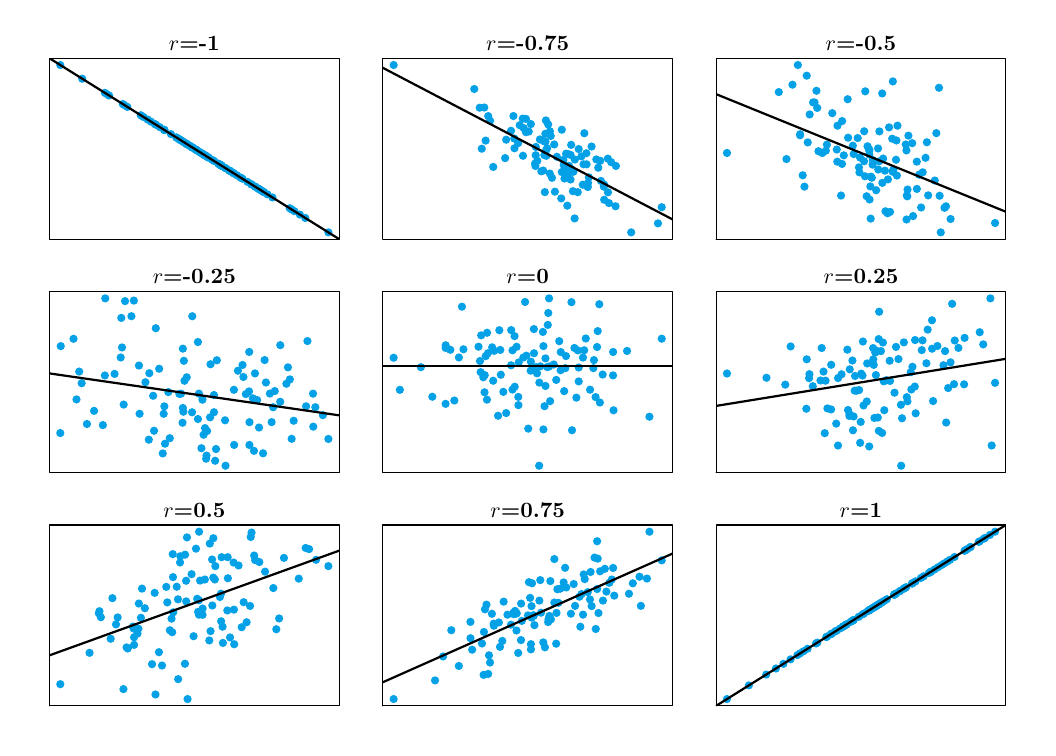
\begin{tikzpicture}[x=1pt,y=1pt]
\definecolor{fillColor}{RGB}{255,255,255}
\path[use as bounding box,fill=fillColor,fill opacity=0.00] (0,0) rectangle (361.35,252.94);
\begin{scope}
\path[clip] (  7.92,176.55) rectangle (112.53,241.86);
\definecolor{fillColor}{RGB}{5,161,230}

\path[fill=fillColor] ( 34.83,225.06) circle (  1.49);

\path[fill=fillColor] ( 57.37,210.99) circle (  1.49);

\path[fill=fillColor] ( 47.72,217.01) circle (  1.49);

\path[fill=fillColor] ( 60.53,209.02) circle (  1.49);

\path[fill=fillColor] ( 68.84,203.83) circle (  1.49);

\path[fill=fillColor] ( 69.51,203.41) circle (  1.49);

\path[fill=fillColor] ( 59.64,209.57) circle (  1.49);

\path[fill=fillColor] ( 56.31,211.65) circle (  1.49);

\path[fill=fillColor] ( 46.35,217.87) circle (  1.49);

\path[fill=fillColor] ( 49.43,215.94) circle (  1.49);

\path[fill=fillColor] ( 55.63,212.07) circle (  1.49);

\path[fill=fillColor] ( 63.20,207.35) circle (  1.49);

\path[fill=fillColor] ( 70.11,203.03) circle (  1.49);

\path[fill=fillColor] ( 63.40,207.22) circle (  1.49);

\path[fill=fillColor] ( 57.58,210.86) circle (  1.49);

\path[fill=fillColor] ( 28.57,228.97) circle (  1.49);

\path[fill=fillColor] ( 95.36,187.27) circle (  1.49);

\path[fill=fillColor] ( 71.32,202.28) circle (  1.49);

\path[fill=fillColor] ( 54.58,212.73) circle (  1.49);

\path[fill=fillColor] ( 58.68,210.17) circle (  1.49);

\path[fill=fillColor] ( 64.07,206.80) circle (  1.49);

\path[fill=fillColor] ( 96.35,186.65) circle (  1.49);

\path[fill=fillColor] ( 45.95,218.12) circle (  1.49);

\path[fill=fillColor] ( 29.44,228.42) circle (  1.49);

\path[fill=fillColor] ( 69.90,203.16) circle (  1.49);

\path[fill=fillColor] ( 63.45,207.19) circle (  1.49);

\path[fill=fillColor] ( 57.14,211.13) circle (  1.49);

\path[fill=fillColor] ( 65.11,206.15) circle (  1.49);

\path[fill=fillColor] ( 53.67,213.30) circle (  1.49);

\path[fill=fillColor] ( 57.52,210.89) circle (  1.49);

\path[fill=fillColor] ( 65.40,205.97) circle (  1.49);

\path[fill=fillColor] ( 61.18,208.61) circle (  1.49);

\path[fill=fillColor] ( 58.49,210.29) circle (  1.49);

\path[fill=fillColor] ( 44.58,218.97) circle (  1.49);

\path[fill=fillColor] ( 27.90,229.39) circle (  1.49);

\path[fill=fillColor] ( 85.37,193.50) circle (  1.49);

\path[fill=fillColor] ( 83.86,194.45) circle (  1.49);

\path[fill=fillColor] ( 59.50,209.65) circle (  1.49);

\path[fill=fillColor] ( 55.34,212.25) circle (  1.49);

\path[fill=fillColor] ( 88.44,191.59) circle (  1.49);

\path[fill=fillColor] ( 75.54,199.64) circle (  1.49);

\path[fill=fillColor] ( 72.90,201.29) circle (  1.49);

\path[fill=fillColor] ( 62.28,207.92) circle (  1.49);

\path[fill=fillColor] ( 62.15,208.00) circle (  1.49);

\path[fill=fillColor] ( 40.86,221.29) circle (  1.49);

\path[fill=fillColor] ( 77.09,198.68) circle (  1.49);

\path[fill=fillColor] ( 57.64,210.81) circle (  1.49);

\path[fill=fillColor] ( 73.60,200.86) circle (  1.49);

\path[fill=fillColor] ( 64.40,206.60) circle (  1.49);

\path[fill=fillColor] ( 19.71,234.49) circle (  1.49);

\path[fill=fillColor] ( 62.68,207.67) circle (  1.49);

\path[fill=fillColor] ( 80.77,196.38) circle (  1.49);

\path[fill=fillColor] ( 60.71,208.90) circle (  1.49);

\path[fill=fillColor] ( 74.29,200.42) circle (  1.49);

\path[fill=fillColor] ( 76.85,198.82) circle (  1.49);

\path[fill=fillColor] ( 41.84,220.68) circle (  1.49);

\path[fill=fillColor] ( 56.42,211.58) circle (  1.49);

\path[fill=fillColor] ( 94.68,187.69) circle (  1.49);

\path[fill=fillColor] ( 74.46,200.32) circle (  1.49);

\path[fill=fillColor] ( 49.25,216.06) circle (  1.49);

\path[fill=fillColor] ( 54.81,212.59) circle (  1.49);

\path[fill=fillColor] ( 63.92,206.89) circle (  1.49);

\path[fill=fillColor] ( 83.44,194.71) circle (  1.49);

\path[fill=fillColor] ( 64.34,206.63) circle (  1.49);

\path[fill=fillColor] ( 53.90,213.15) circle (  1.49);

\path[fill=fillColor] ( 69.22,203.59) circle (  1.49);

\path[fill=fillColor] ( 80.89,196.31) circle (  1.49);

\path[fill=fillColor] ( 57.29,211.03) circle (  1.49);

\path[fill=fillColor] ( 83.19,194.87) circle (  1.49);

\path[fill=fillColor] ( 77.65,198.33) circle (  1.49);

\path[fill=fillColor] ( 73.07,201.18) circle (  1.49);

\path[fill=fillColor] ( 86.67,192.70) circle (  1.49);

\path[fill=fillColor] ( 66.77,205.11) circle (  1.49);

\path[fill=fillColor] ( 51.75,214.49) circle (  1.49);

\path[fill=fillColor] ( 61.09,208.66) circle (  1.49);

\path[fill=fillColor] ( 36.02,224.31) circle (  1.49);

\path[fill=fillColor] ( 98.35,185.40) circle (  1.49);

\path[fill=fillColor] ( 59.45,209.69) circle (  1.49);

\path[fill=fillColor] ( 11.79,239.44) circle (  1.49);

\path[fill=fillColor] ( 34.38,225.34) circle (  1.49);

\path[fill=fillColor] ( 79.44,197.21) circle (  1.49);

\path[fill=fillColor] ( 65.23,206.08) circle (  1.49);

\path[fill=fillColor] ( 69.73,203.27) circle (  1.49);

\path[fill=fillColor] ( 43.38,219.72) circle (  1.49);

\path[fill=fillColor] (108.66,178.97) circle (  1.49);

\path[fill=fillColor] ( 49.38,215.98) circle (  1.49);

\path[fill=fillColor] ( 70.16,203.00) circle (  1.49);

\path[fill=fillColor] ( 85.12,193.66) circle (  1.49);

\path[fill=fillColor] (100.31,184.18) circle (  1.49);

\path[fill=fillColor] ( 59.36,209.74) circle (  1.49);

\path[fill=fillColor] ( 84.57,194.00) circle (  1.49);

\path[fill=fillColor] ( 71.71,202.03) circle (  1.49);

\path[fill=fillColor] ( 82.23,195.47) circle (  1.49);

\path[fill=fillColor] ( 82.12,195.53) circle (  1.49);

\path[fill=fillColor] ( 70.13,203.02) circle (  1.49);

\path[fill=fillColor] ( 73.04,201.20) circle (  1.49);

\path[fill=fillColor] ( 55.07,212.42) circle (  1.49);

\path[fill=fillColor] ( 83.92,194.41) circle (  1.49);

\path[fill=fillColor] ( 69.38,203.49) circle (  1.49);

\path[fill=fillColor] ( 67.35,204.76) circle (  1.49);
\end{scope}
\begin{scope}
\path[clip] (  0.00,168.63) rectangle (120.45,252.94);
\definecolor{drawColor}{RGB}{0,0,0}

\node[text=drawColor,anchor=base,inner sep=0pt, outer sep=0pt, scale=  0.79] at ( 60.22,244.63) {\bfseries $r$=-1};

\node[text=drawColor,anchor=base,inner sep=0pt, outer sep=0pt, scale=  0.66] at ( 60.22,146.45) {$X$};
\end{scope}
\begin{scope}
\path[clip] (  7.92,176.55) rectangle (112.53,241.86);
\definecolor{drawColor}{RGB}{0,0,0}

\path[draw=drawColor,line width= 0.8pt,line join=round,line cap=round] (  7.92,241.86) -- (112.53,176.55);
\end{scope}
\begin{scope}
\path[clip] (  0.00,  0.00) rectangle (361.35,252.94);
\definecolor{drawColor}{RGB}{0,0,0}

\path[draw=drawColor,line width= 0.4pt,line join=round,line cap=round] (  7.92,176.55) --
	(112.53,176.55) --
	(112.53,241.86) --
	(  7.92,241.86) --
	(  7.92,176.55);
\end{scope}
\begin{scope}
\path[clip] (128.37,176.55) rectangle (232.98,241.86);
\definecolor{fillColor}{RGB}{5,161,230}

\path[fill=fillColor] (196.17,198.07) circle (  1.49);

\path[fill=fillColor] (208.32,190.76) circle (  1.49);

\path[fill=fillColor] (183.57,206.85) circle (  1.49);

\path[fill=fillColor] (174.65,215.66) circle (  1.49);

\path[fill=fillColor] (218.08,178.97) circle (  1.49);

\path[fill=fillColor] (167.10,219.28) circle (  1.49);

\path[fill=fillColor] (199.11,209.08) circle (  1.49);

\path[fill=fillColor] (201.96,203.56) circle (  1.49);

\path[fill=fillColor] (186.70,206.91) circle (  1.49);

\path[fill=fillColor] (201.89,207.56) circle (  1.49);

\path[fill=fillColor] (181.84,218.10) circle (  1.49);

\path[fill=fillColor] (205.48,205.33) circle (  1.49);

\path[fill=fillColor] (206.88,204.83) circle (  1.49);

\path[fill=fillColor] (172.91,212.46) circle (  1.49);

\path[fill=fillColor] (178.88,220.07) circle (  1.49);

\path[fill=fillColor] (198.77,193.50) circle (  1.49);

\path[fill=fillColor] (192.80,191.23) circle (  1.49);

\path[fill=fillColor] (187.06,214.58) circle (  1.49);

\path[fill=fillColor] (172.53,205.80) circle (  1.49);

\path[fill=fillColor] (187.33,208.67) circle (  1.49);

\path[fill=fillColor] (227.76,182.22) circle (  1.49);

\path[fill=fillColor] (161.38,230.78) circle (  1.49);

\path[fill=fillColor] (188.69,200.21) circle (  1.49);

\path[fill=fillColor] (208.18,195.48) circle (  1.49);

\path[fill=fillColor] (183.64,209.83) circle (  1.49);

\path[fill=fillColor] (165.48,212.13) circle (  1.49);

\path[fill=fillColor] (189.46,198.68) circle (  1.49);

\path[fill=fillColor] (132.24,239.44) circle (  1.49);

\path[fill=fillColor] (178.97,206.65) circle (  1.49);

\path[fill=fillColor] (175.84,212.87) circle (  1.49);

\path[fill=fillColor] (191.24,206.28) circle (  1.49);

\path[fill=fillColor] (196.18,206.97) circle (  1.49);

\path[fill=fillColor] (179.24,216.66) circle (  1.49);

\path[fill=fillColor] (183.32,203.80) circle (  1.49);

\path[fill=fillColor] (187.11,211.75) circle (  1.49);

\path[fill=fillColor] (181.07,215.41) circle (  1.49);

\path[fill=fillColor] (190.51,193.68) circle (  1.49);

\path[fill=fillColor] (186.87,193.51) circle (  1.49);

\path[fill=fillColor] (210.04,189.55) circle (  1.49);

\path[fill=fillColor] (208.29,196.24) circle (  1.49);

\path[fill=fillColor] (212.56,202.97) circle (  1.49);

\path[fill=fillColor] (195.16,199.85) circle (  1.49);

\path[fill=fillColor] (202.28,195.68) circle (  1.49);

\path[fill=fillColor] (193.58,205.14) circle (  1.49);

\path[fill=fillColor] (185.59,201.05) circle (  1.49);

\path[fill=fillColor] (186.43,211.94) circle (  1.49);

\path[fill=fillColor] (194.99,188.62) circle (  1.49);

\path[fill=fillColor] (175.90,209.36) circle (  1.49);

\path[fill=fillColor] (180.04,215.18) circle (  1.49);

\path[fill=fillColor] (210.84,204.34) circle (  1.49);

\path[fill=fillColor] (187.26,219.42) circle (  1.49);

\path[fill=fillColor] (206.18,202.33) circle (  1.49);

\path[fill=fillColor] (193.70,203.27) circle (  1.49);

\path[fill=fillColor] (202.49,196.82) circle (  1.49);

\path[fill=fillColor] (193.98,198.43) circle (  1.49);

\path[fill=fillColor] (168.23,202.62) circle (  1.49);

\path[fill=fillColor] (188.71,215.51) circle (  1.49);

\path[fill=fillColor] (196.39,210.60) circle (  1.49);

\path[fill=fillColor] (190.27,210.74) circle (  1.49);

\path[fill=fillColor] (200.86,203.57) circle (  1.49);

\path[fill=fillColor] (183.48,202.96) circle (  1.49);

\path[fill=fillColor] (195.27,207.26) circle (  1.49);

\path[fill=fillColor] (163.34,224.02) circle (  1.49);

\path[fill=fillColor] (207.15,197.57) circle (  1.49);

\path[fill=fillColor] (193.01,200.76) circle (  1.49);

\path[fill=fillColor] (196.41,201.81) circle (  1.49);

\path[fill=fillColor] (185.09,212.55) circle (  1.49);

\path[fill=fillColor] (202.77,198.85) circle (  1.49);

\path[fill=fillColor] (175.52,221.01) circle (  1.49);

\path[fill=fillColor] (195.62,203.01) circle (  1.49);

\path[fill=fillColor] (177.80,217.70) circle (  1.49);

\path[fill=fillColor] (202.39,195.35) circle (  1.49);

\path[fill=fillColor] (187.42,206.64) circle (  1.49);

\path[fill=fillColor] (197.02,193.85) circle (  1.49);

\path[fill=fillColor] (180.05,219.97) circle (  1.49);

\path[fill=fillColor] (166.41,220.98) circle (  1.49);

\path[fill=fillColor] (200.08,206.43) circle (  1.49);

\path[fill=fillColor] (197.71,205.28) circle (  1.49);

\path[fill=fillColor] (212.43,188.41) circle (  1.49);

\path[fill=fillColor] (165.00,224.09) circle (  1.49);

\path[fill=fillColor] (187.71,209.37) circle (  1.49);

\path[fill=fillColor] (193.00,216.06) circle (  1.49);

\path[fill=fillColor] (209.65,205.62) circle (  1.49);

\path[fill=fillColor] (186.29,201.29) circle (  1.49);

\path[fill=fillColor] (197.64,184.01) circle (  1.49);

\path[fill=fillColor] (200.58,196.19) circle (  1.49);

\path[fill=fillColor] (189.00,213.81) circle (  1.49);

\path[fill=fillColor] (193.84,201.35) circle (  1.49);

\path[fill=fillColor] (195.45,200.56) circle (  1.49);

\path[fill=fillColor] (209.69,193.45) circle (  1.49);

\path[fill=fillColor] (188.08,217.99) circle (  1.49);

\path[fill=fillColor] (194.53,207.39) circle (  1.49);

\path[fill=fillColor] (229.11,188.07) circle (  1.49);

\path[fill=fillColor] (164.08,209.20) circle (  1.49);

\path[fill=fillColor] (184.16,204.83) circle (  1.49);

\path[fill=fillColor] (201.14,214.79) circle (  1.49);

\path[fill=fillColor] (203.76,209.99) circle (  1.49);

\path[fill=fillColor] (197.20,200.87) circle (  1.49);

\path[fill=fillColor] (177.25,211.24) circle (  1.49);

\path[fill=fillColor] (196.25,200.79) circle (  1.49);
\end{scope}
\begin{scope}
\path[clip] (120.45,168.63) rectangle (240.90,252.94);
\definecolor{drawColor}{RGB}{0,0,0}

\node[text=drawColor,anchor=base,inner sep=0pt, outer sep=0pt, scale=  0.79] at (180.68,244.63) {\bfseries $r$=-0.75};

\node[text=drawColor,anchor=base,inner sep=0pt, outer sep=0pt, scale=  0.66] at (180.68,146.45) {$X$};

\node[text=drawColor,rotate= 90.00,anchor=base,inner sep=0pt, outer sep=0pt, scale=  0.66] at (103.03,209.20) {$Y$};
\end{scope}
\begin{scope}
\path[clip] (128.37,176.55) rectangle (232.98,241.86);
\definecolor{drawColor}{RGB}{0,0,0}

\path[draw=drawColor,line width= 0.8pt,line join=round,line cap=round] (128.37,238.41) -- (232.98,183.67);
\end{scope}
\begin{scope}
\path[clip] (  0.00,  0.00) rectangle (361.35,252.94);
\definecolor{drawColor}{RGB}{0,0,0}

\path[draw=drawColor,line width= 0.4pt,line join=round,line cap=round] (128.37,176.55) --
	(232.98,176.55) --
	(232.98,241.86) --
	(128.37,241.86) --
	(128.37,176.55);
\end{scope}
\begin{scope}
\path[clip] (248.82,176.55) rectangle (353.43,241.86);
\definecolor{fillColor}{RGB}{5,161,230}

\path[fill=fillColor] (299.93,213.05) circle (  1.49);

\path[fill=fillColor] (324.45,205.91) circle (  1.49);

\path[fill=fillColor] (298.48,207.26) circle (  1.49);

\path[fill=fillColor] (284.35,225.91) circle (  1.49);

\path[fill=fillColor] (324.92,211.53) circle (  1.49);

\path[fill=fillColor] (252.69,207.66) circle (  1.49);

\path[fill=fillColor] (305.39,205.08) circle (  1.49);

\path[fill=fillColor] (303.15,192.02) circle (  1.49);

\path[fill=fillColor] (312.83,201.68) circle (  1.49);

\path[fill=fillColor] (329.94,178.97) circle (  1.49);

\path[fill=fillColor] (309.12,205.64) circle (  1.49);

\path[fill=fillColor] (292.55,204.51) circle (  1.49);

\path[fill=fillColor] (294.27,203.70) circle (  1.49);

\path[fill=fillColor] (288.80,210.69) circle (  1.49);

\path[fill=fillColor] (296.46,213.17) circle (  1.49);

\path[fill=fillColor] (304.07,209.01) circle (  1.49);

\path[fill=fillColor] (313.78,205.21) circle (  1.49);

\path[fill=fillColor] (281.87,211.48) circle (  1.49);

\path[fill=fillColor] (300.79,205.99) circle (  1.49);

\path[fill=fillColor] (311.62,186.36) circle (  1.49);

\path[fill=fillColor] (302.57,199.24) circle (  1.49);

\path[fill=fillColor] (313.91,212.18) circle (  1.49);

\path[fill=fillColor] (309.97,186.59) circle (  1.49);

\path[fill=fillColor] (285.30,223.94) circle (  1.49);

\path[fill=fillColor] (285.03,230.13) circle (  1.49);

\path[fill=fillColor] (302.66,229.93) circle (  1.49);

\path[fill=fillColor] (305.03,198.72) circle (  1.49);

\path[fill=fillColor] (302.27,215.50) circle (  1.49);

\path[fill=fillColor] (333.49,183.80) circle (  1.49);

\path[fill=fillColor] (304.23,190.85) circle (  1.49);

\path[fill=fillColor] (314.30,217.53) circle (  1.49);

\path[fill=fillColor] (298.17,210.28) circle (  1.49);

\path[fill=fillColor] (312.51,200.90) circle (  1.49);

\path[fill=fillColor] (309.76,201.27) circle (  1.49);

\path[fill=fillColor] (294.90,206.80) circle (  1.49);

\path[fill=fillColor] (318.25,213.92) circle (  1.49);

\path[fill=fillColor] (308.78,229.17) circle (  1.49);

\path[fill=fillColor] (310.87,198.12) circle (  1.49);

\path[fill=fillColor] (319.93,184.86) circle (  1.49);

\path[fill=fillColor] (304.50,195.58) circle (  1.49);

\path[fill=fillColor] (331.82,188.39) circle (  1.49);

\path[fill=fillColor] (329.53,192.20) circle (  1.49);

\path[fill=fillColor] (290.75,222.04) circle (  1.49);

\path[fill=fillColor] (307.34,201.69) circle (  1.49);

\path[fill=fillColor] (307.76,215.46) circle (  1.49);

\path[fill=fillColor] (305.31,203.44) circle (  1.49);

\path[fill=fillColor] (317.58,183.62) circle (  1.49);

\path[fill=fillColor] (323.40,200.67) circle (  1.49);

\path[fill=fillColor] (329.30,231.22) circle (  1.49);

\path[fill=fillColor] (300.38,202.46) circle (  1.49);

\path[fill=fillColor] (303.48,210.07) circle (  1.49);

\path[fill=fillColor] (276.36,232.34) circle (  1.49);

\path[fill=fillColor] (285.75,208.29) circle (  1.49);

\path[fill=fillColor] (306.60,194.20) circle (  1.49);

\path[fill=fillColor] (317.55,208.59) circle (  1.49);

\path[fill=fillColor] (319.62,211.19) circle (  1.49);

\path[fill=fillColor] (304.11,208.50) circle (  1.49);

\path[fill=fillColor] (317.29,210.73) circle (  1.49);

\path[fill=fillColor] (317.69,192.36) circle (  1.49);

\path[fill=fillColor] (328.34,214.82) circle (  1.49);

\path[fill=fillColor] (302.22,204.67) circle (  1.49);

\path[fill=fillColor] (279.12,214.43) circle (  1.49);

\path[fill=fillColor] (321.29,204.53) circle (  1.49);

\path[fill=fillColor] (283.79,225.92) circle (  1.49);

\path[fill=fillColor] (304.70,199.10) circle (  1.49);

\path[fill=fillColor] (325.39,192.34) circle (  1.49);

\path[fill=fillColor] (288.42,208.50) circle (  1.49);

\path[fill=fillColor] (281.51,235.59) circle (  1.49);

\path[fill=fillColor] (307.28,209.29) circle (  1.49);

\path[fill=fillColor] (322.84,187.96) circle (  1.49);

\path[fill=fillColor] (274.19,205.45) circle (  1.49);

\path[fill=fillColor] (312.63,233.51) circle (  1.49);

\path[fill=fillColor] (279.10,214.07) circle (  1.49);

\path[fill=fillColor] (310.70,185.88) circle (  1.49);

\path[fill=fillColor] (293.91,192.28) circle (  1.49);

\path[fill=fillColor] (317.86,192.00) circle (  1.49);

\path[fill=fillColor] (317.94,194.44) circle (  1.49);

\path[fill=fillColor] (321.31,194.67) circle (  1.49);

\path[fill=fillColor] (308.83,196.85) circle (  1.49);

\path[fill=fillColor] (296.31,227.08) circle (  1.49);

\path[fill=fillColor] (294.31,219.19) circle (  1.49);

\path[fill=fillColor] (300.56,200.65) circle (  1.49);

\path[fill=fillColor] (287.14,207.63) circle (  1.49);

\path[fill=fillColor] (280.68,195.50) circle (  1.49);

\path[fill=fillColor] (292.62,217.51) circle (  1.49);

\path[fill=fillColor] (278.30,239.44) circle (  1.49);

\path[fill=fillColor] (322.14,199.82) circle (  1.49);

\path[fill=fillColor] (282.57,221.59) circle (  1.49);

\path[fill=fillColor] (304.12,207.11) circle (  1.49);

\path[fill=fillColor] (331.29,187.84) circle (  1.49);

\path[fill=fillColor] (304.62,183.94) circle (  1.49);

\path[fill=fillColor] (314.09,199.50) circle (  1.49);

\path[fill=fillColor] (311.26,216.91) circle (  1.49);

\path[fill=fillColor] (349.56,182.35) circle (  1.49);

\path[fill=fillColor] (292.37,208.91) circle (  1.49);

\path[fill=fillColor] (307.71,204.66) circle (  1.49);

\path[fill=fillColor] (280.05,199.60) circle (  1.49);

\path[fill=fillColor] (271.41,229.66) circle (  1.49);

\path[fill=fillColor] (327.78,197.70) circle (  1.49);

\path[fill=fillColor] (312.39,212.82) circle (  1.49);
\end{scope}
\begin{scope}
\path[clip] (240.90,168.63) rectangle (361.35,252.94);
\definecolor{drawColor}{RGB}{0,0,0}

\node[text=drawColor,anchor=base,inner sep=0pt, outer sep=0pt, scale=  0.79] at (301.12,244.63) {\bfseries $r$=-0.5};

\node[text=drawColor,anchor=base,inner sep=0pt, outer sep=0pt, scale=  0.66] at (301.12,146.45) {$X$};

\node[text=drawColor,rotate= 90.00,anchor=base,inner sep=0pt, outer sep=0pt, scale=  0.66] at (223.48,209.20) {$Y$};
\end{scope}
\begin{scope}
\path[clip] (248.82,176.55) rectangle (353.43,241.86);
\definecolor{drawColor}{RGB}{0,0,0}

\path[draw=drawColor,line width= 0.8pt,line join=round,line cap=round] (248.82,228.90) -- (353.43,186.43);
\end{scope}
\begin{scope}
\path[clip] (  0.00,  0.00) rectangle (361.35,252.94);
\definecolor{drawColor}{RGB}{0,0,0}

\path[draw=drawColor,line width= 0.4pt,line join=round,line cap=round] (248.82,176.55) --
	(353.43,176.55) --
	(353.43,241.86) --
	(248.82,241.86) --
	(248.82,176.55);
\end{scope}
\begin{scope}
\path[clip] (  7.92, 92.23) rectangle (112.53,157.54);
\definecolor{fillColor}{RGB}{5,161,230}

\path[fill=fillColor] ( 88.70,115.78) circle (  1.49);

\path[fill=fillColor] ( 28.04,155.12) circle (  1.49);

\path[fill=fillColor] ( 71.33,111.06) circle (  1.49);

\path[fill=fillColor] ( 56.07,136.96) circle (  1.49);

\path[fill=fillColor] ( 64.83,107.20) circle (  1.49);

\path[fill=fillColor] ( 16.57,140.51) circle (  1.49);

\path[fill=fillColor] ( 65.91,112.12) circle (  1.49);

\path[fill=fillColor] ( 43.77,104.06) circle (  1.49);

\path[fill=fillColor] ( 74.61,102.16) circle (  1.49);

\path[fill=fillColor] ( 83.60,108.45) circle (  1.49);

\path[fill=fillColor] (103.12,120.69) circle (  1.49);

\path[fill=fillColor] ( 49.39,116.10) circle (  1.49);

\path[fill=fillColor] ( 77.63,131.06) circle (  1.49);

\path[fill=fillColor] ( 63.57,105.84) circle (  1.49);

\path[fill=fillColor] ( 55.96,110.18) circle (  1.49);

\path[fill=fillColor] ( 71.50, 94.65) circle (  1.49);

\path[fill=fillColor] (101.09,139.70) circle (  1.49);

\path[fill=fillColor] ( 75.97,128.98) circle (  1.49);

\path[fill=fillColor] ( 94.05,130.20) circle (  1.49);

\path[fill=fillColor] ( 19.50,124.46) circle (  1.49);

\path[fill=fillColor] ( 68.05,100.67) circle (  1.49);

\path[fill=fillColor] ( 61.88,120.70) circle (  1.49);

\path[fill=fillColor] ( 43.96,128.07) circle (  1.49);

\path[fill=fillColor] ( 62.78,100.97) circle (  1.49);

\path[fill=fillColor] ( 21.42,109.73) circle (  1.49);

\path[fill=fillColor] ( 47.52,129.69) circle (  1.49);

\path[fill=fillColor] (103.20,108.77) circle (  1.49);

\path[fill=fillColor] ( 96.12,110.90) circle (  1.49);

\path[fill=fillColor] ( 49.63,102.61) circle (  1.49);

\path[fill=fillColor] ( 50.82,121.26) circle (  1.49);

\path[fill=fillColor] (106.67,112.92) circle (  1.49);

\path[fill=fillColor] ( 31.41,127.83) circle (  1.49);

\path[fill=fillColor] ( 67.32,113.97) circle (  1.49);

\path[fill=fillColor] ( 51.35,104.59) circle (  1.49);

\path[fill=fillColor] (100.60,116.12) circle (  1.49);

\path[fill=fillColor] ( 94.74,125.85) circle (  1.49);

\path[fill=fillColor] ( 57.48,126.61) circle (  1.49);

\path[fill=fillColor] ( 64.48, 97.18) circle (  1.49);

\path[fill=fillColor] ( 66.06,131.31) circle (  1.49);

\path[fill=fillColor] ( 80.12,102.15) circle (  1.49);

\path[fill=fillColor] ( 56.26,114.17) circle (  1.49);

\path[fill=fillColor] ( 81.76,100.03) circle (  1.49);

\path[fill=fillColor] ( 86.09,124.72) circle (  1.49);

\path[fill=fillColor] ( 82.13,128.01) circle (  1.49);

\path[fill=fillColor] ( 81.38,119.00) circle (  1.49);

\path[fill=fillColor] ( 91.26,117.75) circle (  1.49);

\path[fill=fillColor] ( 33.83,148.07) circle (  1.49);

\path[fill=fillColor] ( 37.49,148.67) circle (  1.49);

\path[fill=fillColor] ( 35.18,154.13) circle (  1.49);

\path[fill=fillColor] ( 88.15,110.40) circle (  1.49);

\path[fill=fillColor] ( 89.27,121.62) circle (  1.49);

\path[fill=fillColor] ( 34.09,137.39) circle (  1.49);

\path[fill=fillColor] ( 48.81, 99.09) circle (  1.49);

\path[fill=fillColor] ( 59.48,148.66) circle (  1.49);

\path[fill=fillColor] ( 80.06,135.77) circle (  1.49);

\path[fill=fillColor] ( 85.05, 99.14) circle (  1.49);

\path[fill=fillColor] ( 45.34,119.93) circle (  1.49);

\path[fill=fillColor] ( 18.62,128.67) circle (  1.49);

\path[fill=fillColor] ( 79.99,121.51) circle (  1.49);

\path[fill=fillColor] ( 40.21,130.85) circle (  1.49);

\path[fill=fillColor] (108.66,104.32) circle (  1.49);

\path[fill=fillColor] ( 45.67,107.28) circle (  1.49);

\path[fill=fillColor] ( 64.08,108.25) circle (  1.49);

\path[fill=fillColor] ( 11.79,106.46) circle (  1.49);

\path[fill=fillColor] ( 55.42,120.68) circle (  1.49);

\path[fill=fillColor] ( 87.52,120.72) circle (  1.49);

\path[fill=fillColor] ( 61.53,111.53) circle (  1.49);

\path[fill=fillColor] ( 46.30,144.34) circle (  1.49);

\path[fill=fillColor] ( 27.89,127.26) circle (  1.49);

\path[fill=fillColor] ( 23.99,114.47) circle (  1.49);

\path[fill=fillColor] ( 56.07,115.52) circle (  1.49);

\path[fill=fillColor] ( 56.44,132.56) circle (  1.49);

\path[fill=fillColor] ( 63.15,118.51) circle (  1.49);

\path[fill=fillColor] ( 61.52,139.34) circle (  1.49);

\path[fill=fillColor] ( 17.64,118.62) circle (  1.49);

\path[fill=fillColor] ( 38.36,154.32) circle (  1.49);

\path[fill=fillColor] ( 54.81,120.60) circle (  1.49);

\path[fill=fillColor] ( 42.55,124.82) circle (  1.49);

\path[fill=fillColor] ( 27.17,109.33) circle (  1.49);

\path[fill=fillColor] ( 77.96,126.73) circle (  1.49);

\path[fill=fillColor] ( 59.40,113.96) circle (  1.49);

\path[fill=fillColor] ( 74.53,122.08) circle (  1.49);

\path[fill=fillColor] ( 78.83,120.53) circle (  1.49);

\path[fill=fillColor] ( 56.66,125.35) circle (  1.49);

\path[fill=fillColor] ( 82.92,118.37) circle (  1.49);

\path[fill=fillColor] ( 95.38,104.37) circle (  1.49);

\path[fill=fillColor] ( 85.62,132.83) circle (  1.49);

\path[fill=fillColor] ( 64.63, 98.32) circle (  1.49);

\path[fill=fillColor] ( 49.15,113.40) circle (  1.49);

\path[fill=fillColor] ( 67.32,120.19) circle (  1.49);

\path[fill=fillColor] ( 33.61,133.76) circle (  1.49);

\path[fill=fillColor] ( 11.95,137.86) circle (  1.49);

\path[fill=fillColor] ( 34.69,116.75) circle (  1.49);

\path[fill=fillColor] ( 80.16,110.38) circle (  1.49);

\path[fill=fillColor] ( 93.49,124.27) circle (  1.49);

\path[fill=fillColor] ( 67.74, 96.45) circle (  1.49);

\path[fill=fillColor] ( 68.35,132.75) circle (  1.49);

\path[fill=fillColor] ( 40.44,113.43) circle (  1.49);

\path[fill=fillColor] (103.94,115.79) circle (  1.49);

\path[fill=fillColor] ( 91.28,138.21) circle (  1.49);
\end{scope}
\begin{scope}
\path[clip] (  0.00, 84.31) rectangle (120.45,168.63);
\definecolor{drawColor}{RGB}{0,0,0}

\node[text=drawColor,anchor=base,inner sep=0pt, outer sep=0pt, scale=  0.79] at ( 60.22,160.32) {\bfseries $r$=-0.25};

\node[text=drawColor,anchor=base,inner sep=0pt, outer sep=0pt, scale=  0.66] at ( 60.22, 62.14) {$X$};
\end{scope}
\begin{scope}
\path[clip] (  7.92, 92.23) rectangle (112.53,157.54);
\definecolor{drawColor}{RGB}{0,0,0}

\path[draw=drawColor,line width= 0.8pt,line join=round,line cap=round] (  7.92,128.00) -- (112.53,112.86);
\end{scope}
\begin{scope}
\path[clip] (  0.00,  0.00) rectangle (361.35,252.94);
\definecolor{drawColor}{RGB}{0,0,0}

\path[draw=drawColor,line width= 0.4pt,line join=round,line cap=round] (  7.92, 92.23) --
	(112.53, 92.23) --
	(112.53,157.54) --
	(  7.92,157.54) --
	(  7.92, 92.23);
\end{scope}
\begin{scope}
\path[clip] (128.37, 92.23) rectangle (232.98,157.54);
\definecolor{fillColor}{RGB}{5,161,230}

\path[fill=fillColor] (180.21,134.42) circle (  1.49);

\path[fill=fillColor] (196.70,107.47) circle (  1.49);

\path[fill=fillColor] (174.72,143.66) circle (  1.49);

\path[fill=fillColor] (186.37,137.87) circle (  1.49);

\path[fill=fillColor] (187.10,133.43) circle (  1.49);

\path[fill=fillColor] (199.11,125.12) circle (  1.49);

\path[fill=fillColor] (175.94,141.47) circle (  1.49);

\path[fill=fillColor] (164.63,126.62) circle (  1.49);

\path[fill=fillColor] (168.22,125.35) circle (  1.49);

\path[fill=fillColor] (132.24,133.67) circle (  1.49);

\path[fill=fillColor] (179.73,153.82) circle (  1.49);

\path[fill=fillColor] (163.87,141.76) circle (  1.49);

\path[fill=fillColor] (211.54,135.75) circle (  1.49);

\path[fill=fillColor] (151.02,117.01) circle (  1.49);

\path[fill=fillColor] (186.36,107.77) circle (  1.49);

\path[fill=fillColor] (181.75,128.99) circle (  1.49);

\path[fill=fillColor] (179.10,133.74) circle (  1.49);

\path[fill=fillColor] (162.91,137.65) circle (  1.49);

\path[fill=fillColor] (198.27,119.25) circle (  1.49);

\path[fill=fillColor] (157.46,136.73) circle (  1.49);

\path[fill=fillColor] (188.12,149.84) circle (  1.49);

\path[fill=fillColor] (204.41,129.91) circle (  1.49);

\path[fill=fillColor] (176.66,137.63) circle (  1.49);

\path[fill=fillColor] (197.58,137.20) circle (  1.49);

\path[fill=fillColor] (196.50,153.75) circle (  1.49);

\path[fill=fillColor] (186.77,116.16) circle (  1.49);

\path[fill=fillColor] (151.03,137.21) circle (  1.49);

\path[fill=fillColor] (192.08,139.66) circle (  1.49);

\path[fill=fillColor] (205.98,143.30) circle (  1.49);

\path[fill=fillColor] (175.99,123.19) circle (  1.49);

\path[fill=fillColor] (165.51,134.25) circle (  1.49);

\path[fill=fillColor] (216.58,136.12) circle (  1.49);

\path[fill=fillColor] (156.92,152.12) circle (  1.49);

\path[fill=fillColor] (166.31,135.31) circle (  1.49);

\path[fill=fillColor] (151.04,138.17) circle (  1.49);

\path[fill=fillColor] (201.10,136.37) circle (  1.49);

\path[fill=fillColor] (224.67,112.36) circle (  1.49);

\path[fill=fillColor] (170.97,127.53) circle (  1.49);

\path[fill=fillColor] (175.20,136.35) circle (  1.49);

\path[fill=fillColor] (154.18,118.21) circle (  1.49);

\path[fill=fillColor] (198.79,136.32) circle (  1.49);

\path[fill=fillColor] (205.22,119.45) circle (  1.49);

\path[fill=fillColor] (229.11,140.55) circle (  1.49);

\path[fill=fillColor] (184.82, 94.65) circle (  1.49);

\path[fill=fillColor] (188.78,117.98) circle (  1.49);

\path[fill=fillColor] (169.98,112.71) circle (  1.49);

\path[fill=fillColor] (174.68,130.94) circle (  1.49);

\path[fill=fillColor] (177.28,119.52) circle (  1.49);

\path[fill=fillColor] (134.49,122.07) circle (  1.49);

\path[fill=fillColor] (168.55,136.16) circle (  1.49);

\path[fill=fillColor] (211.70,114.68) circle (  1.49);

\path[fill=fillColor] (184.89,124.68) circle (  1.49);

\path[fill=fillColor] (170.43,143.61) circle (  1.49);

\path[fill=fillColor] (188.45,130.51) circle (  1.49);

\path[fill=fillColor] (206.77,117.48) circle (  1.49);

\path[fill=fillColor] (163.68,128.46) circle (  1.49);

\path[fill=fillColor] (205.75,137.54) circle (  1.49);

\path[fill=fillColor] (182.91,144.03) circle (  1.49);

\path[fill=fillColor] (200.64,133.73) circle (  1.49);

\path[fill=fillColor] (165.08,121.19) circle (  1.49);

\path[fill=fillColor] (187.75,130.29) circle (  1.49);

\path[fill=fillColor] (186.17,142.99) circle (  1.49);

\path[fill=fillColor] (187.94,145.53) circle (  1.49);

\path[fill=fillColor] (165.96,118.53) circle (  1.49);

\path[fill=fillColor] (181.85,132.23) circle (  1.49);

\path[fill=fillColor] (185.24,130.57) circle (  1.49);

\path[fill=fillColor] (175.18,122.17) circle (  1.49);

\path[fill=fillColor] (182.96,135.29) circle (  1.49);

\path[fill=fillColor] (142.09,130.26) circle (  1.49);

\path[fill=fillColor] (165.16,127.39) circle (  1.49);

\path[fill=fillColor] (177.44,131.99) circle (  1.49);

\path[fill=fillColor] (155.82,133.77) circle (  1.49);

\path[fill=fillColor] (171.88,121.34) circle (  1.49);

\path[fill=fillColor] (146.22,119.58) circle (  1.49);

\path[fill=fillColor] (211.52,127.29) circle (  1.49);

\path[fill=fillColor] (194.29,129.91) circle (  1.49);

\path[fill=fillColor] (152.73,136.53) circle (  1.49);

\path[fill=fillColor] (177.33,116.55) circle (  1.49);

\path[fill=fillColor] (192.57,129.15) circle (  1.49);

\path[fill=fillColor] (167.84,137.43) circle (  1.49);

\path[fill=fillColor] (172.91,113.68) circle (  1.49);

\path[fill=fillColor] (201.67,140.62) circle (  1.49);

\path[fill=fillColor] (206.55,153.00) circle (  1.49);

\path[fill=fillColor] (187.11,123.47) circle (  1.49);

\path[fill=fillColor] (199.12,130.14) circle (  1.49);

\path[fill=fillColor] (188.41,155.12) circle (  1.49);

\path[fill=fillColor] (194.53,134.27) circle (  1.49);

\path[fill=fillColor] (190.09,131.23) circle (  1.49);

\path[fill=fillColor] (183.68,130.27) circle (  1.49);

\path[fill=fillColor] (193.87,121.60) circle (  1.49);

\path[fill=fillColor] (192.63,135.72) circle (  1.49);

\path[fill=fillColor] (163.44,132.47) circle (  1.49);

\path[fill=fillColor] (166.00,142.69) circle (  1.49);

\path[fill=fillColor] (191.00,125.66) circle (  1.49);

\path[fill=fillColor] (170.77,136.49) circle (  1.49);

\path[fill=fillColor] (204.62,132.82) circle (  1.49);

\path[fill=fillColor] (207.77,127.60) circle (  1.49);

\path[fill=fillColor] (180.88,108.05) circle (  1.49);

\path[fill=fillColor] (184.06,128.02) circle (  1.49);

\path[fill=fillColor] (203.21,122.12) circle (  1.49);
\end{scope}
\begin{scope}
\path[clip] (120.45, 84.31) rectangle (240.90,168.63);
\definecolor{drawColor}{RGB}{0,0,0}

\node[text=drawColor,anchor=base,inner sep=0pt, outer sep=0pt, scale=  0.79] at (180.68,160.32) {\bfseries $r$=0};

\node[text=drawColor,anchor=base,inner sep=0pt, outer sep=0pt, scale=  0.66] at (180.68, 62.14) {$X$};

\node[text=drawColor,rotate= 90.00,anchor=base,inner sep=0pt, outer sep=0pt, scale=  0.66] at (103.03,124.89) {$Y$};
\end{scope}
\begin{scope}
\path[clip] (128.37, 92.23) rectangle (232.98,157.54);
\definecolor{drawColor}{RGB}{0,0,0}

\path[draw=drawColor,line width= 0.8pt,line join=round,line cap=round] (128.37,130.66) -- (232.98,130.66);
\end{scope}
\begin{scope}
\path[clip] (  0.00,  0.00) rectangle (361.35,252.94);
\definecolor{drawColor}{RGB}{0,0,0}

\path[draw=drawColor,line width= 0.4pt,line join=round,line cap=round] (128.37, 92.23) --
	(232.98, 92.23) --
	(232.98,157.54) --
	(128.37,157.54) --
	(128.37, 92.23);
\end{scope}
\begin{scope}
\path[clip] (248.82, 92.23) rectangle (353.43,157.54);
\definecolor{fillColor}{RGB}{5,161,230}

\path[fill=fillColor] (305.71,131.09) circle (  1.49);

\path[fill=fillColor] (327.17,118.02) circle (  1.49);

\path[fill=fillColor] (344.02,142.88) circle (  1.49);

\path[fill=fillColor] (281.37,115.24) circle (  1.49);

\path[fill=fillColor] (296.19,136.58) circle (  1.49);

\path[fill=fillColor] (332.61,122.72) circle (  1.49);

\path[fill=fillColor] (345.29,138.49) circle (  1.49);

\path[fill=fillColor] (334.99,139.89) circle (  1.49);

\path[fill=fillColor] (296.92,112.64) circle (  1.49);

\path[fill=fillColor] (331.89,110.26) circle (  1.49);

\path[fill=fillColor] (316.60,139.22) circle (  1.49);

\path[fill=fillColor] (303.35,131.60) circle (  1.49);

\path[fill=fillColor] (319.31,122.20) circle (  1.49);

\path[fill=fillColor] (347.87,155.12) circle (  1.49);

\path[fill=fillColor] (334.74,124.12) circle (  1.49);

\path[fill=fillColor] (298.97,127.09) circle (  1.49);

\path[fill=fillColor] (320.66,140.06) circle (  1.49);

\path[fill=fillColor] (294.09,127.69) circle (  1.49);

\path[fill=fillColor] (296.97,113.28) circle (  1.49);

\path[fill=fillColor] (288.02,106.41) circle (  1.49);

\path[fill=fillColor] (325.21,143.83) circle (  1.49);

\path[fill=fillColor] (323.35,139.95) circle (  1.49);

\path[fill=fillColor] (315.94,111.80) circle (  1.49);

\path[fill=fillColor] (304.09,101.62) circle (  1.49);

\path[fill=fillColor] (303.21,117.87) circle (  1.49);

\path[fill=fillColor] (292.80,101.95) circle (  1.49);

\path[fill=fillColor] (331.50,136.07) circle (  1.49);

\path[fill=fillColor] (323.07,136.42) circle (  1.49);

\path[fill=fillColor] (333.47,132.00) circle (  1.49);

\path[fill=fillColor] (349.56,124.60) circle (  1.49);

\path[fill=fillColor] (286.47,125.45) circle (  1.49);

\path[fill=fillColor] (336.32,137.23) circle (  1.49);

\path[fill=fillColor] (296.42,114.78) circle (  1.49);

\path[fill=fillColor] (309.53,114.70) circle (  1.49);

\path[fill=fillColor] (288.99,115.36) circle (  1.49);

\path[fill=fillColor] (324.76,131.68) circle (  1.49);

\path[fill=fillColor] (311.61,125.29) circle (  1.49);

\path[fill=fillColor] (281.51,133.10) circle (  1.49);

\path[fill=fillColor] (292.84,126.33) circle (  1.49);

\path[fill=fillColor] (338.38,124.06) circle (  1.49);

\path[fill=fillColor] (320.56,123.26) circle (  1.49);

\path[fill=fillColor] (307.00,136.08) circle (  1.49);

\path[fill=fillColor] (319.71,130.40) circle (  1.49);

\path[fill=fillColor] (252.69,127.97) circle (  1.49);

\path[fill=fillColor] (326.78,147.21) circle (  1.49);

\path[fill=fillColor] (288.31,125.38) circle (  1.49);

\path[fill=fillColor] (286.92,137.18) circle (  1.49);

\path[fill=fillColor] (266.96,126.43) circle (  1.49);

\path[fill=fillColor] (298.22,107.46) circle (  1.49);

\path[fill=fillColor] (302.04,116.43) circle (  1.49);

\path[fill=fillColor] (305.56,133.08) circle (  1.49);

\path[fill=fillColor] (309.04,139.16) circle (  1.49);

\path[fill=fillColor] (282.49,127.73) circle (  1.49);

\path[fill=fillColor] (320.87,113.58) circle (  1.49);

\path[fill=fillColor] (306.27,135.56) circle (  1.49);

\path[fill=fillColor] (317.90,117.93) circle (  1.49);

\path[fill=fillColor] (310.28,125.55) circle (  1.49);

\path[fill=fillColor] (313.77,137.58) circle (  1.49);

\path[fill=fillColor] (299.51,121.77) circle (  1.49);

\path[fill=fillColor] (300.81,102.92) circle (  1.49);

\path[fill=fillColor] (301.21,127.92) circle (  1.49);

\path[fill=fillColor] (307.68,150.29) circle (  1.49);

\path[fill=fillColor] (330.92,130.96) circle (  1.49);

\path[fill=fillColor] (298.01,132.66) circle (  1.49);

\path[fill=fillColor] (283.69,123.38) circle (  1.49);

\path[fill=fillColor] (313.23,121.04) circle (  1.49);

\path[fill=fillColor] (308.75,106.48) circle (  1.49);

\path[fill=fillColor] (290.35,131.12) circle (  1.49);

\path[fill=fillColor] (338.55,140.84) circle (  1.49);

\path[fill=fillColor] (319.10,128.44) circle (  1.49);

\path[fill=fillColor] (311.48,132.58) circle (  1.49);

\path[fill=fillColor] (307.56,107.24) circle (  1.49);

\path[fill=fillColor] (348.34,101.96) circle (  1.49);

\path[fill=fillColor] (315.54,116.67) circle (  1.49);

\path[fill=fillColor] (292.17,109.87) circle (  1.49);

\path[fill=fillColor] (301.01,110.48) circle (  1.49);

\path[fill=fillColor] (307.50,140.41) circle (  1.49);

\path[fill=fillColor] (326.81,136.93) circle (  1.49);

\path[fill=fillColor] (273.76,123.95) circle (  1.49);

\path[fill=fillColor] (290.31,114.99) circle (  1.49);

\path[fill=fillColor] (308.33,136.07) circle (  1.49);

\path[fill=fillColor] (328.73,137.91) circle (  1.49);

\path[fill=fillColor] (307.19,112.07) circle (  1.49);

\path[fill=fillColor] (334.05,153.15) circle (  1.49);

\path[fill=fillColor] (300.43,121.98) circle (  1.49);

\path[fill=fillColor] (315.63, 94.65) circle (  1.49);

\path[fill=fillColor] (305.96,111.91) circle (  1.49);

\path[fill=fillColor] (317.67,119.42) circle (  1.49);

\path[fill=fillColor] (287.57,128.66) circle (  1.49);

\path[fill=fillColor] (298.84,121.78) circle (  1.49);

\path[fill=fillColor] (301.66,127.23) circle (  1.49);

\path[fill=fillColor] (309.34,125.15) circle (  1.49);

\path[fill=fillColor] (282.36,126.29) circle (  1.49);

\path[fill=fillColor] (301.81,139.53) circle (  1.49);

\path[fill=fillColor] (297.05,129.48) circle (  1.49);

\path[fill=fillColor] (314.66,133.18) circle (  1.49);

\path[fill=fillColor] (305.50,137.16) circle (  1.49);

\path[fill=fillColor] (275.69,137.75) circle (  1.49);

\path[fill=fillColor] (306.50,127.41) circle (  1.49);

\path[fill=fillColor] (298.45,112.45) circle (  1.49);
\end{scope}
\begin{scope}
\path[clip] (240.90, 84.31) rectangle (361.35,168.63);
\definecolor{drawColor}{RGB}{0,0,0}

\node[text=drawColor,anchor=base,inner sep=0pt, outer sep=0pt, scale=  0.79] at (301.12,160.32) {\bfseries $r$=0.25};

\node[text=drawColor,anchor=base,inner sep=0pt, outer sep=0pt, scale=  0.66] at (301.12, 62.14) {$X$};

\node[text=drawColor,rotate= 90.00,anchor=base,inner sep=0pt, outer sep=0pt, scale=  0.66] at (223.48,124.89) {$Y$};
\end{scope}
\begin{scope}
\path[clip] (248.82, 92.23) rectangle (353.43,157.54);
\definecolor{drawColor}{RGB}{0,0,0}

\path[draw=drawColor,line width= 0.8pt,line join=round,line cap=round] (248.82,116.27) -- (353.43,133.27);
\end{scope}
\begin{scope}
\path[clip] (  0.00,  0.00) rectangle (361.35,252.94);
\definecolor{drawColor}{RGB}{0,0,0}

\path[draw=drawColor,line width= 0.4pt,line join=round,line cap=round] (248.82, 92.23) --
	(353.43, 92.23) --
	(353.43,157.54) --
	(248.82,157.54) --
	(248.82, 92.23);
\end{scope}
\begin{scope}
\path[clip] (  7.92,  7.92) rectangle (112.53, 73.23);
\definecolor{fillColor}{RGB}{5,161,230}

\path[fill=fillColor] (104.21, 60.64) circle (  1.49);

\path[fill=fillColor] ( 69.47, 47.21) circle (  1.49);

\path[fill=fillColor] ( 47.43, 27.27) circle (  1.49);

\path[fill=fillColor] ( 97.95, 53.85) circle (  1.49);

\path[fill=fillColor] ( 61.58, 41.84) circle (  1.49);

\path[fill=fillColor] ( 82.20, 60.55) circle (  1.49);

\path[fill=fillColor] ( 69.90, 38.44) circle (  1.49);

\path[fill=fillColor] ( 60.82, 64.68) circle (  1.49);

\path[fill=fillColor] ( 72.34, 53.98) circle (  1.49);

\path[fill=fillColor] ( 41.31, 50.24) circle (  1.49);

\path[fill=fillColor] ( 63.21, 43.04) circle (  1.49);

\path[fill=fillColor] ( 81.84, 62.20) circle (  1.49);

\path[fill=fillColor] ( 61.94, 70.81) circle (  1.49);

\path[fill=fillColor] ( 63.20, 40.76) circle (  1.49);

\path[fill=fillColor] ( 38.44, 32.66) circle (  1.49);

\path[fill=fillColor] ( 38.04, 36.52) circle (  1.49);

\path[fill=fillColor] (101.69, 64.52) circle (  1.49);

\path[fill=fillColor] ( 59.95, 33.04) circle (  1.49);

\path[fill=fillColor] ( 52.42, 62.70) circle (  1.49);

\path[fill=fillColor] ( 66.08, 34.88) circle (  1.49);

\path[fill=fillColor] ( 34.60, 13.93) circle (  1.49);

\path[fill=fillColor] ( 72.27, 61.60) circle (  1.49);

\path[fill=fillColor] ( 22.36, 27.04) circle (  1.49);

\path[fill=fillColor] ( 88.76, 50.44) circle (  1.49);

\path[fill=fillColor] ( 50.45, 45.27) circle (  1.49);

\path[fill=fillColor] ( 90.86, 39.46) circle (  1.49);

\path[fill=fillColor] ( 35.75, 29.01) circle (  1.49);

\path[fill=fillColor] ( 62.29, 53.14) circle (  1.49);

\path[fill=fillColor] ( 53.85, 50.92) circle (  1.49);

\path[fill=fillColor] ( 67.63, 53.54) circle (  1.49);

\path[fill=fillColor] ( 74.52, 42.65) circle (  1.49);

\path[fill=fillColor] ( 25.94, 42.08) circle (  1.49);

\path[fill=fillColor] ( 65.63, 31.52) circle (  1.49);

\path[fill=fillColor] ( 66.63, 60.76) circle (  1.49);

\path[fill=fillColor] ( 57.56, 68.75) circle (  1.49);

\path[fill=fillColor] ( 70.08, 61.60) circle (  1.49);

\path[fill=fillColor] ( 74.63, 30.14) circle (  1.49);

\path[fill=fillColor] ( 80.90, 70.50) circle (  1.49);

\path[fill=fillColor] ( 51.38, 35.18) circle (  1.49);

\path[fill=fillColor] ( 64.01, 53.52) circle (  1.49);

\path[fill=fillColor] ( 52.59, 41.68) circle (  1.49);

\path[fill=fillColor] ( 30.62, 46.79) circle (  1.49);

\path[fill=fillColor] ( 52.22, 34.49) circle (  1.49);

\path[fill=fillColor] ( 57.78, 10.34) circle (  1.49);

\path[fill=fillColor] ( 69.85, 48.39) circle (  1.49);

\path[fill=fillColor] ( 74.41, 59.66) circle (  1.49);

\path[fill=fillColor] ( 76.21, 58.60) circle (  1.49);

\path[fill=fillColor] ( 55.06, 59.69) circle (  1.49);

\path[fill=fillColor] ( 77.33, 36.30) circle (  1.49);

\path[fill=fillColor] ( 66.72, 44.14) circle (  1.49);

\path[fill=fillColor] ( 85.78, 56.38) circle (  1.49);

\path[fill=fillColor] ( 46.18, 11.99) circle (  1.49);

\path[fill=fillColor] ( 57.26, 53.08) circle (  1.49);

\path[fill=fillColor] ( 40.01, 35.76) circle (  1.49);

\path[fill=fillColor] ( 89.85, 35.55) circle (  1.49);

\path[fill=fillColor] ( 83.72, 59.84) circle (  1.49);

\path[fill=fillColor] ( 61.87, 46.06) circle (  1.49);

\path[fill=fillColor] ( 51.99, 39.39) circle (  1.49);

\path[fill=fillColor] ( 45.89, 48.72) circle (  1.49);

\path[fill=fillColor] ( 38.29, 35.80) circle (  1.49);

\path[fill=fillColor] ( 32.51, 39.84) circle (  1.49);

\path[fill=fillColor] ( 57.28, 45.63) circle (  1.49);

\path[fill=fillColor] ( 31.92, 37.31) circle (  1.49);

\path[fill=fillColor] ( 61.26, 46.56) circle (  1.49);

\path[fill=fillColor] ( 70.44, 36.48) circle (  1.49);

\path[fill=fillColor] ( 67.10, 68.47) circle (  1.49);

\path[fill=fillColor] ( 61.88, 40.82) circle (  1.49);

\path[fill=fillColor] ( 70.55, 30.62) circle (  1.49);

\path[fill=fillColor] (108.66, 58.37) circle (  1.49);

\path[fill=fillColor] ( 54.38, 17.54) circle (  1.49);

\path[fill=fillColor] ( 59.23, 55.46) circle (  1.49);

\path[fill=fillColor] ( 11.79, 15.70) circle (  1.49);

\path[fill=fillColor] ( 40.17, 44.85) circle (  1.49);

\path[fill=fillColor] ( 40.91, 39.70) circle (  1.49);

\path[fill=fillColor] ( 54.31, 46.38) circle (  1.49);

\path[fill=fillColor] ( 80.60, 68.90) circle (  1.49);

\path[fill=fillColor] ( 67.82, 58.36) circle (  1.49);

\path[fill=fillColor] ( 80.35, 43.98) circle (  1.49);

\path[fill=fillColor] ( 92.60, 61.34) circle (  1.49);

\path[fill=fillColor] ( 38.45, 29.91) circle (  1.49);

\path[fill=fillColor] ( 50.08, 50.87) circle (  1.49);

\path[fill=fillColor] ( 52.51, 54.40) circle (  1.49);

\path[fill=fillColor] ( 36.16, 28.61) circle (  1.49);

\path[fill=fillColor] ( 48.54, 22.45) circle (  1.49);

\path[fill=fillColor] ( 56.83, 23.09) circle (  1.49);

\path[fill=fillColor] ( 55.17, 61.94) circle (  1.49);

\path[fill=fillColor] ( 42.34, 43.16) circle (  1.49);

\path[fill=fillColor] ( 65.81, 66.52) circle (  1.49);

\path[fill=fillColor] ( 25.72, 41.30) circle (  1.49);

\path[fill=fillColor] ( 26.45, 39.91) circle (  1.49);

\path[fill=fillColor] (100.44, 64.93) circle (  1.49);

\path[fill=fillColor] ( 44.94, 22.94) circle (  1.49);

\path[fill=fillColor] ( 78.04, 45.34) circle (  1.49);

\path[fill=fillColor] ( 29.99, 32.12) circle (  1.49);

\path[fill=fillColor] ( 72.14, 42.35) circle (  1.49);

\path[fill=fillColor] ( 56.88, 62.51) circle (  1.49);

\path[fill=fillColor] ( 39.70, 34.00) circle (  1.49);

\path[fill=fillColor] ( 67.08, 54.22) circle (  1.49);

\path[fill=fillColor] ( 79.11, 38.09) circle (  1.49);

\path[fill=fillColor] ( 73.13, 32.60) circle (  1.49);
\end{scope}
\begin{scope}
\path[clip] (  0.00,  0.00) rectangle (120.45, 84.31);
\definecolor{drawColor}{RGB}{0,0,0}

\node[text=drawColor,anchor=base,inner sep=0pt, outer sep=0pt, scale=  0.79] at ( 60.22, 76.00) {\bfseries $r$=0.5};
\end{scope}
\begin{scope}
\path[clip] (  7.92,  7.92) rectangle (112.53, 73.23);
\definecolor{drawColor}{RGB}{0,0,0}

\path[draw=drawColor,line width= 0.8pt,line join=round,line cap=round] (  7.92, 26.14) -- (112.53, 63.95);
\end{scope}
\begin{scope}
\path[clip] (  0.00,  0.00) rectangle (361.35,252.94);
\definecolor{drawColor}{RGB}{0,0,0}

\path[draw=drawColor,line width= 0.4pt,line join=round,line cap=round] (  7.92,  7.92) --
	(112.53,  7.92) --
	(112.53, 73.23) --
	(  7.92, 73.23) --
	(  7.92,  7.92);
\end{scope}
\begin{scope}
\path[clip] (128.37,  7.92) rectangle (232.98, 73.23);
\definecolor{fillColor}{RGB}{5,161,230}

\path[fill=fillColor] (203.78, 43.93) circle (  1.49);

\path[fill=fillColor] (200.93, 55.37) circle (  1.49);

\path[fill=fillColor] (175.52, 41.54) circle (  1.49);

\path[fill=fillColor] (221.58, 44.01) circle (  1.49);

\path[fill=fillColor] (194.20, 57.76) circle (  1.49);

\path[fill=fillColor] (175.60, 41.03) circle (  1.49);

\path[fill=fillColor] (159.99, 38.22) circle (  1.49);

\path[fill=fillColor] (204.84, 61.45) circle (  1.49);

\path[fill=fillColor] (167.07, 23.54) circle (  1.49);

\path[fill=fillColor] (176.14, 42.18) circle (  1.49);

\path[fill=fillColor] (171.99, 45.53) circle (  1.49);

\path[fill=fillColor] (150.11, 25.73) circle (  1.49);

\path[fill=fillColor] (160.61, 28.18) circle (  1.49);

\path[fill=fillColor] (153.07, 35.21) circle (  1.49);

\path[fill=fillColor] (183.12, 37.04) circle (  1.49);

\path[fill=fillColor] (218.67, 52.17) circle (  1.49);

\path[fill=fillColor] (211.55, 57.71) circle (  1.49);

\path[fill=fillColor] (186.91, 29.03) circle (  1.49);

\path[fill=fillColor] (189.07, 39.14) circle (  1.49);

\path[fill=fillColor] (188.87, 52.97) circle (  1.49);

\path[fill=fillColor] (191.41, 50.03) circle (  1.49);

\path[fill=fillColor] (170.27, 38.03) circle (  1.49);

\path[fill=fillColor] (202.38, 48.97) circle (  1.49);

\path[fill=fillColor] (190.30, 45.21) circle (  1.49);

\path[fill=fillColor] (178.26, 31.64) circle (  1.49);

\path[fill=fillColor] (193.67, 52.48) circle (  1.49);

\path[fill=fillColor] (164.87, 34.58) circle (  1.49);

\path[fill=fillColor] (217.27, 48.39) circle (  1.49);

\path[fill=fillColor] (208.55, 57.41) circle (  1.49);

\path[fill=fillColor] (203.19, 46.33) circle (  1.49);

\path[fill=fillColor] (190.32, 60.92) circle (  1.49);

\path[fill=fillColor] (197.80, 43.99) circle (  1.49);

\path[fill=fillColor] (155.80, 22.29) circle (  1.49);

\path[fill=fillColor] (207.87, 45.91) circle (  1.49);

\path[fill=fillColor] (178.30, 44.83) circle (  1.49);

\path[fill=fillColor] (182.78, 40.62) circle (  1.49);

\path[fill=fillColor] (180.77, 40.57) circle (  1.49);

\path[fill=fillColor] (188.06, 38.15) circle (  1.49);

\path[fill=fillColor] (188.20, 39.23) circle (  1.49);

\path[fill=fillColor] (176.03, 41.07) circle (  1.49);

\path[fill=fillColor] (200.67, 40.84) circle (  1.49);

\path[fill=fillColor] (191.09, 41.47) circle (  1.49);

\path[fill=fillColor] (182.85, 40.43) circle (  1.49);

\path[fill=fillColor] (165.23, 42.76) circle (  1.49);

\path[fill=fillColor] (209.12, 49.16) circle (  1.49);

\path[fill=fillColor] (178.56, 38.58) circle (  1.49);

\path[fill=fillColor] (167.76, 41.15) circle (  1.49);

\path[fill=fillColor] (176.62, 35.10) circle (  1.49);

\path[fill=fillColor] (206.25, 41.42) circle (  1.49);

\path[fill=fillColor] (182.07, 43.91) circle (  1.49);

\path[fill=fillColor] (205.27, 35.66) circle (  1.49);

\path[fill=fillColor] (211.96, 47.71) circle (  1.49);

\path[fill=fillColor] (132.24, 10.34) circle (  1.49);

\path[fill=fillColor] (181.84, 30.17) circle (  1.49);

\path[fill=fillColor] (181.85, 28.29) circle (  1.49);

\path[fill=fillColor] (186.31, 30.81) circle (  1.49);

\path[fill=fillColor] (181.13, 52.57) circle (  1.49);

\path[fill=fillColor] (229.11, 60.45) circle (  1.49);

\path[fill=fillColor] (160.01, 32.32) circle (  1.49);

\path[fill=fillColor] (199.71, 36.48) circle (  1.49);

\path[fill=fillColor] (173.38, 40.82) circle (  1.49);

\path[fill=fillColor] (197.30, 51.90) circle (  1.49);

\path[fill=fillColor] (221.09, 54.54) circle (  1.49);

\path[fill=fillColor] (164.75, 19.08) circle (  1.49);

\path[fill=fillColor] (201.29, 53.67) circle (  1.49);

\path[fill=fillColor] (205.77, 67.36) circle (  1.49);

\path[fill=fillColor] (224.69, 70.81) circle (  1.49);

\path[fill=fillColor] (223.77, 53.88) circle (  1.49);

\path[fill=fillColor] (192.44, 50.22) circle (  1.49);

\path[fill=fillColor] (211.07, 53.53) circle (  1.49);

\path[fill=fillColor] (182.25, 52.18) circle (  1.49);

\path[fill=fillColor] (185.50, 41.54) circle (  1.49);

\path[fill=fillColor] (166.69, 26.14) circle (  1.49);

\path[fill=fillColor] (166.39, 19.41) circle (  1.49);

\path[fill=fillColor] (147.21, 17.08) circle (  1.49);

\path[fill=fillColor] (171.51, 31.33) circle (  1.49);

\path[fill=fillColor] (188.51, 40.37) circle (  1.49);

\path[fill=fillColor] (203.41, 56.26) circle (  1.49);

\path[fill=fillColor] (177.25, 26.99) circle (  1.49);

\path[fill=fillColor] (168.37, 37.57) circle (  1.49);

\path[fill=fillColor] (170.68, 29.20) circle (  1.49);

\path[fill=fillColor] (176.73, 41.29) circle (  1.49);

\path[fill=fillColor] (210.18, 52.34) circle (  1.49);

\path[fill=fillColor] (205.78, 50.10) circle (  1.49);

\path[fill=fillColor] (194.61, 50.66) circle (  1.49);

\path[fill=fillColor] (205.99, 61.08) circle (  1.49);

\path[fill=fillColor] (200.12, 48.26) circle (  1.49);

\path[fill=fillColor] (182.11, 39.75) circle (  1.49);

\path[fill=fillColor] (181.55, 46.90) circle (  1.49);

\path[fill=fillColor] (184.90, 45.91) circle (  1.49);

\path[fill=fillColor] (196.29, 41.18) circle (  1.49);

\path[fill=fillColor] (164.17, 30.41) circle (  1.49);

\path[fill=fillColor] (168.45, 36.83) circle (  1.49);

\path[fill=fillColor] (190.98, 30.35) circle (  1.49);

\path[fill=fillColor] (199.40, 47.32) circle (  1.49);

\path[fill=fillColor] (165.79, 44.45) circle (  1.49);

\path[fill=fillColor] (174.65, 37.22) circle (  1.49);

\path[fill=fillColor] (191.78, 45.10) circle (  1.49);

\path[fill=fillColor] (206.85, 56.50) circle (  1.49);

\path[fill=fillColor] (185.23, 53.31) circle (  1.49);
\end{scope}
\begin{scope}
\path[clip] (120.45,  0.00) rectangle (240.90, 84.31);
\definecolor{drawColor}{RGB}{0,0,0}

\node[text=drawColor,anchor=base,inner sep=0pt, outer sep=0pt, scale=  0.79] at (180.68, 76.00) {\bfseries $r$=0.75};

\node[text=drawColor,rotate= 90.00,anchor=base,inner sep=0pt, outer sep=0pt, scale=  0.66] at (103.03, 40.57) {$Y$};
\end{scope}
\begin{scope}
\path[clip] (128.37,  7.92) rectangle (232.98, 73.23);
\definecolor{drawColor}{RGB}{0,0,0}

\path[draw=drawColor,line width= 0.8pt,line join=round,line cap=round] (128.37, 16.43) -- (232.98, 62.89);
\end{scope}
\begin{scope}
\path[clip] (  0.00,  0.00) rectangle (361.35,252.94);
\definecolor{drawColor}{RGB}{0,0,0}

\path[draw=drawColor,line width= 0.4pt,line join=round,line cap=round] (128.37,  7.92) --
	(232.98,  7.92) --
	(232.98, 73.23) --
	(128.37, 73.23) --
	(128.37,  7.92);
\end{scope}
\begin{scope}
\path[clip] (248.82,  7.92) rectangle (353.43, 73.23);
\definecolor{fillColor}{RGB}{5,161,230}

\path[fill=fillColor] (294.74, 36.59) circle (  1.49);

\path[fill=fillColor] (347.72, 69.66) circle (  1.49);

\path[fill=fillColor] (315.26, 49.40) circle (  1.49);

\path[fill=fillColor] (297.84, 38.52) circle (  1.49);

\path[fill=fillColor] (339.07, 64.26) circle (  1.49);

\path[fill=fillColor] (333.29, 60.65) circle (  1.49);

\path[fill=fillColor] (345.95, 68.56) circle (  1.49);

\path[fill=fillColor] (304.27, 42.54) circle (  1.49);

\path[fill=fillColor] (293.60, 35.87) circle (  1.49);

\path[fill=fillColor] (300.29, 40.05) circle (  1.49);

\path[fill=fillColor] (332.29, 60.03) circle (  1.49);

\path[fill=fillColor] (325.68, 55.90) circle (  1.49);

\path[fill=fillColor] (298.20, 38.75) circle (  1.49);

\path[fill=fillColor] (305.14, 43.08) circle (  1.49);

\path[fill=fillColor] (295.82, 37.26) circle (  1.49);

\path[fill=fillColor] (307.12, 44.32) circle (  1.49);

\path[fill=fillColor] (326.36, 56.33) circle (  1.49);

\path[fill=fillColor] (290.30, 33.81) circle (  1.49);

\path[fill=fillColor] (290.65, 34.04) circle (  1.49);

\path[fill=fillColor] (304.57, 42.73) circle (  1.49);

\path[fill=fillColor] (339.53, 64.55) circle (  1.49);

\path[fill=fillColor] (302.25, 41.28) circle (  1.49);

\path[fill=fillColor] (252.69, 10.34) circle (  1.49);

\path[fill=fillColor] (343.67, 67.13) circle (  1.49);

\path[fill=fillColor] (315.11, 49.31) circle (  1.49);

\path[fill=fillColor] (308.42, 45.13) circle (  1.49);

\path[fill=fillColor] (297.36, 38.23) circle (  1.49);

\path[fill=fillColor] (316.43, 50.13) circle (  1.49);

\path[fill=fillColor] (298.51, 38.94) circle (  1.49);

\path[fill=fillColor] (306.75, 44.08) circle (  1.49);

\path[fill=fillColor] (313.55, 48.33) circle (  1.49);

\path[fill=fillColor] (305.96, 43.59) circle (  1.49);

\path[fill=fillColor] (308.59, 45.24) circle (  1.49);

\path[fill=fillColor] (323.77, 54.71) circle (  1.49);

\path[fill=fillColor] (279.18, 26.88) circle (  1.49);

\path[fill=fillColor] (317.41, 50.74) circle (  1.49);

\path[fill=fillColor] (303.95, 42.34) circle (  1.49);

\path[fill=fillColor] (326.43, 56.37) circle (  1.49);

\path[fill=fillColor] (303.56, 42.09) circle (  1.49);

\path[fill=fillColor] (334.92, 61.67) circle (  1.49);

\path[fill=fillColor] (319.52, 52.06) circle (  1.49);

\path[fill=fillColor] (309.53, 45.82) circle (  1.49);

\path[fill=fillColor] (305.41, 43.25) circle (  1.49);

\path[fill=fillColor] (307.51, 44.56) circle (  1.49);

\path[fill=fillColor] (284.87, 30.43) circle (  1.49);

\path[fill=fillColor] (301.63, 40.89) circle (  1.49);

\path[fill=fillColor] (313.83, 48.51) circle (  1.49);

\path[fill=fillColor] (344.00, 67.34) circle (  1.49);

\path[fill=fillColor] (288.56, 32.73) circle (  1.49);

\path[fill=fillColor] (307.74, 44.71) circle (  1.49);

\path[fill=fillColor] (329.05, 58.01) circle (  1.49);

\path[fill=fillColor] (313.07, 48.03) circle (  1.49);

\path[fill=fillColor] (273.07, 23.06) circle (  1.49);

\path[fill=fillColor] (280.37, 27.62) circle (  1.49);

\path[fill=fillColor] (307.60, 44.61) circle (  1.49);

\path[fill=fillColor] (304.13, 42.45) circle (  1.49);

\path[fill=fillColor] (317.20, 50.61) circle (  1.49);

\path[fill=fillColor] (295.69, 37.18) circle (  1.49);

\path[fill=fillColor] (320.82, 52.87) circle (  1.49);

\path[fill=fillColor] (288.93, 32.96) circle (  1.49);

\path[fill=fillColor] (340.69, 65.27) circle (  1.49);

\path[fill=fillColor] (305.64, 43.39) circle (  1.49);

\path[fill=fillColor] (306.77, 44.10) circle (  1.49);

\path[fill=fillColor] (295.82, 37.26) circle (  1.49);

\path[fill=fillColor] (313.10, 48.05) circle (  1.49);

\path[fill=fillColor] (313.17, 48.10) circle (  1.49);

\path[fill=fillColor] (322.79, 54.10) circle (  1.49);

\path[fill=fillColor] (308.76, 45.34) circle (  1.49);

\path[fill=fillColor] (330.30, 58.79) circle (  1.49);

\path[fill=fillColor] (326.30, 56.29) circle (  1.49);

\path[fill=fillColor] (304.41, 42.62) circle (  1.49);

\path[fill=fillColor] (338.66, 64.01) circle (  1.49);

\path[fill=fillColor] (270.38, 21.38) circle (  1.49);

\path[fill=fillColor] (281.81, 28.51) circle (  1.49);

\path[fill=fillColor] (278.15, 26.23) circle (  1.49);

\path[fill=fillColor] (260.60, 15.28) circle (  1.49);

\path[fill=fillColor] (295.76, 37.22) circle (  1.49);

\path[fill=fillColor] (294.75, 36.59) circle (  1.49);

\path[fill=fillColor] (291.80, 34.75) circle (  1.49);

\path[fill=fillColor] (327.78, 57.21) circle (  1.49);

\path[fill=fillColor] (345.45, 68.25) circle (  1.49);

\path[fill=fillColor] (306.36, 43.84) circle (  1.49);

\path[fill=fillColor] (340.64, 65.25) circle (  1.49);

\path[fill=fillColor] (298.23, 38.77) circle (  1.49);

\path[fill=fillColor] (349.56, 70.81) circle (  1.49);

\path[fill=fillColor] (331.22, 59.36) circle (  1.49);

\path[fill=fillColor] (319.64, 52.13) circle (  1.49);

\path[fill=fillColor] (310.48, 46.42) circle (  1.49);

\path[fill=fillColor] (319.87, 52.28) circle (  1.49);

\path[fill=fillColor] (338.55, 63.94) circle (  1.49);

\path[fill=fillColor] (316.81, 50.37) circle (  1.49);

\path[fill=fillColor] (292.30, 35.06) circle (  1.49);

\path[fill=fillColor] (306.47, 43.91) circle (  1.49);

\path[fill=fillColor] (285.34, 30.72) circle (  1.49);

\path[fill=fillColor] (290.26, 33.79) circle (  1.49);

\path[fill=fillColor] (307.49, 44.55) circle (  1.49);

\path[fill=fillColor] (266.85, 19.17) circle (  1.49);

\path[fill=fillColor] (294.57, 36.48) circle (  1.49);

\path[fill=fillColor] (275.66, 24.68) circle (  1.49);

\path[fill=fillColor] (313.22, 48.13) circle (  1.49);
\end{scope}
\begin{scope}
\path[clip] (240.90,  0.00) rectangle (361.35, 84.31);
\definecolor{drawColor}{RGB}{0,0,0}

\node[text=drawColor,anchor=base,inner sep=0pt, outer sep=0pt, scale=  0.79] at (301.12, 76.00) {\bfseries $r$=1};

\node[text=drawColor,rotate= 90.00,anchor=base,inner sep=0pt, outer sep=0pt, scale=  0.66] at (223.48, 40.57) {$Y$};
\end{scope}
\begin{scope}
\path[clip] (248.82,  7.92) rectangle (353.43, 73.23);
\definecolor{drawColor}{RGB}{0,0,0}

\path[draw=drawColor,line width= 0.8pt,line join=round,line cap=round] (248.82,  7.92) -- (353.43, 73.23);
\end{scope}
\begin{scope}
\path[clip] (  0.00,  0.00) rectangle (361.35,252.94);
\definecolor{drawColor}{RGB}{0,0,0}

\path[draw=drawColor,line width= 0.4pt,line join=round,line cap=round] (248.82,  7.92) --
	(353.43,  7.92) --
	(353.43, 73.23) --
	(248.82, 73.23) --
	(248.82,  7.92);
\end{scope}
\end{tikzpicture}
}
\end{frame}


%---------------------------------------------------------------------slide----
\begin{frame}
\frametitle{Reliability of regression predictions}
The coefficient of determination explains the goodness of fit of a regression model, but there are other factors that influence the reliability of regression predictions:

\begin{itemize}
\item The coefficient of determination: The greater $r^2$, the greater the goodness of fit and the more reliable the predictions are.
\item The variability of the population distribution: The greater the variation, the more difficult to predict and the less reliable the predictions are.
\item The sample size: The greater the sample size, the more information we have and the more reliable the
predictions are. 
\end{itemize}

In addition, we have to take into account that a regression model is only valid for the range of values observed in the sample. 
That means that, as we don't have any information outside that range, we must not do predictions for values far from that range.
\end{frame}


\subsection{Non-linear regression}
%---------------------------------------------------------------------slide----
\begin{frame}
\frametitle{Non-linear regression}
The fit of a non-linear regression can be also done by the least square fitting method.

However, in some cases the fitting of a non-linear model can be reduced to the fitting of a linear model applying a simple transformation to the variables of the model. 
\end{frame}


%---------------------------------------------------------------------slide----
\begin{frame}
\frametitle{Transformations of non-linear regression models}
\begin{itemize}
\mode<presentation>{\small}
\item \highlight{Logarithmic model}: A logarithmic model $y = a+b \log x$ can be transformed in a linear model with
the change $t=\log x$:
\[y=a+b\log x = a+bt.\]
\item \highlight{Exponential model}: An exponential model $y = e^{a+bx}$ can be transformed in a linear model with the
change $z = \log y$:
\[z = \log y = \log(e^{a+bx}) =  a+bx. \]
\item \highlight{Potential model}: A potential model $y = ax^b$ can be transformed in a linear model with the changes
$t=\log x$ and $z=\log y$:
\[z = \log y = \log(ax^b) = \log a + b \log x = a^\prime+bt.\]
\item \highlight{Inverse model}: An inverse model $y = a+b/x$ can be transformed in a linear model with the change $t=1/x$:
\[y = a + b(1/x) = a+bt.\]
\item \highlight{Sigmoidal model}: A sigmoidal model $y = e^{a+b/x}$ can be transformed in a linear model with the
changes $t=1/x$ and $z=\log y$:
\[z = \log y = \log (e^{a+b/x}) = a+b(1/x) = a+bt.\]
\end{itemize}
\end{frame}


%---------------------------------------------------------------------slide----
\begin{frame}
\frametitle{Exponential relation}
\framesubtitle{Example of evolution of a bacterial culture}
The number of bacteria in a culture evolves with time according to the table below.
\begin{columns}
\begin{column}{0.3\textwidth}
\[
\begin{array}{c|c}
\mbox{Hours} & \mbox{Bacteria}\\
\hline
0 &  25 \\
1 & 28 \\
2 &  47\\
3 & 65 \\
4 & 86\\
5 & 121\\
6 & 190\\
7 & 290\\
8 & 362
\end{array}
\]
\end{column}
\begin{column}{0.6\textwidth}
The scatter plot of the sample is showed below.
\begin{center}
\tikzsetnextfilename{regression/bacteria_evolution}
\mode<article>{\resizebox{0.7\textwidth}{!}{\input{img/regression/bacteria_evolution}}}
\mode<presentation>{\resizebox{0.9\textwidth}{!}{\input{img/regression/bacteria_evolution}}}
\end{center}
\end{column}
\end{columns}
\end{frame}


%---------------------------------------------------------------------slide----
\begin{frame}
\frametitle{Exponential relation}
\framesubtitle{Example of evolution of a bacterial culture}
Fitting a linear model we get
\begin{columns}
\begin{column}{0.3\textwidth}
\[
\begin{array}{c|c}
\mbox{Hours} & \mbox{Bacteria}\\
\hline
0 &  25 \\
1 & 28 \\
2 &  47\\
3 & 65 \\
4 & 86\\
5 & 121\\
6 & 190\\
7 & 290\\
8 & 362
\end{array}
\]
\[
\mbox{Bacteria} = -30.18+41,27\,\mbox{Hours, with } r^2=0.85. 
\]
\end{column}
\begin{column}{0.6\textwidth}
\begin{center}
\tikzsetnextfilename{regression/linear_regression_bacteria}
\mode<article>{\resizebox{0.7\textwidth}{!}{% Created by tikzDevice version 0.10.1 on 2016-02-25 10:03:22
% !TEX encoding = UTF-8 Unicode
\begin{tikzpicture}[x=1pt,y=1pt]
\definecolor{fillColor}{RGB}{255,255,255}
\path[use as bounding box,fill=fillColor,fill opacity=0.00] (0,0) rectangle (505.89,361.35);
\begin{scope}
\path[clip] ( 49.20, 61.20) rectangle (480.69,312.15);
\definecolor{fillColor}{RGB}{5,161,230}

\path[fill=fillColor] ( 65.18, 70.49) circle (  2.25);

\path[fill=fillColor] (115.12, 72.56) circle (  2.25);

\path[fill=fillColor] (165.06, 85.66) circle (  2.25);

\path[fill=fillColor] (215.00, 98.07) circle (  2.25);

\path[fill=fillColor] (264.94,112.55) circle (  2.25);

\path[fill=fillColor] (314.89,136.69) circle (  2.25);

\path[fill=fillColor] (364.83,184.26) circle (  2.25);

\path[fill=fillColor] (414.77,253.21) circle (  2.25);

\path[fill=fillColor] (464.71,302.86) circle (  2.25);
\end{scope}
\begin{scope}
\path[clip] (  0.00,  0.00) rectangle (505.89,361.35);
\definecolor{drawColor}{RGB}{0,0,0}

\path[draw=drawColor,line width= 0.4pt,line join=round,line cap=round] ( 65.18, 61.20) -- (464.71, 61.20);

\path[draw=drawColor,line width= 0.4pt,line join=round,line cap=round] ( 65.18, 61.20) -- ( 65.18, 55.20);

\path[draw=drawColor,line width= 0.4pt,line join=round,line cap=round] (165.06, 61.20) -- (165.06, 55.20);

\path[draw=drawColor,line width= 0.4pt,line join=round,line cap=round] (264.94, 61.20) -- (264.94, 55.20);

\path[draw=drawColor,line width= 0.4pt,line join=round,line cap=round] (364.83, 61.20) -- (364.83, 55.20);

\path[draw=drawColor,line width= 0.4pt,line join=round,line cap=round] (464.71, 61.20) -- (464.71, 55.20);

\node[text=drawColor,anchor=base,inner sep=0pt, outer sep=0pt, scale=  1.00] at ( 65.18, 39.60) {0};

\node[text=drawColor,anchor=base,inner sep=0pt, outer sep=0pt, scale=  1.00] at (165.06, 39.60) {2};

\node[text=drawColor,anchor=base,inner sep=0pt, outer sep=0pt, scale=  1.00] at (264.94, 39.60) {4};

\node[text=drawColor,anchor=base,inner sep=0pt, outer sep=0pt, scale=  1.00] at (364.83, 39.60) {6};

\node[text=drawColor,anchor=base,inner sep=0pt, outer sep=0pt, scale=  1.00] at (464.71, 39.60) {8};

\path[draw=drawColor,line width= 0.4pt,line join=round,line cap=round] ( 49.20, 87.73) -- ( 49.20,294.58);

\path[draw=drawColor,line width= 0.4pt,line join=round,line cap=round] ( 49.20, 87.73) -- ( 43.20, 87.73);

\path[draw=drawColor,line width= 0.4pt,line join=round,line cap=round] ( 49.20,122.21) -- ( 43.20,122.21);

\path[draw=drawColor,line width= 0.4pt,line join=round,line cap=round] ( 49.20,156.68) -- ( 43.20,156.68);

\path[draw=drawColor,line width= 0.4pt,line join=round,line cap=round] ( 49.20,191.16) -- ( 43.20,191.16);

\path[draw=drawColor,line width= 0.4pt,line join=round,line cap=round] ( 49.20,225.63) -- ( 43.20,225.63);

\path[draw=drawColor,line width= 0.4pt,line join=round,line cap=round] ( 49.20,260.11) -- ( 43.20,260.11);

\path[draw=drawColor,line width= 0.4pt,line join=round,line cap=round] ( 49.20,294.58) -- ( 43.20,294.58);

\node[text=drawColor,rotate= 90.00,anchor=base,inner sep=0pt, outer sep=0pt, scale=  1.00] at ( 34.80, 87.73) {50};

\node[text=drawColor,rotate= 90.00,anchor=base,inner sep=0pt, outer sep=0pt, scale=  1.00] at ( 34.80,122.21) {100};

\node[text=drawColor,rotate= 90.00,anchor=base,inner sep=0pt, outer sep=0pt, scale=  1.00] at ( 34.80,156.68) {150};

\node[text=drawColor,rotate= 90.00,anchor=base,inner sep=0pt, outer sep=0pt, scale=  1.00] at ( 34.80,191.16) {200};

\node[text=drawColor,rotate= 90.00,anchor=base,inner sep=0pt, outer sep=0pt, scale=  1.00] at ( 34.80,225.63) {250};

\node[text=drawColor,rotate= 90.00,anchor=base,inner sep=0pt, outer sep=0pt, scale=  1.00] at ( 34.80,260.11) {300};

\node[text=drawColor,rotate= 90.00,anchor=base,inner sep=0pt, outer sep=0pt, scale=  1.00] at ( 34.80,294.58) {350};

\path[draw=drawColor,line width= 0.4pt,line join=round,line cap=round] ( 49.20, 61.20) --
	(480.69, 61.20) --
	(480.69,312.15) --
	( 49.20,312.15) --
	( 49.20, 61.20);
\end{scope}
\begin{scope}
\path[clip] (  0.00,  0.00) rectangle (505.89,361.35);
\definecolor{drawColor}{RGB}{0,0,0}

\node[text=drawColor,anchor=base,inner sep=0pt, outer sep=0pt, scale=  1.20] at (264.94,332.61) {\bfseries Linear regression of Bacteria on Hours};

\node[text=drawColor,anchor=base,inner sep=0pt, outer sep=0pt, scale=  1.20] at (264.94, 15.60) {Hours};

\node[text=drawColor,rotate= 90.00,anchor=base,inner sep=0pt, outer sep=0pt, scale=  1.20] at ( 10.80,186.67) {Bacteria};
\end{scope}
\begin{scope}
\path[clip] ( 49.20, 61.20) rectangle (480.69,312.15);
\definecolor{drawColor}{RGB}{0,0,0}

\path[draw=drawColor,line width= 0.8pt,line join=round,line cap=round] ( 49.20, 23.34) -- (480.69,269.18);

\node[text=drawColor,anchor=base,inner sep=0pt, outer sep=0pt, scale=  1.00] at (264.94,256.64) {$r^2=0.85$};
\end{scope}
\end{tikzpicture}
}}
\mode<presentation>{\resizebox{0.9\textwidth}{!}{% Created by tikzDevice version 0.10.1 on 2016-02-25 10:03:22
% !TEX encoding = UTF-8 Unicode
\begin{tikzpicture}[x=1pt,y=1pt]
\definecolor{fillColor}{RGB}{255,255,255}
\path[use as bounding box,fill=fillColor,fill opacity=0.00] (0,0) rectangle (505.89,361.35);
\begin{scope}
\path[clip] ( 49.20, 61.20) rectangle (480.69,312.15);
\definecolor{fillColor}{RGB}{5,161,230}

\path[fill=fillColor] ( 65.18, 70.49) circle (  2.25);

\path[fill=fillColor] (115.12, 72.56) circle (  2.25);

\path[fill=fillColor] (165.06, 85.66) circle (  2.25);

\path[fill=fillColor] (215.00, 98.07) circle (  2.25);

\path[fill=fillColor] (264.94,112.55) circle (  2.25);

\path[fill=fillColor] (314.89,136.69) circle (  2.25);

\path[fill=fillColor] (364.83,184.26) circle (  2.25);

\path[fill=fillColor] (414.77,253.21) circle (  2.25);

\path[fill=fillColor] (464.71,302.86) circle (  2.25);
\end{scope}
\begin{scope}
\path[clip] (  0.00,  0.00) rectangle (505.89,361.35);
\definecolor{drawColor}{RGB}{0,0,0}

\path[draw=drawColor,line width= 0.4pt,line join=round,line cap=round] ( 65.18, 61.20) -- (464.71, 61.20);

\path[draw=drawColor,line width= 0.4pt,line join=round,line cap=round] ( 65.18, 61.20) -- ( 65.18, 55.20);

\path[draw=drawColor,line width= 0.4pt,line join=round,line cap=round] (165.06, 61.20) -- (165.06, 55.20);

\path[draw=drawColor,line width= 0.4pt,line join=round,line cap=round] (264.94, 61.20) -- (264.94, 55.20);

\path[draw=drawColor,line width= 0.4pt,line join=round,line cap=round] (364.83, 61.20) -- (364.83, 55.20);

\path[draw=drawColor,line width= 0.4pt,line join=round,line cap=round] (464.71, 61.20) -- (464.71, 55.20);

\node[text=drawColor,anchor=base,inner sep=0pt, outer sep=0pt, scale=  1.00] at ( 65.18, 39.60) {0};

\node[text=drawColor,anchor=base,inner sep=0pt, outer sep=0pt, scale=  1.00] at (165.06, 39.60) {2};

\node[text=drawColor,anchor=base,inner sep=0pt, outer sep=0pt, scale=  1.00] at (264.94, 39.60) {4};

\node[text=drawColor,anchor=base,inner sep=0pt, outer sep=0pt, scale=  1.00] at (364.83, 39.60) {6};

\node[text=drawColor,anchor=base,inner sep=0pt, outer sep=0pt, scale=  1.00] at (464.71, 39.60) {8};

\path[draw=drawColor,line width= 0.4pt,line join=round,line cap=round] ( 49.20, 87.73) -- ( 49.20,294.58);

\path[draw=drawColor,line width= 0.4pt,line join=round,line cap=round] ( 49.20, 87.73) -- ( 43.20, 87.73);

\path[draw=drawColor,line width= 0.4pt,line join=round,line cap=round] ( 49.20,122.21) -- ( 43.20,122.21);

\path[draw=drawColor,line width= 0.4pt,line join=round,line cap=round] ( 49.20,156.68) -- ( 43.20,156.68);

\path[draw=drawColor,line width= 0.4pt,line join=round,line cap=round] ( 49.20,191.16) -- ( 43.20,191.16);

\path[draw=drawColor,line width= 0.4pt,line join=round,line cap=round] ( 49.20,225.63) -- ( 43.20,225.63);

\path[draw=drawColor,line width= 0.4pt,line join=round,line cap=round] ( 49.20,260.11) -- ( 43.20,260.11);

\path[draw=drawColor,line width= 0.4pt,line join=round,line cap=round] ( 49.20,294.58) -- ( 43.20,294.58);

\node[text=drawColor,rotate= 90.00,anchor=base,inner sep=0pt, outer sep=0pt, scale=  1.00] at ( 34.80, 87.73) {50};

\node[text=drawColor,rotate= 90.00,anchor=base,inner sep=0pt, outer sep=0pt, scale=  1.00] at ( 34.80,122.21) {100};

\node[text=drawColor,rotate= 90.00,anchor=base,inner sep=0pt, outer sep=0pt, scale=  1.00] at ( 34.80,156.68) {150};

\node[text=drawColor,rotate= 90.00,anchor=base,inner sep=0pt, outer sep=0pt, scale=  1.00] at ( 34.80,191.16) {200};

\node[text=drawColor,rotate= 90.00,anchor=base,inner sep=0pt, outer sep=0pt, scale=  1.00] at ( 34.80,225.63) {250};

\node[text=drawColor,rotate= 90.00,anchor=base,inner sep=0pt, outer sep=0pt, scale=  1.00] at ( 34.80,260.11) {300};

\node[text=drawColor,rotate= 90.00,anchor=base,inner sep=0pt, outer sep=0pt, scale=  1.00] at ( 34.80,294.58) {350};

\path[draw=drawColor,line width= 0.4pt,line join=round,line cap=round] ( 49.20, 61.20) --
	(480.69, 61.20) --
	(480.69,312.15) --
	( 49.20,312.15) --
	( 49.20, 61.20);
\end{scope}
\begin{scope}
\path[clip] (  0.00,  0.00) rectangle (505.89,361.35);
\definecolor{drawColor}{RGB}{0,0,0}

\node[text=drawColor,anchor=base,inner sep=0pt, outer sep=0pt, scale=  1.20] at (264.94,332.61) {\bfseries Linear regression of Bacteria on Hours};

\node[text=drawColor,anchor=base,inner sep=0pt, outer sep=0pt, scale=  1.20] at (264.94, 15.60) {Hours};

\node[text=drawColor,rotate= 90.00,anchor=base,inner sep=0pt, outer sep=0pt, scale=  1.20] at ( 10.80,186.67) {Bacteria};
\end{scope}
\begin{scope}
\path[clip] ( 49.20, 61.20) rectangle (480.69,312.15);
\definecolor{drawColor}{RGB}{0,0,0}

\path[draw=drawColor,line width= 0.8pt,line join=round,line cap=round] ( 49.20, 23.34) -- (480.69,269.18);

\node[text=drawColor,anchor=base,inner sep=0pt, outer sep=0pt, scale=  1.00] at (264.94,256.64) {$r^2=0.85$};
\end{scope}
\end{tikzpicture}
}}
\end{center}
\end{column}
\end{columns}
\begin{center}
\emph{Is a good model?}
\end{center}
\end{frame}


%---------------------------------------------------------------------slide----
\begin{frame}
\frametitle{Fitting an exponential regression model}
\framesubtitle{Example of evolution of a bacterial culture}
Although the linear model is not bad, according to the shape of the point cloud of the scatter plot, an exponential model looks more suitable. 

To construct an exponential model $y = e^{a+bx}$ we can apply the transformation $z=\log y$, that is, applying a logarithmic transformation to the dependent variable.
\begin{columns}
\begin{column}{0.45\textwidth}
\[
\begin{array}{c|c|c}
\mbox{Hours} & \mbox{Bacteria} & \mbox{$\log$(Bacteria)}\\
\hline
0 &  25 & 3.22\\
1 & 28 & 3.33\\
2 &  47 & 3.85\\
3 & 65  & 4.17\\
4 & 86 & 4.45\\
5 & 121 & 4.80\\
6 & 190 & 5.25\\
7 & 290 & 5.67\\
8 & 362 & 5.89
\end{array}
\]
\end{column}
\begin{column}{0.55\textwidth}
\begin{center}
\tikzsetnextfilename{regression/log_bacteria_evolution}
\mode<article>{\resizebox{0.7\textwidth}{!}{% Created by tikzDevice version 0.10.1 on 2016-02-27 13:16:44
% !TEX encoding = UTF-8 Unicode
\begin{tikzpicture}[x=1pt,y=1pt]
\definecolor{fillColor}{RGB}{255,255,255}
\path[use as bounding box,fill=fillColor,fill opacity=0.00] (0,0) rectangle (325.21,238.49);
\begin{scope}
\path[clip] ( 34.80, 34.80) rectangle (313.21,214.49);
\definecolor{fillColor}{RGB}{5,161,230}

\path[fill=fillColor] ( 45.11, 41.46) circle (  2.25);

\path[fill=fillColor] ( 77.34, 48.51) circle (  2.25);

\path[fill=fillColor] (109.56, 80.75) circle (  2.25);

\path[fill=fillColor] (141.78,100.94) circle (  2.25);

\path[fill=fillColor] (174.01,118.36) circle (  2.25);

\path[fill=fillColor] (206.23,139.62) circle (  2.25);

\path[fill=fillColor] (238.46,167.71) circle (  2.25);

\path[fill=fillColor] (270.68,194.03) circle (  2.25);

\path[fill=fillColor] (302.90,207.84) circle (  2.25);
\end{scope}
\begin{scope}
\path[clip] (  0.00,  0.00) rectangle (325.21,238.49);
\definecolor{drawColor}{RGB}{0,0,0}

\path[draw=drawColor,line width= 0.4pt,line join=round,line cap=round] ( 45.11, 34.80) -- (302.90, 34.80);

\path[draw=drawColor,line width= 0.4pt,line join=round,line cap=round] ( 45.11, 34.80) -- ( 45.11, 31.21);

\path[draw=drawColor,line width= 0.4pt,line join=round,line cap=round] (109.56, 34.80) -- (109.56, 31.21);

\path[draw=drawColor,line width= 0.4pt,line join=round,line cap=round] (174.01, 34.80) -- (174.01, 31.21);

\path[draw=drawColor,line width= 0.4pt,line join=round,line cap=round] (238.46, 34.80) -- (238.46, 31.21);

\path[draw=drawColor,line width= 0.4pt,line join=round,line cap=round] (302.90, 34.80) -- (302.90, 31.21);

\node[text=drawColor,anchor=base,inner sep=0pt, outer sep=0pt, scale=  0.80] at ( 45.11, 20.40) {0};

\node[text=drawColor,anchor=base,inner sep=0pt, outer sep=0pt, scale=  0.80] at (109.56, 20.40) {2};

\node[text=drawColor,anchor=base,inner sep=0pt, outer sep=0pt, scale=  0.80] at (174.01, 20.40) {4};

\node[text=drawColor,anchor=base,inner sep=0pt, outer sep=0pt, scale=  0.80] at (238.46, 20.40) {6};

\node[text=drawColor,anchor=base,inner sep=0pt, outer sep=0pt, scale=  0.80] at (302.90, 20.40) {8};

\path[draw=drawColor,line width= 0.4pt,line join=round,line cap=round] ( 34.80, 58.96) -- ( 34.80,183.46);

\path[draw=drawColor,line width= 0.4pt,line join=round,line cap=round] ( 34.80, 58.96) -- ( 31.21, 58.96);

\path[draw=drawColor,line width= 0.4pt,line join=round,line cap=round] ( 34.80, 90.08) -- ( 31.21, 90.08);

\path[draw=drawColor,line width= 0.4pt,line join=round,line cap=round] ( 34.80,121.21) -- ( 31.21,121.21);

\path[draw=drawColor,line width= 0.4pt,line join=round,line cap=round] ( 34.80,152.33) -- ( 31.21,152.33);

\path[draw=drawColor,line width= 0.4pt,line join=round,line cap=round] ( 34.80,183.46) -- ( 31.21,183.46);

\node[text=drawColor,anchor=base east,inner sep=0pt, outer sep=0pt, scale=  0.80] at ( 30.00, 56.20) {3.5};

\node[text=drawColor,anchor=base east,inner sep=0pt, outer sep=0pt, scale=  0.80] at ( 30.00, 87.32) {4.0};

\node[text=drawColor,anchor=base east,inner sep=0pt, outer sep=0pt, scale=  0.80] at ( 30.00,118.45) {4.5};

\node[text=drawColor,anchor=base east,inner sep=0pt, outer sep=0pt, scale=  0.80] at ( 30.00,149.58) {5.0};

\node[text=drawColor,anchor=base east,inner sep=0pt, outer sep=0pt, scale=  0.80] at ( 30.00,180.70) {5.5};

\path[draw=drawColor,line width= 0.4pt,line join=round,line cap=round] ( 34.80, 34.80) --
	(313.21, 34.80) --
	(313.21,214.49) --
	( 34.80,214.49) --
	( 34.80, 34.80);
\end{scope}
\begin{scope}
\path[clip] (  0.00,  0.00) rectangle (325.21,238.49);
\definecolor{drawColor}{RGB}{0,0,0}

\node[text=drawColor,anchor=base,inner sep=0pt, outer sep=0pt, scale=  1.20] at (174.01,222.30) {\bfseries Evolution of $\log$(Bacteria)};

\node[text=drawColor,anchor=base,inner sep=0pt, outer sep=0pt, scale=  1.00] at (174.01,  3.60) {Hours};

\node[text=drawColor,rotate= 90.00,anchor=base,inner sep=0pt, outer sep=0pt, scale=  1.00] at ( 10.80,124.65) {$\log$(Bacterias)};
\end{scope}
\end{tikzpicture}
}}
\mode<presentation>{\resizebox{0.9\textwidth}{!}{% Created by tikzDevice version 0.10.1 on 2016-02-27 13:16:44
% !TEX encoding = UTF-8 Unicode
\begin{tikzpicture}[x=1pt,y=1pt]
\definecolor{fillColor}{RGB}{255,255,255}
\path[use as bounding box,fill=fillColor,fill opacity=0.00] (0,0) rectangle (325.21,238.49);
\begin{scope}
\path[clip] ( 34.80, 34.80) rectangle (313.21,214.49);
\definecolor{fillColor}{RGB}{5,161,230}

\path[fill=fillColor] ( 45.11, 41.46) circle (  2.25);

\path[fill=fillColor] ( 77.34, 48.51) circle (  2.25);

\path[fill=fillColor] (109.56, 80.75) circle (  2.25);

\path[fill=fillColor] (141.78,100.94) circle (  2.25);

\path[fill=fillColor] (174.01,118.36) circle (  2.25);

\path[fill=fillColor] (206.23,139.62) circle (  2.25);

\path[fill=fillColor] (238.46,167.71) circle (  2.25);

\path[fill=fillColor] (270.68,194.03) circle (  2.25);

\path[fill=fillColor] (302.90,207.84) circle (  2.25);
\end{scope}
\begin{scope}
\path[clip] (  0.00,  0.00) rectangle (325.21,238.49);
\definecolor{drawColor}{RGB}{0,0,0}

\path[draw=drawColor,line width= 0.4pt,line join=round,line cap=round] ( 45.11, 34.80) -- (302.90, 34.80);

\path[draw=drawColor,line width= 0.4pt,line join=round,line cap=round] ( 45.11, 34.80) -- ( 45.11, 31.21);

\path[draw=drawColor,line width= 0.4pt,line join=round,line cap=round] (109.56, 34.80) -- (109.56, 31.21);

\path[draw=drawColor,line width= 0.4pt,line join=round,line cap=round] (174.01, 34.80) -- (174.01, 31.21);

\path[draw=drawColor,line width= 0.4pt,line join=round,line cap=round] (238.46, 34.80) -- (238.46, 31.21);

\path[draw=drawColor,line width= 0.4pt,line join=round,line cap=round] (302.90, 34.80) -- (302.90, 31.21);

\node[text=drawColor,anchor=base,inner sep=0pt, outer sep=0pt, scale=  0.80] at ( 45.11, 20.40) {0};

\node[text=drawColor,anchor=base,inner sep=0pt, outer sep=0pt, scale=  0.80] at (109.56, 20.40) {2};

\node[text=drawColor,anchor=base,inner sep=0pt, outer sep=0pt, scale=  0.80] at (174.01, 20.40) {4};

\node[text=drawColor,anchor=base,inner sep=0pt, outer sep=0pt, scale=  0.80] at (238.46, 20.40) {6};

\node[text=drawColor,anchor=base,inner sep=0pt, outer sep=0pt, scale=  0.80] at (302.90, 20.40) {8};

\path[draw=drawColor,line width= 0.4pt,line join=round,line cap=round] ( 34.80, 58.96) -- ( 34.80,183.46);

\path[draw=drawColor,line width= 0.4pt,line join=round,line cap=round] ( 34.80, 58.96) -- ( 31.21, 58.96);

\path[draw=drawColor,line width= 0.4pt,line join=round,line cap=round] ( 34.80, 90.08) -- ( 31.21, 90.08);

\path[draw=drawColor,line width= 0.4pt,line join=round,line cap=round] ( 34.80,121.21) -- ( 31.21,121.21);

\path[draw=drawColor,line width= 0.4pt,line join=round,line cap=round] ( 34.80,152.33) -- ( 31.21,152.33);

\path[draw=drawColor,line width= 0.4pt,line join=round,line cap=round] ( 34.80,183.46) -- ( 31.21,183.46);

\node[text=drawColor,anchor=base east,inner sep=0pt, outer sep=0pt, scale=  0.80] at ( 30.00, 56.20) {3.5};

\node[text=drawColor,anchor=base east,inner sep=0pt, outer sep=0pt, scale=  0.80] at ( 30.00, 87.32) {4.0};

\node[text=drawColor,anchor=base east,inner sep=0pt, outer sep=0pt, scale=  0.80] at ( 30.00,118.45) {4.5};

\node[text=drawColor,anchor=base east,inner sep=0pt, outer sep=0pt, scale=  0.80] at ( 30.00,149.58) {5.0};

\node[text=drawColor,anchor=base east,inner sep=0pt, outer sep=0pt, scale=  0.80] at ( 30.00,180.70) {5.5};

\path[draw=drawColor,line width= 0.4pt,line join=round,line cap=round] ( 34.80, 34.80) --
	(313.21, 34.80) --
	(313.21,214.49) --
	( 34.80,214.49) --
	( 34.80, 34.80);
\end{scope}
\begin{scope}
\path[clip] (  0.00,  0.00) rectangle (325.21,238.49);
\definecolor{drawColor}{RGB}{0,0,0}

\node[text=drawColor,anchor=base,inner sep=0pt, outer sep=0pt, scale=  1.20] at (174.01,222.30) {\bfseries Evolution of $\log$(Bacteria)};

\node[text=drawColor,anchor=base,inner sep=0pt, outer sep=0pt, scale=  1.00] at (174.01,  3.60) {Hours};

\node[text=drawColor,rotate= 90.00,anchor=base,inner sep=0pt, outer sep=0pt, scale=  1.00] at ( 10.80,124.65) {$\log$(Bacterias)};
\end{scope}
\end{tikzpicture}
}}
\end{center}
\end{column}
\end{columns}
\end{frame}


%---------------------------------------------------------------------slide----
\begin{frame}
\frametitle{Fitting an exponential regression model}
\framesubtitle{Example of evolution of a bacterial culture}
Now it only remains to compute the regression line of the logarithm of bacteria on hours,
\begin{columns}
\begin{column}{0.45\textwidth}
\[
\mbox{$\log$(Bacteria)} = 3.107 + 0.352\, \mbox{Horas},
\]
and, undoing the change of variable, 
\[
\mbox{Bacteria} = e^{3.107+0.352\,\mbox{Hours}},
\]
with $r^2=0.99$.

Thus, the exponential model fits much better than the linear model. 
\end{column}
\begin{column}{0.55\textwidth}
\begin{center}
\tikzsetnextfilename{regression/exponential_regression_bacteria}
\mode<article>{\resizebox{0.7\textwidth}{!}{\input{img/regression/exponential_regression_bacteria}}}
\mode<presentation>{\resizebox{0.9\textwidth}{!}{\input{img/regression/exponential_regression_bacteria}}}
\end{center}
\end{column}
\end{columns}
\end{frame}

\subsection{Regression risks}

%---------------------------------------------------------------------slide----
\begin{frame}
\frametitle{Lack of fit doesn't mean independence}
It is important to note that every regression model has its own coefficient of determination. Thus, a coefficient of determination near zero means that there is no relation as set by the model, but \emph{that does not mean that the variables are independent}, because there could be a different type of relation.
\begin{center}
\tikzsetnextfilename{regression/linear_regression_parabolic_relation}
\resizebox{0.49\textwidth}{!}{% Created by tikzDevice version 0.9 on 2016-02-25 20:09:42
% !TEX encoding = UTF-8 Unicode
\begin{tikzpicture}[x=1pt,y=1pt]
\definecolor{fillColor}{RGB}{255,255,255}
\path[use as bounding box,fill=fillColor,fill opacity=0.00] (0,0) rectangle (505.89,361.35);
\begin{scope}
\path[clip] ( 72.27, 72.27) rectangle (469.75,325.21);
\definecolor{fillColor}{RGB}{5,161,230}

\path[fill=fillColor] (196.19,132.85) circle (  2.25);

\path[fill=fillColor] (285.98, 98.50) circle (  2.25);

\path[fill=fillColor] (247.60, 91.16) circle (  2.25);

\path[fill=fillColor] (436.24,283.95) circle (  2.25);

\path[fill=fillColor] (397.95,216.36) circle (  2.25);

\path[fill=fillColor] (377.37,189.33) circle (  2.25);

\path[fill=fillColor] (349.96,143.69) circle (  2.25);

\path[fill=fillColor] (228.74,113.56) circle (  2.25);

\path[fill=fillColor] (425.78,254.29) circle (  2.25);

\path[fill=fillColor] (241.11,105.08) circle (  2.25);

\path[fill=fillColor] (228.58,100.01) circle (  2.25);

\path[fill=fillColor] (194.59,121.29) circle (  2.25);

\path[fill=fillColor] (234.93,106.48) circle (  2.25);

\path[fill=fillColor] (183.60,142.45) circle (  2.25);

\path[fill=fillColor] (372.65,177.25) circle (  2.25);

\path[fill=fillColor] (141.41,184.19) circle (  2.25);

\path[fill=fillColor] (175.10,153.88) circle (  2.25);

\path[fill=fillColor] (356.91,153.68) circle (  2.25);

\path[fill=fillColor] (303.47, 93.89) circle (  2.25);

\path[fill=fillColor] (444.89,315.85) circle (  2.25);

\path[fill=fillColor] (397.14,205.79) circle (  2.25);

\path[fill=fillColor] (188.36,137.28) circle (  2.25);

\path[fill=fillColor] (181.50,134.44) circle (  2.25);

\path[fill=fillColor] (291.75, 87.28) circle (  2.25);

\path[fill=fillColor] (342.48,132.99) circle (  2.25);

\path[fill=fillColor] (432.54,252.88) circle (  2.25);

\path[fill=fillColor] (186.22,139.50) circle (  2.25);

\path[fill=fillColor] (300.44, 93.97) circle (  2.25);

\path[fill=fillColor] (254.49, 94.84) circle (  2.25);

\path[fill=fillColor] (356.49,146.50) circle (  2.25);

\path[fill=fillColor] (169.99,162.72) circle (  2.25);

\path[fill=fillColor] (346.34,129.66) circle (  2.25);

\path[fill=fillColor] (252.27, 91.05) circle (  2.25);

\path[fill=fillColor] (248.29,103.21) circle (  2.25);

\path[fill=fillColor] (217.85,107.56) circle (  2.25);

\path[fill=fillColor] (323.79,122.93) circle (  2.25);

\path[fill=fillColor] ( 87.64,285.29) circle (  2.25);

\path[fill=fillColor] (155.97,180.29) circle (  2.25);

\path[fill=fillColor] (110.53,253.74) circle (  2.25);

\path[fill=fillColor] (413.83,254.40) circle (  2.25);

\path[fill=fillColor] (348.61,136.09) circle (  2.25);

\path[fill=fillColor] ( 99.74,280.71) circle (  2.25);

\path[fill=fillColor] (319.21,115.81) circle (  2.25);

\path[fill=fillColor] (430.81,288.44) circle (  2.25);

\path[fill=fillColor] (299.53, 98.00) circle (  2.25);

\path[fill=fillColor] (312.89,118.06) circle (  2.25);

\path[fill=fillColor] (157.54,167.84) circle (  2.25);

\path[fill=fillColor] (214.86,118.21) circle (  2.25);

\path[fill=fillColor] (181.55,136.35) circle (  2.25);

\path[fill=fillColor] (112.72,246.96) circle (  2.25);

\path[fill=fillColor] (411.84,224.08) circle (  2.25);

\path[fill=fillColor] (167.77,142.24) circle (  2.25);

\path[fill=fillColor] (168.32,175.07) circle (  2.25);

\path[fill=fillColor] (176.23,137.04) circle (  2.25);

\path[fill=fillColor] (162.26,171.81) circle (  2.25);

\path[fill=fillColor] (362.60,158.20) circle (  2.25);

\path[fill=fillColor] (254.37,105.52) circle (  2.25);

\path[fill=fillColor] ( 98.08,292.93) circle (  2.25);

\path[fill=fillColor] (260.37, 90.06) circle (  2.25);

\path[fill=fillColor] (145.79,196.24) circle (  2.25);

\path[fill=fillColor] (105.69,283.75) circle (  2.25);

\path[fill=fillColor] (393.79,202.74) circle (  2.25);

\path[fill=fillColor] (277.13, 93.95) circle (  2.25);

\path[fill=fillColor] (292.24,108.58) circle (  2.25);

\path[fill=fillColor] (102.82,287.01) circle (  2.25);

\path[fill=fillColor] (346.62,118.40) circle (  2.25);

\path[fill=fillColor] (429.21,265.58) circle (  2.25);

\path[fill=fillColor] (303.02, 81.64) circle (  2.25);

\path[fill=fillColor] (182.62,131.21) circle (  2.25);

\path[fill=fillColor] ( 90.43,296.91) circle (  2.25);

\path[fill=fillColor] (339.40,136.45) circle (  2.25);

\path[fill=fillColor] (127.53,231.68) circle (  2.25);

\path[fill=fillColor] (111.35,259.88) circle (  2.25);

\path[fill=fillColor] (263.31,100.32) circle (  2.25);

\path[fill=fillColor] (105.94,285.30) circle (  2.25);

\path[fill=fillColor] ( 86.99,302.07) circle (  2.25);

\path[fill=fillColor] (228.82,108.33) circle (  2.25);

\path[fill=fillColor] (384.59,191.18) circle (  2.25);

\path[fill=fillColor] (237.96, 98.28) circle (  2.25);

\path[fill=fillColor] (451.84,308.60) circle (  2.25);

\path[fill=fillColor] (455.03,312.29) circle (  2.25);

\path[fill=fillColor] (118.81,229.69) circle (  2.25);

\path[fill=fillColor] (295.25,110.72) circle (  2.25);

\path[fill=fillColor] (226.07,110.46) circle (  2.25);

\path[fill=fillColor] (191.71,132.13) circle (  2.25);

\path[fill=fillColor] (221.22,104.40) circle (  2.25);

\path[fill=fillColor] (374.48,169.24) circle (  2.25);

\path[fill=fillColor] (347.14,147.36) circle (  2.25);

\path[fill=fillColor] (198.34,120.25) circle (  2.25);

\path[fill=fillColor] (216.64,116.69) circle (  2.25);

\path[fill=fillColor] (215.48,109.68) circle (  2.25);

\path[fill=fillColor] (287.02, 89.80) circle (  2.25);

\path[fill=fillColor] (314.11, 90.76) circle (  2.25);

\path[fill=fillColor] (173.62,163.59) circle (  2.25);

\path[fill=fillColor] (286.36, 90.84) circle (  2.25);

\path[fill=fillColor] (216.41,100.28) circle (  2.25);

\path[fill=fillColor] (443.83,307.79) circle (  2.25);

\path[fill=fillColor] (361.56,159.23) circle (  2.25);

\path[fill=fillColor] (335.42,125.60) circle (  2.25);

\path[fill=fillColor] (267.81, 95.30) circle (  2.25);
\end{scope}
\begin{scope}
\path[clip] (  0.00,  0.00) rectangle (505.89,361.35);
\definecolor{drawColor}{RGB}{0,0,0}

\path[draw=drawColor,line width= 0.4pt,line join=round,line cap=round] ( 80.40, 72.27) -- (455.09, 72.27);

\path[draw=drawColor,line width= 0.4pt,line join=round,line cap=round] ( 80.40, 72.27) -- ( 80.40, 66.27);

\path[draw=drawColor,line width= 0.4pt,line join=round,line cap=round] (155.34, 72.27) -- (155.34, 66.27);

\path[draw=drawColor,line width= 0.4pt,line join=round,line cap=round] (230.27, 72.27) -- (230.27, 66.27);

\path[draw=drawColor,line width= 0.4pt,line join=round,line cap=round] (305.21, 72.27) -- (305.21, 66.27);

\path[draw=drawColor,line width= 0.4pt,line join=round,line cap=round] (380.15, 72.27) -- (380.15, 66.27);

\path[draw=drawColor,line width= 0.4pt,line join=round,line cap=round] (455.09, 72.27) -- (455.09, 66.27);

\node[text=drawColor,anchor=base,inner sep=0pt, outer sep=0pt, scale=  1.00] at ( 80.40, 50.67) {0};

\node[text=drawColor,anchor=base,inner sep=0pt, outer sep=0pt, scale=  1.00] at (155.34, 50.67) {2};

\node[text=drawColor,anchor=base,inner sep=0pt, outer sep=0pt, scale=  1.00] at (230.27, 50.67) {4};

\node[text=drawColor,anchor=base,inner sep=0pt, outer sep=0pt, scale=  1.00] at (305.21, 50.67) {6};

\node[text=drawColor,anchor=base,inner sep=0pt, outer sep=0pt, scale=  1.00] at (380.15, 50.67) {8};

\node[text=drawColor,anchor=base,inner sep=0pt, outer sep=0pt, scale=  1.00] at (455.09, 50.67) {10};

\path[draw=drawColor,line width= 0.4pt,line join=round,line cap=round] ( 72.27,102.91) -- ( 72.27,290.96);

\path[draw=drawColor,line width= 0.4pt,line join=round,line cap=round] ( 72.27,102.91) -- ( 66.27,102.91);

\path[draw=drawColor,line width= 0.4pt,line join=round,line cap=round] ( 72.27,140.52) -- ( 66.27,140.52);

\path[draw=drawColor,line width= 0.4pt,line join=round,line cap=round] ( 72.27,178.13) -- ( 66.27,178.13);

\path[draw=drawColor,line width= 0.4pt,line join=round,line cap=round] ( 72.27,215.74) -- ( 66.27,215.74);

\path[draw=drawColor,line width= 0.4pt,line join=round,line cap=round] ( 72.27,253.35) -- ( 66.27,253.35);

\path[draw=drawColor,line width= 0.4pt,line join=round,line cap=round] ( 72.27,290.96) -- ( 66.27,269.50);

\path[draw=drawColor,line width= 0.4pt,line join=round,line cap=round] ( 72.27,302.81) -- ( 66.27,302.81);

\node[text=drawColor,rotate= 90.00,anchor=base,inner sep=0pt, outer sep=0pt, scale=  1.00] at ( 57.87,102.94) {2};

\node[text=drawColor,rotate= 90.00,anchor=base,inner sep=0pt, outer sep=0pt, scale=  1.00] at ( 57.87,136.26) {3};

\node[text=drawColor,rotate= 90.00,anchor=base,inner sep=0pt, outer sep=0pt, scale=  1.00] at ( 57.87,169.57) {4};

\node[text=drawColor,rotate= 90.00,anchor=base,inner sep=0pt, outer sep=0pt, scale=  1.00] at ( 57.87,202.88) {5};

\node[text=drawColor,rotate= 90.00,anchor=base,inner sep=0pt, outer sep=0pt, scale=  1.00] at ( 57.87,236.19) {6};

\node[text=drawColor,rotate= 90.00,anchor=base,inner sep=0pt, outer sep=0pt, scale=  1.00] at ( 57.87,269.50) {7};

\node[text=drawColor,rotate= 90.00,anchor=base,inner sep=0pt, outer sep=0pt, scale=  1.00] at ( 57.87,302.81) {8};

\path[draw=drawColor,line width= 0.4pt,line join=round,line cap=round] ( 72.27, 72.27) --
	(469.75, 72.27) --
	(469.75,325.21) --
	( 72.27,325.21) --
	( 72.27, 72.27);
\end{scope}
\begin{scope}
\path[clip] (  0.00,  0.00) rectangle (505.89,361.35);
\definecolor{drawColor}{RGB}{0,0,0}

\node[text=drawColor,anchor=base,inner sep=0pt, outer sep=0pt, scale=  1.20] at (271.01, 26.67) {$X$};

\node[text=drawColor,rotate= 90.00,anchor=base,inner sep=0pt, outer sep=0pt, scale=  1.20] at ( 33.87,198.74) {$Y$};
\end{scope}
\end{tikzpicture}
base,inner sep=0pt, outer sep=0pt, scale=  1.00] at (267.74,288.47) {\Large $y=$ 0.01 $x$ + 3.58};

\node[text=drawColor,anchor=base,inner sep=0pt, outer sep=0pt, scale=  1.00] at (267.74,269.66) {\Large $r^2$ = 0};
\end{scope}
\end{tikzpicture}
  0.00,  0.00) rectangle (505.89,361.35);
\definecolor{drawColor}{RGB}{0,0,0}

\path[draw=drawColor,line width= 0.4pt,line join=round,line cap=round] (133.27, 72.27) -- (393.92, 72.27);

\path[draw=drawColor,line width= 0.4pt,line join=round,line cap=round] (133.27, 72.27) -- (133.27, 66.27);

\path[draw=drawColor,line width= 0.4pt,line join=round,line cap=round] (220.15, 72.27) -- (220.15, 66.27);

\path[draw=drawColor,line width= 0.4pt,line join=round,line cap=round] (307.03, 72.27) -- (307.03, 66.27);

\path[draw=drawColor,line width= 0.4pt,line join=round,line cap=round] (393.92, 72.27) -- (393.92, 66.27);

\node[text=drawColor,anchor=base,inner sep=0pt, outer sep=0pt, scale=  1.00] at (133.27, 50.67) {-2};

\node[text=drawColor,anchor=base,inner sep=0pt, outer sep=0pt, scale=  1.00] at (220.15, 50.67) {-1};

\node[text=drawColor,anchor=base,inner sep=0pt, outer sep=0pt, scale=  1.00] at (307.03, 50.67) {0};

\node[text=drawColor,anchor=base,inner sep=0pt, outer sep=0pt, scale=  1.00] at (393.92, 50.67) {1};

\path[draw=drawColor,line width= 0.4pt,line join=round,line cap=round] ( 72.27,106.21) -- ( 72.27,284.58);

\path[draw=drawColor,line width= 0.4pt,line join=round,line cap=round] ( 72.27,106.21) -- ( 66.27,106.21);

\path[draw=drawColor,line width= 0.4pt,line join=round,line cap=round] ( 72.27,150.80) -- ( 66.27,150.80);

\path[draw=drawColor,line width= 0.4pt,line join=round,line cap=round] ( 72.27,195.40) -- ( 66.27,195.40);

\path[draw=drawColor,line width= 0.4pt,line join=round,line cap=round] ( 72.27,239.99) -- ( 66.27,239.99);

\path[draw=drawColor,line width= 0.4pt,line join=round,line cap=round] ( 72.27,284.58) -- ( 66.27,284.58);

\node[text=drawColor,rotate= 90.00,anchor=base,inner sep=0pt, outer sep=0pt, scale=  1.00] at ( 57.87,106.21) {-2};

\node[text=drawColor,rotate= 90.00,anchor=base,inner sep=0pt, outer sep=0pt, scale=  1.00] at ( 57.87,150.80) {-1};

\node[text=drawColor,rotate= 90.00,anchor=base,inner sep=0pt, outer sep=0pt, scale=  1.00] at ( 57.87,195.40) {0};

\node[text=drawColor,rotate= 90.00,anchor=base,inner sep=0pt, outer sep=0pt, scale=  1.00] at ( 57.87,239.99) {1};

\node[text=drawColor,rotate= 90.00,anchor=base,inner sep=0pt, outer sep=0pt, scale=  1.00] at ( 57.87,284.58) {2};

\path[draw=drawColor,line width= 0.4pt,line join=round,line cap=round] ( 72.27, 72.27) --
	(469.75, 72.27) --
	(469.75,325.21) --
	( 72.27,325.21) --
	( 72.27, 72.27);
\end{scope}
\begin{scope}
\path[clip] (  0.00,  0.00) rectangle (505.89,361.35);
\definecolor{drawColor}{RGB}{0,0,0}

\node[text=drawColor,anchor=base,inner sep=0pt, outer sep=0pt, scale=  1.20] at (271.01, 26.67) {x2};

\node[text=drawColor,rotate= 90.00,anchor=base,inner sep=0pt, outer sep=0pt, scale=  1.20] at ( 33.87,198.74) {y1};
\end{scope}
\end{tikzpicture}
}
\tikzsetnextfilename{regression/parabolic_regression}
\resizebox{0.49\textwidth}{!}{% Created by tikzDevice version 0.10.1 on 2016-02-27 13:23:44
% !TEX encoding = UTF-8 Unicode
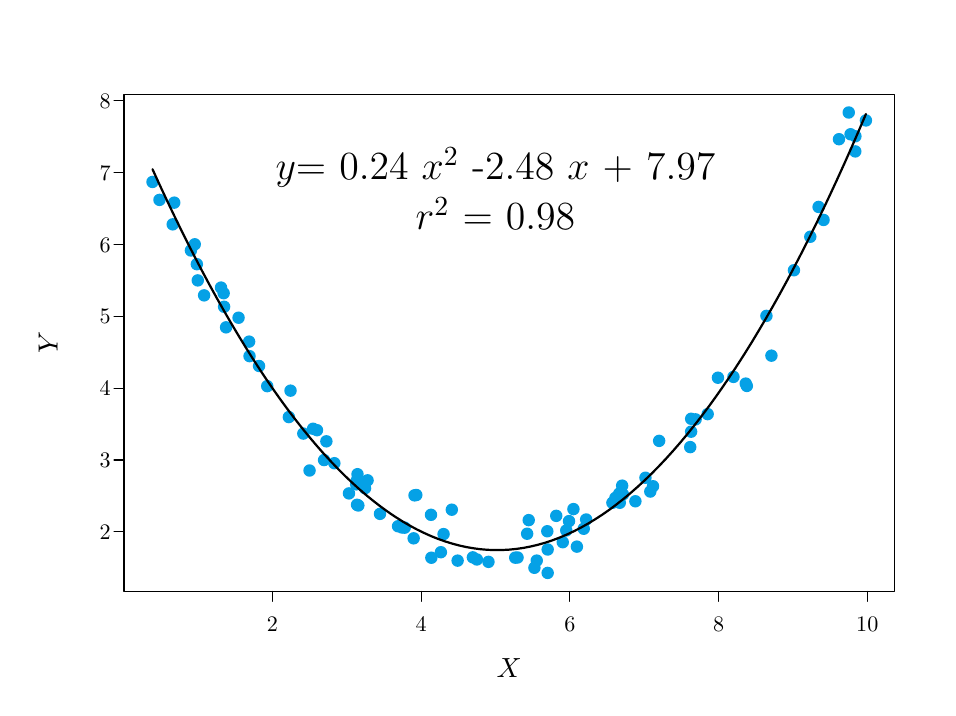
\begin{tikzpicture}[x=1pt,y=1pt]
\definecolor{fillColor}{RGB}{255,255,255}
\path[use as bounding box,fill=fillColor,fill opacity=0.00] (0,0) rectangle (325.21,238.49);
\begin{scope}
\path[clip] ( 34.80, 34.80) rectangle (313.21,214.49);
\definecolor{fillColor}{RGB}{5,161,230}

\path[fill=fillColor] ( 58.99,157.98) circle (  2.25);

\path[fill=fillColor] (139.47, 53.96) circle (  2.25);

\path[fill=fillColor] (297.34,199.97) circle (  2.25);

\path[fill=fillColor] (282.80,162.94) circle (  2.25);

\path[fill=fillColor] (119.48, 65.83) circle (  2.25);

\path[fill=fillColor] (287.59,169.01) circle (  2.25);

\path[fill=fillColor] (241.36, 96.94) circle (  2.25);

\path[fill=fillColor] (135.27, 57.88) circle (  2.25);

\path[fill=fillColor] (104.54, 93.04) circle (  2.25);

\path[fill=fillColor] (239.73, 92.50) circle (  2.25);

\path[fill=fillColor] (249.43,112.00) circle (  2.25);

\path[fill=fillColor] (195.62, 60.18) circle (  2.25);

\path[fill=fillColor] (119.18, 77.13) circle (  2.25);

\path[fill=fillColor] ( 83.60,116.24) circle (  2.25);

\path[fill=fillColor] (103.13, 93.56) circle (  2.25);

\path[fill=fillColor] (116.10, 70.20) circle (  2.25);

\path[fill=fillColor] (166.50, 45.46) circle (  2.25);

\path[fill=fillColor] (107.93, 89.02) circle (  2.25);

\path[fill=fillColor] (127.31, 62.80) circle (  2.25);

\path[fill=fillColor] (160.87, 47.09) circle (  2.25);

\path[fill=fillColor] ( 52.41,167.42) circle (  2.25);

\path[fill=fillColor] (201.81, 60.77) circle (  2.25);

\path[fill=fillColor] ( 61.13,153.03) circle (  2.25);

\path[fill=fillColor] (145.87, 46.96) circle (  2.25);

\path[fill=fillColor] (296.69,207.84) circle (  2.25);

\path[fill=fillColor] ( 52.95,175.26) circle (  2.25);

\path[fill=fillColor] (255.03,112.30) circle (  2.25);

\path[fill=fillColor] ( 69.87,144.57) circle (  2.25);

\path[fill=fillColor] ( 45.11,182.74) circle (  2.25);

\path[fill=fillColor] ( 70.81,142.54) circle (  2.25);

\path[fill=fillColor] (285.80,173.71) circle (  2.25);

\path[fill=fillColor] (239.41, 86.93) circle (  2.25);

\path[fill=fillColor] (213.96, 66.81) circle (  2.25);

\path[fill=fillColor] (122.82, 74.92) circle (  2.25);

\path[fill=fillColor] (187.90, 41.46) circle (  2.25);

\path[fill=fillColor] (118.71, 73.47) circle (  2.25);

\path[fill=fillColor] (183.95, 45.92) circle (  2.25);

\path[fill=fillColor] (194.62, 56.82) circle (  2.25);

\path[fill=fillColor] (153.26, 64.31) circle (  2.25);

\path[fill=fillColor] (119.02, 66.08) circle (  2.25);

\path[fill=fillColor] (145.74, 62.46) circle (  2.25);

\path[fill=fillColor] ( 70.98,137.64) circle (  2.25);

\path[fill=fillColor] (110.82, 81.11) circle (  2.25);

\path[fill=fillColor] (215.10, 69.84) circle (  2.25);

\path[fill=fillColor] (259.87,109.04) circle (  2.25);

\path[fill=fillColor] (191.00, 62.09) circle (  2.25);

\path[fill=fillColor] (155.36, 45.90) circle (  2.25);

\path[fill=fillColor] (214.81, 73.00) circle (  2.25);

\path[fill=fillColor] ( 63.75,141.76) circle (  2.25);

\path[fill=fillColor] (139.78, 69.49) circle (  2.25);

\path[fill=fillColor] (176.18, 46.98) circle (  2.25);

\path[fill=fillColor] (133.84, 58.33) circle (  2.25);

\path[fill=fillColor] (211.29, 66.80) circle (  2.25);

\path[fill=fillColor] (293.16,198.18) circle (  2.25);

\path[fill=fillColor] (177.01, 47.03) circle (  2.25);

\path[fill=fillColor] (181.05, 60.54) circle (  2.25);

\path[fill=fillColor] (150.28, 55.49) circle (  2.25);

\path[fill=fillColor] ( 61.47,147.17) circle (  2.25);

\path[fill=fillColor] (213.75, 70.13) circle (  2.25);

\path[fill=fillColor] ( 80.02,125.04) circle (  2.25);

\path[fill=fillColor] (193.35, 52.56) circle (  2.25);

\path[fill=fillColor] (187.90, 49.93) circle (  2.25);

\path[fill=fillColor] ( 71.69,130.20) circle (  2.25);

\path[fill=fillColor] (183.11, 43.32) circle (  2.25);

\path[fill=fillColor] ( 47.63,176.26) circle (  2.25);

\path[fill=fillColor] (200.93, 57.43) circle (  2.25);

\path[fill=fillColor] ( 94.98,107.32) circle (  2.25);

\path[fill=fillColor] (140.43, 69.62) circle (  2.25);

\path[fill=fillColor] (136.24, 57.82) circle (  2.25);

\path[fill=fillColor] ( 60.37,160.21) circle (  2.25);

\path[fill=fillColor] (225.96, 72.79) circle (  2.25);

\path[fill=fillColor] (266.95,134.35) circle (  2.25);

\path[fill=fillColor] ( 94.38, 97.78) circle (  2.25);

\path[fill=fillColor] ( 99.60, 91.82) circle (  2.25);

\path[fill=fillColor] (149.31, 48.94) circle (  2.25);

\path[fill=fillColor] ( 86.56,108.95) circle (  2.25);

\path[fill=fillColor] (107.10, 82.25) circle (  2.25);

\path[fill=fillColor] (101.86, 78.47) circle (  2.25);

\path[fill=fillColor] (224.98, 70.87) circle (  2.25);

\path[fill=fillColor] (121.91, 72.08) circle (  2.25);

\path[fill=fillColor] (212.38, 68.58) circle (  2.25);

\path[fill=fillColor] (239.75, 97.16) circle (  2.25);

\path[fill=fillColor] (228.18, 89.18) circle (  2.25);

\path[fill=fillColor] ( 80.17,119.79) circle (  2.25);

\path[fill=fillColor] (197.21, 64.53) circle (  2.25);

\path[fill=fillColor] (259.47,109.88) circle (  2.25);

\path[fill=fillColor] (245.71, 98.85) circle (  2.25);

\path[fill=fillColor] (162.32, 46.32) circle (  2.25);

\path[fill=fillColor] (302.90,204.96) circle (  2.25);

\path[fill=fillColor] (299.05,193.77) circle (  2.25);

\path[fill=fillColor] (276.89,150.83) circle (  2.25);

\path[fill=fillColor] (118.93, 74.87) circle (  2.25);

\path[fill=fillColor] (299.10,199.25) circle (  2.25);

\path[fill=fillColor] (198.46, 50.96) circle (  2.25);

\path[fill=fillColor] (180.48, 55.62) circle (  2.25);

\path[fill=fillColor] ( 76.20,133.68) circle (  2.25);

\path[fill=fillColor] (223.23, 75.85) circle (  2.25);

\path[fill=fillColor] (268.75,119.97) circle (  2.25);

\path[fill=fillColor] (219.60, 67.35) circle (  2.25);

\path[fill=fillColor] (187.77, 56.52) circle (  2.25);
\end{scope}
\begin{scope}
\path[clip] (  0.00,  0.00) rectangle (325.21,238.49);
\definecolor{drawColor}{RGB}{0,0,0}

\path[draw=drawColor,line width= 0.4pt,line join=round,line cap=round] ( 88.41, 34.80) -- (303.39, 34.80);

\path[draw=drawColor,line width= 0.4pt,line join=round,line cap=round] ( 88.41, 34.80) -- ( 88.41, 31.21);

\path[draw=drawColor,line width= 0.4pt,line join=round,line cap=round] (142.16, 34.80) -- (142.16, 31.21);

\path[draw=drawColor,line width= 0.4pt,line join=round,line cap=round] (195.90, 34.80) -- (195.90, 31.21);

\path[draw=drawColor,line width= 0.4pt,line join=round,line cap=round] (249.65, 34.80) -- (249.65, 31.21);

\path[draw=drawColor,line width= 0.4pt,line join=round,line cap=round] (303.39, 34.80) -- (303.39, 31.21);

\node[text=drawColor,anchor=base,inner sep=0pt, outer sep=0pt, scale=  0.80] at ( 88.41, 20.40) {2};

\node[text=drawColor,anchor=base,inner sep=0pt, outer sep=0pt, scale=  0.80] at (142.16, 20.40) {4};

\node[text=drawColor,anchor=base,inner sep=0pt, outer sep=0pt, scale=  0.80] at (195.90, 20.40) {6};

\node[text=drawColor,anchor=base,inner sep=0pt, outer sep=0pt, scale=  0.80] at (249.65, 20.40) {8};

\node[text=drawColor,anchor=base,inner sep=0pt, outer sep=0pt, scale=  0.80] at (303.39, 20.40) {10};

\path[draw=drawColor,line width= 0.4pt,line join=round,line cap=round] ( 34.80, 56.32) -- ( 34.80,212.09);

\path[draw=drawColor,line width= 0.4pt,line join=round,line cap=round] ( 34.80, 56.32) -- ( 31.21, 56.32);

\path[draw=drawColor,line width= 0.4pt,line join=round,line cap=round] ( 34.80, 82.28) -- ( 31.21, 82.28);

\path[draw=drawColor,line width= 0.4pt,line join=round,line cap=round] ( 34.80,108.25) -- ( 31.21,108.25);

\path[draw=drawColor,line width= 0.4pt,line join=round,line cap=round] ( 34.80,134.21) -- ( 31.21,134.21);

\path[draw=drawColor,line width= 0.4pt,line join=round,line cap=round] ( 34.80,160.17) -- ( 31.21,160.17);

\path[draw=drawColor,line width= 0.4pt,line join=round,line cap=round] ( 34.80,186.13) -- ( 31.21,186.13);

\path[draw=drawColor,line width= 0.4pt,line join=round,line cap=round] ( 34.80,212.09) -- ( 31.21,212.09);

\node[text=drawColor,anchor=base east,inner sep=0pt, outer sep=0pt, scale=  0.80] at ( 30.00, 53.57) {2};

\node[text=drawColor,anchor=base east,inner sep=0pt, outer sep=0pt, scale=  0.80] at ( 30.00, 79.53) {3};

\node[text=drawColor,anchor=base east,inner sep=0pt, outer sep=0pt, scale=  0.80] at ( 30.00,105.49) {4};

\node[text=drawColor,anchor=base east,inner sep=0pt, outer sep=0pt, scale=  0.80] at ( 30.00,131.45) {5};

\node[text=drawColor,anchor=base east,inner sep=0pt, outer sep=0pt, scale=  0.80] at ( 30.00,157.41) {6};

\node[text=drawColor,anchor=base east,inner sep=0pt, outer sep=0pt, scale=  0.80] at ( 30.00,183.37) {7};

\node[text=drawColor,anchor=base east,inner sep=0pt, outer sep=0pt, scale=  0.80] at ( 30.00,209.33) {8};

\path[draw=drawColor,line width= 0.4pt,line join=round,line cap=round] ( 34.80, 34.80) --
	(313.21, 34.80) --
	(313.21,214.49) --
	( 34.80,214.49) --
	( 34.80, 34.80);
\end{scope}
\begin{scope}
\path[clip] (  0.00,  0.00) rectangle (325.21,238.49);
\definecolor{drawColor}{RGB}{0,0,0}

\node[text=drawColor,anchor=base,inner sep=0pt, outer sep=0pt, scale=  1.00] at (174.01,  3.60) {$X$};

\node[text=drawColor,rotate= 90.00,anchor=base,inner sep=0pt, outer sep=0pt, scale=  1.00] at ( 10.80,124.65) {$Y$};
\end{scope}
\begin{scope}
\path[clip] ( 34.80, 34.80) rectangle (313.21,214.49);
\definecolor{drawColor}{RGB}{0,0,0}

\path[draw=drawColor,line width= 0.8pt,line join=round,line cap=round] ( 45.11,187.33) --
	( 47.69,181.69) --
	( 50.27,176.17) --
	( 52.85,170.77) --
	( 55.42,165.48) --
	( 58.00,160.31) --
	( 60.58,155.27) --
	( 63.16,150.33) --
	( 65.73,145.52) --
	( 68.31,140.83) --
	( 70.89,136.25) --
	( 73.47,131.79) --
	( 76.05,127.45) --
	( 78.62,123.23) --
	( 81.20,119.12) --
	( 83.78,115.13) --
	( 86.36,111.26) --
	( 88.94,107.51) --
	( 91.51,103.88) --
	( 94.09,100.36) --
	( 96.67, 96.97) --
	( 99.25, 93.69) --
	(101.83, 90.52) --
	(104.40, 87.48) --
	(106.98, 84.55) --
	(109.56, 81.75) --
	(112.14, 79.06) --
	(114.72, 76.48) --
	(117.29, 74.03) --
	(119.87, 71.69) --
	(122.45, 69.48) --
	(125.03, 67.38) --
	(127.61, 65.39) --
	(130.18, 63.53) --
	(132.76, 61.78) --
	(135.34, 60.15) --
	(137.92, 58.64) --
	(140.49, 57.25) --
	(143.07, 55.98) --
	(145.65, 54.82) --
	(148.23, 53.78) --
	(150.81, 52.86) --
	(153.38, 52.06) --
	(155.96, 51.37) --
	(158.54, 50.80) --
	(161.12, 50.36) --
	(163.70, 50.02) --
	(166.27, 49.81) --
	(168.85, 49.72) --
	(171.43, 49.74) --
	(174.01, 49.88) --
	(176.59, 50.14) --
	(179.16, 50.51) --
	(181.74, 51.01) --
	(184.32, 51.62) --
	(186.90, 52.35) --
	(189.47, 53.20) --
	(192.05, 54.17) --
	(194.63, 55.25) --
	(197.21, 56.45) --
	(199.79, 57.77) --
	(202.36, 59.21) --
	(204.94, 60.77) --
	(207.52, 62.44) --
	(210.10, 64.23) --
	(212.68, 66.14) --
	(215.25, 68.17) --
	(217.83, 70.32) --
	(220.41, 72.58) --
	(222.99, 74.96) --
	(225.57, 77.46) --
	(228.14, 80.08) --
	(230.72, 82.81) --
	(233.30, 85.67) --
	(235.88, 88.64) --
	(238.46, 91.73) --
	(241.03, 94.94) --
	(243.61, 98.26) --
	(246.19,101.70) --
	(248.77,105.27) --
	(251.34,108.94) --
	(253.92,112.74) --
	(256.50,116.66) --
	(259.08,120.69) --
	(261.66,124.84) --
	(264.23,129.11) --
	(266.81,133.50) --
	(269.39,138.00) --
	(271.97,142.62) --
	(274.55,147.36) --
	(277.12,152.22) --
	(279.70,157.20) --
	(282.28,162.29) --
	(284.86,167.51) --
	(287.44,172.84) --
	(290.01,178.28) --
	(292.59,183.85) --
	(295.17,189.53) --
	(297.75,195.34) --
	(300.33,201.26) --
	(302.90,207.29);

\node[text=drawColor,anchor=base,inner sep=0pt, outer sep=0pt, scale=  1.00] at (169.03,183.63) {\Large $y$= 0.24 $x^2$ -2.48 $x$ + 7.97};

\node[text=drawColor,anchor=base,inner sep=0pt, outer sep=0pt, scale=  1.00] at (169.03,165.45) {\Large $r^2$ = 0.98};
\end{scope}
\end{tikzpicture}
}
\end{center}
\end{frame}


%---------------------------------------------------------------------slide----
\begin{frame}
\frametitle{Outliers in regression}
Outliers in regression studies are points that clearly do not follow the tendency of the rest of points, even if the values of the pair are not outliers for every variable separately.
\begin{center}
\tikzsetnextfilename{regression/scatterplot_with_outliers}
\resizebox{0.7\textwidth}{!}{\input{img/regression/scatterplot_with_outliers}}
\end{center}
\end{frame}


%---------------------------------------------------------------------slide----
\begin{frame}
\frametitle{Outliers influence in regression}
Outliers in regression studies can provoke drastic changes in the regression models. 
\begin{center}
\tikzsetnextfilename{regression/linear_regression_with_outliers}
\resizebox{0.49\textwidth}{!}{% Created by tikzDevice version 0.9 on 2016-02-25 17:09:39
% !TEX encoding = UTF-8 Unicode
\begin{tikzpicture}[x=1pt,y=1pt]
\definecolor{fillColor}{RGB}{255,255,255}
\path[use as bounding box,fill=fillColor,fill opacity=0.00] (0,0) rectangle (505.89,361.35);
\begin{scope}
\path[clip] ( 72.27, 72.27) rectangle (469.75,325.21);
\definecolor{fillColor}{RGB}{5,161,230}

\path[fill=fillColor] (342.90,115.86) circle (  2.25);

\path[fill=fillColor] (127.43,179.71) circle (  2.25);

\path[fill=fillColor] (385.50,103.53) circle (  2.25);

\path[fill=fillColor] (189.81,164.06) circle (  2.25);

\path[fill=fillColor] ( 88.69,199.18) circle (  2.25);

\path[fill=fillColor] (304.50,125.99) circle (  2.25);

\path[fill=fillColor] (261.91,145.02) circle (  2.25);

\path[fill=fillColor] (347.05,110.24) circle (  2.25);

\path[fill=fillColor] (134.47,177.32) circle (  2.25);

\path[fill=fillColor] (381.43,269.00) circle (  2.25);
\end{scope}
\begin{scope}
\path[clip] (  0.00,  0.00) rectangle (505.89,361.35);
\definecolor{drawColor}{RGB}{0,0,0}

\path[draw=drawColor,line width= 0.4pt,line join=round,line cap=round] ( 86.99, 72.27) -- (455.03, 72.27);

\path[draw=drawColor,line width= 0.4pt,line join=round,line cap=round] ( 86.99, 72.27) -- ( 86.99, 66.27);

\path[draw=drawColor,line width= 0.4pt,line join=round,line cap=round] (160.60, 72.27) -- (160.60, 66.27);

\path[draw=drawColor,line width= 0.4pt,line join=round,line cap=round] (234.21, 72.27) -- (234.21, 66.27);

\path[draw=drawColor,line width= 0.4pt,line join=round,line cap=round] (307.82, 72.27) -- (307.82, 66.27);

\path[draw=drawColor,line width= 0.4pt,line join=round,line cap=round] (381.43, 72.27) -- (381.43, 66.27);

\path[draw=drawColor,line width= 0.4pt,line join=round,line cap=round] (455.03, 72.27) -- (455.03, 66.27);

\node[text=drawColor,anchor=base,inner sep=0pt, outer sep=0pt, scale=  1.00] at ( 86.99, 50.67) {0};

\node[text=drawColor,anchor=base,inner sep=0pt, outer sep=0pt, scale=  1.00] at (160.60, 50.67) {2};

\node[text=drawColor,anchor=base,inner sep=0pt, outer sep=0pt, scale=  1.00] at (234.21, 50.67) {4};

\node[text=drawColor,anchor=base,inner sep=0pt, outer sep=0pt, scale=  1.00] at (307.82, 50.67) {6};

\node[text=drawColor,anchor=base,inner sep=0pt, outer sep=0pt, scale=  1.00] at (381.43, 50.67) {8};

\node[text=drawColor,anchor=base,inner sep=0pt, outer sep=0pt, scale=  1.00] at (455.03, 50.67) {10};

\path[draw=drawColor,line width= 0.4pt,line join=round,line cap=round] ( 72.27, 81.64) -- ( 72.27,315.85);

\path[draw=drawColor,line width= 0.4pt,line join=round,line cap=round] ( 72.27, 81.64) -- ( 66.27, 81.64);

\path[draw=drawColor,line width= 0.4pt,line join=round,line cap=round] ( 72.27,128.48) -- ( 66.27,128.48);

\path[draw=drawColor,line width= 0.4pt,line join=round,line cap=round] ( 72.27,175.32) -- ( 66.27,175.32);

\path[draw=drawColor,line width= 0.4pt,line join=round,line cap=round] ( 72.27,222.16) -- ( 66.27,222.16);

\path[draw=drawColor,line width= 0.4pt,line join=round,line cap=round] ( 72.27,269.00) -- ( 66.27,269.00);

\path[draw=drawColor,line width= 0.4pt,line join=round,line cap=round] ( 72.27,315.85) -- ( 66.27,315.85);

\node[text=drawColor,rotate= 90.00,anchor=base,inner sep=0pt, outer sep=0pt, scale=  1.00] at ( 57.87, 81.64) {0};

\node[text=drawColor,rotate= 90.00,anchor=base,inner sep=0pt, outer sep=0pt, scale=  1.00] at ( 57.87,128.48) {2};

\node[text=drawColor,rotate= 90.00,anchor=base,inner sep=0pt, outer sep=0pt, scale=  1.00] at ( 57.87,175.32) {4};

\node[text=drawColor,rotate= 90.00,anchor=base,inner sep=0pt, outer sep=0pt, scale=  1.00] at ( 57.87,222.16) {6};

\node[text=drawColor,rotate= 90.00,anchor=base,inner sep=0pt, outer sep=0pt, scale=  1.00] at ( 57.87,269.00) {8};

\node[text=drawColor,rotate= 90.00,anchor=base,inner sep=0pt, outer sep=0pt, scale=  1.00] at ( 57.87,315.85) {10};

\path[draw=drawColor,line width= 0.4pt,line join=round,line cap=round] ( 72.27, 72.27) --
	(469.75, 72.27) --
	(469.75,325.21) --
	( 72.27,325.21) --
	( 72.27, 72.27);
\end{scope}
\begin{scope}
\path[clip] (  0.00,  0.00) rectangle (505.89,361.35);
\definecolor{drawColor}{RGB}{0,0,0}

\node[text=drawColor,anchor=base,inner sep=0pt, outer sep=0pt, scale=  1.20] at (271.01,339.14) {\bfseries Linear regression with outliers};

\node[text=drawColor,anchor=base,inner sep=0pt, outer sep=0pt, scale=  1.20] at (271.01, 26.67) {$X$};

\node[text=drawColor,rotate= 90.00,anchor=base,inner sep=0pt, outer sep=0pt, scale=  1.20] at ( 33.87,198.74) {$Y$};
\end{scope}
\begin{scope}
\path[clip] ( 72.27, 72.27) rectangle (469.75,325.21);
\definecolor{drawColor}{RGB}{0,0,0}

\path[draw=drawColor,line width= 0.8pt,line join=round,line cap=round] ( 72.27,183.46) -- (469.76,130.63);

\node[text=drawColor,anchor=base,inner sep=0pt, outer sep=0pt, scale=  1.00] at (271.01,243.08) {\Large $y$= -0.21 x + 4.26};

\node[text=drawColor,anchor=base,inner sep=0pt, outer sep=0pt, scale=  1.00] at (271.01,226.37) {\Large $r^2$ = 0.08};
\end{scope}
\end{tikzpicture}
}
\tikzsetnextfilename{regression/linear_regression_without_outliers}
\resizebox{0.49\textwidth}{!}{\input{img/regression/linear_regression_without_outliers}}
\end{center}
\end{frame}


%---------------------------------------------------------------------slide----
\begin{frame}
\frametitle{Simpson's paradox}
Sometimes a trend can disappears or even reverses when we split the sample into groups according to a qualitative variable that is related to the dependent variable.
This is known as the \emph{Simpson's paradox}. 
\begin{center}
\tikzsetnextfilename{regression/simpson_paradox_1}
\resizebox{0.7\textwidth}{!}{% Created by tikzDevice version 0.12.3 on 2019-09-02 17:55:25
% !TEX encoding = UTF-8 Unicode
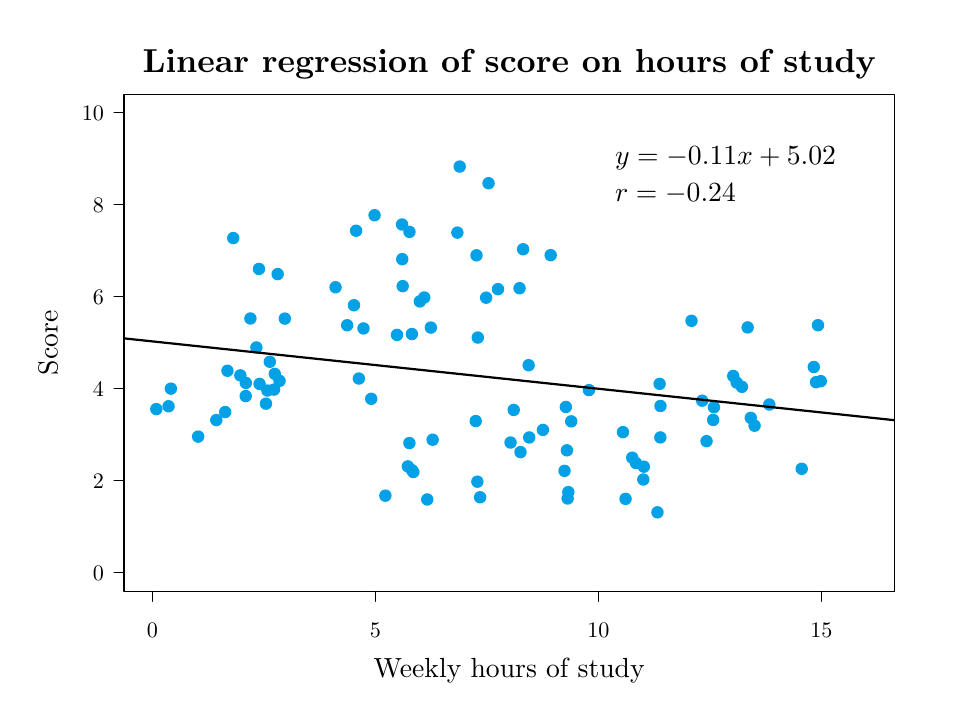
\begin{tikzpicture}[x=1pt,y=1pt]
\definecolor{fillColor}{RGB}{255,255,255}
\path[use as bounding box,fill=fillColor,fill opacity=0.00] (0,0) rectangle (325.21,238.49);
\begin{scope}
\path[clip] ( 34.80, 34.80) rectangle (313.21,214.49);
\definecolor{fillColor}{RGB}{5,161,230}

\path[fill=fillColor] ( 61.60, 90.72) circle (  2.25);

\path[fill=fillColor] (135.35,154.84) circle (  2.25);

\path[fill=fillColor] (133.46,127.47) circle (  2.25);

\path[fill=fillColor] (135.51,145.09) circle (  2.25);

\path[fill=fillColor] (169.95,144.00) circle (  2.25);

\path[fill=fillColor] (137.96,164.70) circle (  2.25);

\path[fill=fillColor] ( 46.49,100.66) circle (  2.25);

\path[fill=fillColor] ( 78.83,110.13) circle (  2.25);

\path[fill=fillColor] (141.70,139.56) circle (  2.25);

\path[fill=fillColor] (119.68,111.70) circle (  2.25);

\path[fill=fillColor] (145.69,130.12) circle (  2.25);

\path[fill=fillColor] (124.14,104.38) circle (  2.25);

\path[fill=fillColor] ( 86.11,102.63) circle (  2.25);

\path[fill=fillColor] (179.02,158.42) circle (  2.25);

\path[fill=fillColor] ( 87.50,117.76) circle (  2.25);

\path[fill=fillColor] (166.53,182.28) circle (  2.25);

\path[fill=fillColor] ( 86.62,107.37) circle (  2.25);

\path[fill=fillColor] ( 83.80,109.76) circle (  2.25);

\path[fill=fillColor] ( 72.19,114.52) circle (  2.25);

\path[fill=fillColor] ( 78.79,105.37) circle (  2.25);

\path[fill=fillColor] ( 91.02,110.86) circle (  2.25);

\path[fill=fillColor] ( 89.00,107.71) circle (  2.25);

\path[fill=fillColor] ( 68.17, 96.70) circle (  2.25);

\path[fill=fillColor] ( 50.91,101.69) circle (  2.25);

\path[fill=fillColor] ( 76.84,112.85) circle (  2.25);

\path[fill=fillColor] (162.65,126.51) circle (  2.25);

\path[fill=fillColor] (121.34,129.81) circle (  2.25);

\path[fill=fillColor] (177.74,144.34) circle (  2.25);

\path[fill=fillColor] (165.66,140.92) circle (  2.25);

\path[fill=fillColor] ( 51.75,108.05) circle (  2.25);

\path[fill=fillColor] (111.25,144.69) circle (  2.25);

\path[fill=fillColor] ( 83.57,151.31) circle (  2.25);

\path[fill=fillColor] ( 89.29,113.39) circle (  2.25);

\path[fill=fillColor] (118.68,165.11) circle (  2.25);

\path[fill=fillColor] ( 71.37, 99.59) circle (  2.25);

\path[fill=fillColor] (155.27,164.43) circle (  2.25);

\path[fill=fillColor] ( 74.29,162.47) circle (  2.25);

\path[fill=fillColor] ( 82.64,122.93) circle (  2.25);

\path[fill=fillColor] (188.98,156.29) circle (  2.25);

\path[fill=fillColor] (162.18,156.24) circle (  2.25);

\path[fill=fillColor] (125.35,170.72) circle (  2.25);

\path[fill=fillColor] (138.85,127.78) circle (  2.25);

\path[fill=fillColor] ( 90.33,149.44) circle (  2.25);

\path[fill=fillColor] (135.28,167.37) circle (  2.25);

\path[fill=fillColor] ( 92.93,133.36) circle (  2.25);

\path[fill=fillColor] (117.91,138.19) circle (  2.25);

\path[fill=fillColor] (143.30,140.99) circle (  2.25);

\path[fill=fillColor] (115.44,130.96) circle (  2.25);

\path[fill=fillColor] ( 80.48,133.40) circle (  2.25);

\path[fill=fillColor] (156.11,188.30) circle (  2.25);

\path[fill=fillColor] (196.41, 96.24) circle (  2.25);

\path[fill=fillColor] (162.50, 74.44) circle (  2.25);

\path[fill=fillColor] (138.91, 78.56) circle (  2.25);

\path[fill=fillColor] (262.67, 94.66) circle (  2.25);

\path[fill=fillColor] (163.48, 68.80) circle (  2.25);

\path[fill=fillColor] (284.88,110.39) circle (  2.25);

\path[fill=fillColor] (222.65, 79.85) circle (  2.25);

\path[fill=fillColor] (286.59,110.76) circle (  2.25);

\path[fill=fillColor] (186.19, 93.14) circle (  2.25);

\path[fill=fillColor] (215.11, 92.34) circle (  2.25);

\path[fill=fillColor] (194.86, 85.76) circle (  2.25);

\path[fill=fillColor] (218.46, 83.10) circle (  2.25);

\path[fill=fillColor] (195.36, 70.66) circle (  2.25);

\path[fill=fillColor] (161.90, 96.34) circle (  2.25);

\path[fill=fillColor] (139.36, 77.93) circle (  2.25);

\path[fill=fillColor] (228.35,109.77) circle (  2.25);

\path[fill=fillColor] (195.12, 68.37) circle (  2.25);

\path[fill=fillColor] (137.39, 79.96) circle (  2.25);

\path[fill=fillColor] (254.95,112.63) circle (  2.25);

\path[fill=fillColor] (178.08, 85.12) circle (  2.25);

\path[fill=fillColor] (247.69, 96.75) circle (  2.25);

\path[fill=fillColor] (219.81, 81.16) circle (  2.25);

\path[fill=fillColor] (239.88,132.56) circle (  2.25);

\path[fill=fillColor] (194.47,101.43) circle (  2.25);

\path[fill=fillColor] (181.03,116.52) circle (  2.25);

\path[fill=fillColor] (247.98,101.32) circle (  2.25);

\path[fill=fillColor] (193.99, 78.34) circle (  2.25);

\path[fill=fillColor] (216.04, 68.22) circle (  2.25);

\path[fill=fillColor] (144.38, 68.01) circle (  2.25);

\path[fill=fillColor] (174.49, 88.58) circle (  2.25);

\path[fill=fillColor] (202.82,107.53) circle (  2.25);

\path[fill=fillColor] (181.23, 90.41) circle (  2.25);

\path[fill=fillColor] (222.46, 75.22) circle (  2.25);

\path[fill=fillColor] (137.93, 88.39) circle (  2.25);

\path[fill=fillColor] (279.70, 79.09) circle (  2.25);

\path[fill=fillColor] (129.25, 69.38) circle (  2.25);

\path[fill=fillColor] (261.29, 97.48) circle (  2.25);

\path[fill=fillColor] (227.57, 63.36) circle (  2.25);

\path[fill=fillColor] (175.63,100.36) circle (  2.25);

\path[fill=fillColor] (245.31, 89.08) circle (  2.25);

\path[fill=fillColor] (228.61, 90.43) circle (  2.25);

\path[fill=fillColor] (285.59,130.97) circle (  2.25);

\path[fill=fillColor] (146.34, 89.59) circle (  2.25);

\path[fill=fillColor] (267.98,102.32) circle (  2.25);

\path[fill=fillColor] (256.19,110.24) circle (  2.25);

\path[fill=fillColor] (258.09,108.72) circle (  2.25);

\path[fill=fillColor] (260.16,130.17) circle (  2.25);

\path[fill=fillColor] (243.73,103.70) circle (  2.25);

\path[fill=fillColor] (284.06,115.87) circle (  2.25);

\path[fill=fillColor] (228.66,101.78) circle (  2.25);
\end{scope}
\begin{scope}
\path[clip] (  0.00,  0.00) rectangle (325.21,238.49);
\definecolor{drawColor}{RGB}{0,0,0}

\path[draw=drawColor,line width= 0.4pt,line join=round,line cap=round] ( 45.11, 34.80) -- (286.79, 34.80);

\path[draw=drawColor,line width= 0.4pt,line join=round,line cap=round] ( 45.11, 34.80) -- ( 45.11, 31.21);

\path[draw=drawColor,line width= 0.4pt,line join=round,line cap=round] (125.67, 34.80) -- (125.67, 31.21);

\path[draw=drawColor,line width= 0.4pt,line join=round,line cap=round] (206.23, 34.80) -- (206.23, 31.21);

\path[draw=drawColor,line width= 0.4pt,line join=round,line cap=round] (286.79, 34.80) -- (286.79, 31.21);

\node[text=drawColor,anchor=base,inner sep=0pt, outer sep=0pt, scale=  0.80] at ( 45.11, 18.00) {0};

\node[text=drawColor,anchor=base,inner sep=0pt, outer sep=0pt, scale=  0.80] at (125.67, 18.00) {5};

\node[text=drawColor,anchor=base,inner sep=0pt, outer sep=0pt, scale=  0.80] at (206.23, 18.00) {10};

\node[text=drawColor,anchor=base,inner sep=0pt, outer sep=0pt, scale=  0.80] at (286.79, 18.00) {15};

\path[draw=drawColor,line width= 0.4pt,line join=round,line cap=round] ( 34.80, 41.46) -- ( 34.80,207.84);

\path[draw=drawColor,line width= 0.4pt,line join=round,line cap=round] ( 34.80, 41.46) -- ( 31.21, 41.46);

\path[draw=drawColor,line width= 0.4pt,line join=round,line cap=round] ( 34.80, 74.73) -- ( 31.21, 74.73);

\path[draw=drawColor,line width= 0.4pt,line join=round,line cap=round] ( 34.80,108.01) -- ( 31.21,108.01);

\path[draw=drawColor,line width= 0.4pt,line join=round,line cap=round] ( 34.80,141.28) -- ( 31.21,141.28);

\path[draw=drawColor,line width= 0.4pt,line join=round,line cap=round] ( 34.80,174.56) -- ( 31.21,174.56);

\path[draw=drawColor,line width= 0.4pt,line join=round,line cap=round] ( 34.80,207.84) -- ( 31.21,207.84);

\node[text=drawColor,anchor=base east,inner sep=0pt, outer sep=0pt, scale=  0.80] at ( 27.60, 38.70) {0};

\node[text=drawColor,anchor=base east,inner sep=0pt, outer sep=0pt, scale=  0.80] at ( 27.60, 71.98) {2};

\node[text=drawColor,anchor=base east,inner sep=0pt, outer sep=0pt, scale=  0.80] at ( 27.60,105.25) {4};

\node[text=drawColor,anchor=base east,inner sep=0pt, outer sep=0pt, scale=  0.80] at ( 27.60,138.53) {6};

\node[text=drawColor,anchor=base east,inner sep=0pt, outer sep=0pt, scale=  0.80] at ( 27.60,171.80) {8};

\node[text=drawColor,anchor=base east,inner sep=0pt, outer sep=0pt, scale=  0.80] at ( 27.60,205.08) {10};

\path[draw=drawColor,line width= 0.4pt,line join=round,line cap=round] ( 34.80, 34.80) --
	(313.21, 34.80) --
	(313.21,214.49) --
	( 34.80,214.49) --
	( 34.80, 34.80);
\end{scope}
\begin{scope}
\path[clip] (  0.00,  0.00) rectangle (325.21,238.49);
\definecolor{drawColor}{RGB}{0,0,0}

\node[text=drawColor,anchor=base,inner sep=0pt, outer sep=0pt, scale=  1.20] at (174.01,222.30) {\bfseries Linear regression of score on hours of study};

\node[text=drawColor,anchor=base,inner sep=0pt, outer sep=0pt, scale=  1.00] at (174.01,  3.60) {Weekly hours of study};

\node[text=drawColor,rotate= 90.00,anchor=base,inner sep=0pt, outer sep=0pt, scale=  1.00] at ( 10.80,124.65) {Score};
\end{scope}
\begin{scope}
\path[clip] ( 34.80, 34.80) rectangle (313.21,214.49);
\definecolor{drawColor}{RGB}{0,0,0}

\path[draw=drawColor,line width= 0.8pt,line join=round,line cap=round] ( 34.80,126.22) -- (313.21, 96.65);

\node[text=drawColor,anchor=base west,inner sep=0pt, outer sep=0pt, scale=  1.00] at (212.23,188.90) {$y= -0.11 x + 5.02 $};

\node[text=drawColor,anchor=base west,inner sep=0pt, outer sep=0pt, scale=  1.00] at (212.23,175.59) {$r= -0.24 $};
\end{scope}
\end{tikzpicture}
}
\end{center}
\end{frame}


%---------------------------------------------------------------------slide----

\begin{frame}
\frametitle{Simpson's paradox}
Sometimes a trend can disappears or even reverses when we split the sample into groups according to a qualitative variable that is related to the dependent variable.
This is known as the \emph{Simpson's paradox}. 
\begin{center}
\tikzsetnextfilename{regression/simpson_paradox_2}
\resizebox{0.7\textwidth}{!}{\input{img/regression/simpson_paradox_2}}
\end{center}
\end{frame}


% \subsection{Medidas de relación entre atributos}
% %---------------------------------------------------------------------slide----
% \begin{frame}
% \frametitle{Relaciones entre atributos}
% Los modelos de regresión vistos sólo pueden aplicarse cuando las variables estudiadas son cuantitativas.
% 
% Cuando se desea estudiar la relación entre atributos, tanto ordinales como nominales, es necesario recurrir a otro tipo
% de medidas de relación o de asociación. En este tema veremos tres de ellas:
% \begin{itemize}
% \item Coeficiente de correlación de Spearman.
% \item Coeficiente chi-cuadrado.
% \item Coeficiente de contingencia.
% \end{itemize}
% 
% \note{La regresión sólo tiene sentido cuando cuando las variables estudiadas son cuantitativas.
% 
% Cuando se desea estudiar la relación entre atributos, tanto ordinales como nominales, es necesario recurrir a otro tipo
% de medidas de relación o de asociación. Veremos tres de las más importantes que son
% \begin{itemize}
% \item Coeficiente de correlación de Spearman.
% \item Coeficiente chi-cuadrado.
% \item Coeficiente de contingencia.
% \end{itemize}
% }
% \end{frame}
% 
% 
% %---------------------------------------------------------------------slide----
% \begin{frame}
% \frametitle{Coeficiente de correlación de Spearman}
% Cuando se tengan atributos ordinales es posible ordenar sus categorías y asignarles valores ordinales, de manera que se
% puede calcular el coeficiente de correlación lineal entre estos valores ordinales. 
% 
% Esta medida de relación entre el orden que ocupan las categorías de dos atributos ordinales se conoce como coeficiente
% ce correlación de Spearman, y puede demostrarse fácilmente que puede calcularse a partir de la siguiente fórmula
% 
% \begin{definicion}[Coeficiente de correlación de Spearman]
% Dada una muestra de $n$ individuos en los que se han medido dos atributos ordinales $X$ e $Y$, el coeficiente de
% correlación de Spearman se define como: 
% \[
% r_s = 1-\frac{6\sum d_i^2}{n(n^2-1)}
% \]
% donde $d_i$ es la diferencia entre el valor ordinal de $X$ y el valor ordinal de $Y$ del individuo $i$.
% \end{definicion}
% 
% \note{Si queremos estudiar la relación entre dos atributos ordinales, como sus categorías pueden ordenarse, una posibilidad tomar sus
% valores de orden, que serían numéricos, y calcular el coeficiente de correlación lineal entre los órdenes.
% 
% Esta medida se conoce como coeficiente de correlación de Spearman, que se representa como $r_s$ y también puede calcularse haciendo la suma
% de los cuadrados de las diferencias entre los números de orden del valor de $X$ e $Y$ en cada indiviudo, multiplicada por 6, dividida por el
% tamaño de la muestra multiplicado por el cuadrado del tamaño de la muestra menos 1 y restando el resultado del cociente a 1.
% }
% \end{frame}
% 
% 
% %---------------------------------------------------------------------slide----
% \begin{frame}
% \frametitle{Interpretación del coeficiente de correlación de Spearman}
% Como el coeficiente de correlación de Spearman es en el fondo el coeficiente de correlación lineal aplicado a los
% órdenes, se tiene:
% \[
% -1\leq r_s\leq 1,
% \]
% de manera que:
% \begin{itemize}
% \item Si $r_s=0$ entonces no existe relación entre los atributos ordinales.
% \item Si $r_s=1$ entonces los órdenes de los atributos coinciden y existe una relación directa perfercta.
% \item Si $r_s=-1$ entonces los órdenes de los atributos están invertidos y existe una relación inversa perfecta.
% \end{itemize}
% En general, cuanto más cerca de $1$ o $-1$ esté $r_s$, mayor será la relación entre los atributos, y cuanto más cerca
% de $0$, menor será la relación.
% 
% \note{Como el coeficiente de correlación de Spearman es en el fondo el coeficiente de correlación lineal aplicado a los
% órdenes, su valor estará entre -1 y 1 y se interpreta de manera similar al coeficiente de correlación lineal, es decir,
% \begin{itemize}
% \item Si $r_s=0$ entonces no existe relación entre los atributos ordinales.
% \item Si $r_s=1$ entonces los órdenes de los atributos coinciden y existe una relación directa perfercta.
% \item Si $r_s=-1$ entonces los órdenes de los atributos están invertidos y existe una relación inversa perfecta.
% \end{itemize}
% }
% \end{frame}
% 
% 
% %---------------------------------------------------------------------slide----
% \begin{frame}
% \frametitle{Cálculo del coeficiente de correlación de Spearman}
% \framesubtitle{Ejemplo}
% Una muestra de 5 alumnos realizaron dos tareas diferentes $X$ e $Y$, y se ordenaron de acuerdo a la destreza que
% manifestaron en cada tarea:
% \[
% \begin{array}{lrrrr}
% \hline
% \text{Alumnos} & X & Y & d_i & d_i^2\\
% \hline
% \text{Alumno 1} & 2 & 3 & -1 & 1\\
% \text{Alumno 2} & 5 & 4 & 1 & 1 \\
% \text{Alumno 3} & 1 & 2 & -1 & 1\\
% \text{Alumno 4} & 3 & 1 & 2 & 4\\
% \text{Alumno 5} & 4 & 5 & -1 & 1\\
% \hline
% \sum &  &  & 0 & 8 \\
% \hline
% \end{array}
% \]
% El coeficiente de correlación de Spearman para esta muestra es 
% \[
% r_s = 1-\frac{6\sum d_i^2}{n(n^2-1)} = 1- \frac{6\cdot 8}{5(5^2-1)} = 0.6,
% \]
% lo que indica que existe bastante relación directa entre las destrezas manifestadas en ambas tareas.
% 
% \note{Para ilustrar el cálculo del coeficiente de correlación de Spearman, supongamos una muestra de 5 alumnos que realizaron dos tareas
% diferentes $X$ e $Y$, y se ordenaron de acuerdo a la destreza que manifestaron en cada tarea.
% 
% El primer alumno fue el segundo con más destreza en la tarea $X$ y el tercero en la tarea $Y$ de manera que la diferencia entre los órdenes
% en $X$ e $Y$ es $-1$ y su cuadrado vale 1. El segundo alumno fue el peor en la tarea $X$ y el penúltimo en la tarea $Y$ de manera que la
% diferencia entre sus órdenes en $X$ e $Y$ vale también $-1$ y su cuadrado 1, etc.  
% 
% Una vez calculados los cuadrados de las diferencias entre los órdenes, se suman, se multiplican por 6 y se dividen por el cuadrado del
% tamaño de la muestra, que vale 5,  por el cuadrado del tamaño de la muestra menos, que es $5^2-1$ y finalmente el resultado del cociente se
% resta a 1. Esto nos da un coeficiente de correlación de Spearman de 0.6, lo cual indica que existe bastante relación directa entre las
% destrezas manifestadas en ambas tareas.
% }
% \end{frame}
% 
% 
% %---------------------------------------------------------------------slide----
% \begin{frame}
% \frametitle{Cálculo del coeficiente de correlación de Spearman}
% \framesubtitle{Ejemplo con empates}
% Cuando hay empates en el orden de las categorías se atribuye a cada valor empatado la media aritmética de los valores
% ordinales que hubieran ocupado esos individuos en caso de no haber estado empatados.
% 
% Si en el ejemplo anterior los alumnos 4 y 5 se hubiesen comportado igual en la primera tarea y los alumnos 3 y 4 se
% hubiesen comportado igual en la segunda tarea, entonces se tendría
% \[
% \begin{array}{lrrrr}
% \hline
% \text{Alumnos} & X & Y & d_i & d_i^2\\
% \hline
% \text{Alumno 1} & 2 & 3 & -1 & 1\\
% \text{Alumno 2} & 5 & 4 & 1 & 1 \\
% \text{Alumno 3} & 1 & 1.5 & -0.5 & 0.25\\
% \text{Alumno 4} & 3.5 & 1.5 & 2 & 4\\
% \text{Alumno 5} & 3.5 & 5 & -1.5 & 2.25\\
% \hline
% \sum &  &  & 0 & 8.5 \\
% \hline
% \end{array}
% \]
% El coeficiente de correlación de Spearman para esta muestra es 
% \[
% r_s = 1-\frac{6\sum d_i^2}{n(n^2-1)} = 1- \frac{6\cdot 8.5}{5(5^2-1)} = 0.58.
% \]
% 
% \note{Cuando haya individuos con la misma categoría del atributo, entonces dichos individuos recibirán el mismo número de orden y de manera
% que habrá empates en el orden. En tal caso se atribuye a cada valor empatado la media aritmética de los valores ordinales que hubieran
% ocupado esos individuos en caso de no haber estado empatados.
% 
% Si en ejemplo anterior los alumnos 4 y 5 se hubiesen comportado igual en la primera tarea, entonces como ambos ocupan la posición 3 y 4
% en la ordenación, se toma la media $3.5$ y se le asigna dicho valor a ambos. Del mismo modo, si los alumnos 3 y 4 se hubiesen comportado
% igual en la segunda tarea, como el orden que ocupan es el primero y el segundo, entonces a ambos se le asigna la media $1.5$.
% 
% El resto de los cálculos para el coeficiente de Spearman se haría igual que en el caso en que no había empates.
% }
% \end{frame}
% 
% 
% %---------------------------------------------------------------------slide----
% \begin{frame}
% \frametitle{Relación entre atributos nominales}
% Cuando se quiere estudiar la relación entre atributos nominales no tiene sentido calcular el coeficiente de correlación
% de Spearman ya que las categorías no pueden ordenarse.
% 
% Para estudiar la relación entre atributos nominales se utilizan medidas basadas en las frecuencias de la tabla de
% frecuencias bidimensional, que para atributos se suele llamar \emph{tabla de contingencia}.
% 
% \highlight{Ejemplo}} En un estudio para ver si existe relación entre el sexo y el hábito de fumar se ha tomado
% una muestra de 100 personas.
% La tabla de contingencia resultante es
% \[
% \begin{array}{|l|rr|r|} 
% \hline
% \text{Sexo}\backslash\text{Fuma} & \text{Si} & \text{No} & n_i\\
% \hline
% \text{Mujer} & 12 & 28 & 40 \\
% \text{Hombre} & 26 & 34 & 60 \\
% \hline
% n_j & 38 & 62 & 100\\
% \hline
% \end{array}
% \]
% Si el hábito de fumar fuese independiente del sexo, la proporción de fumadores en mujeres y hombres sería la misma.
% 
% \note{Cuando se quiere estudiar la relación entre atributos nominales no tiene sentido calcular el coeficiente de correlación
% de Spearman ya que las categorías no pueden ordenarse. En este caso se utilizan medidas basadas en las frecuencias de la tabla de
% frecuencias bidimensional, que para atributos se suele llamar \emph{tabla de contingencia}.
% 
% En este ejemplo tenemos una tabla de contingencia para los atributos sexo y hábito de fumar, ambos nominales. En la muestra hay 12 mujeres
% fumadoras, 28 no fumadoras, 26 hombres fumadores y 34 no fumadores. En total tenemos una muestra de tamaño 100. 
% 
% La forma de estudiar la relación entre el sexo y el hábito de fumar es por medio de las frecuencias relativas de cada par de categorías.
% Así, si el hábito de fumar fuese independiente del sexo, la proporción de fumadores en mujeres y hombres sería la misma, mientras que si
% hubiese dependencia, serían significativamente diferentes.
% }
% \end{frame}
% 
% 
% %---------------------------------------------------------------------slide----
% \begin{frame}
% \frametitle{Frecuencias teóricas o esperadas}
% En general, dada una tabla de contingencia para dos atributos $X$ e $Y$, 
% \[
% \begin{array}{|c|ccccc|c|}
% \hline
% X\backslash Y & y_1 & \cdots & y_j & \cdots & y_q & n_x\\
% \hline
% x_1 & n_{11} & \cdots & n_{1j} & \cdots & n_{1q} & n_{x_1}\\
% \vdots & \vdots & \ddots & \vdots & \ddots & \vdots & \vdots \\
% x_i & n_{i1} & \cdots & n_{ij} & \cdots & n_{iq} & n_{x_i}\\
% \vdots & \vdots & \ddots & \vdots & \ddots & \vdots & \vdots\\
% x_p & n_{p1} & \cdots & n_{pj} & \cdots & n_{pq} & n_{x_p} \\
% \hline
% n_y & n_{y_1} & \cdots & n_{y_j} & \cdots & n_{y_q} & n\\
% \hline
% \end{array}
% \]
% si $X$ e $Y$ fuesen independientes, para cualquier valor $y_j$ se tendría
% \[
% \frac{n_{1j}}{n_{x_1}} = \frac{n_{2j}}{n_{x_2}} = \cdots = \frac{n_{pj}}{n_{x_p}} = \frac{n_{1j}+\cdots
% +n_{pj}}{n_{x_1}+\cdots+n_{x_p}} = \frac{n_{y_j}}{n},
% \]
% de donde se deduce que
% \[
% n_{ij} = \frac{n_{x_i}n_{y_j}}{n}.
% \]
% 
% A esta última expresión se le llama \emph{frecuencia teórica} o \emph{frecuencia esperada} del par $(x_i,y_j)$. 
% 
% \note{En general, dada una tabla de contingencia pra dos atributos $X$ e $Y$, si las variables fuesen independientes, entonces la proporción
% de individuos que presentan el valor $y_j$ en la variable $Y$ entre los que presentan el valor $x_1$ en la variable $X$ sería la frecuencia
% absoluta del par $(x_i,y_j)$ $n_{ij}$ divida entre la frecuencia absoluta de $x_1$ y esta frecuencia sería la misma que la proporción de
% individuos con el valor $y_j$ en $Y$ entre los que presentan el valor $x_2$ en $X$, y en general, al ser independiente de $X$ sería la misma
% para cualquier otra categoría de $X$, de manera que todas serían iguales a la proporción total de individuos en la muestra con valor $y_j$
% en la variable $Y$, que se obtendría dividiendo la frecuencia absoluta de $y_j$ entre el tamaño de la muestra.
% 
% De esta igualdad se puede deducir que la frecuencia absoluta de cualquier par $(x_i,y_j)$ se podría calcular multiplicando las frecuencias
% absolutas de $x_i$, $n_i$ y $y_j$ que es $n_j$ y dividendo por el tamaño de la muestra.
% 
% A estas frecuencias calculadas bajo la hipótesis de independencia, se les llama \emph{frecuencia teóricas} o \emph{frecuencia esperadas}.
% }
% \end{frame}
% 
% 
% %---------------------------------------------------------------------slide----
% \begin{frame}
% \frametitle{Coeficiente chi-cuadrado $\chi^2$}
% Es posible estudiar la relación entre dos atributos $X$ e $Y$ comparando las frecuencias reales con las esperadas:
% \begin{definicion}[Coeficiente chi-cuadrado $\chi^2$]
% Dada una muestra de tamaño $n$ en la que se han medido dos atributos $X$ e $Y$, se define el coeficiente $\chi^2$ como
% \[
% \chi^2 = \sum_{i=1}^p\sum_{j=1}^q \frac{\left(n_{ij}-\frac{n_{x_i}n_{y_j}}{n}\right)^2}{\frac{n_{x_i}n_{y_j}}{n}},
% \]
% donde $p$ es el número de categorías de $X$ y $q$ el número de categorías de $Y$.
% \end{definicion}
% 
% Por ser suma de cuadrados, se cumple que 
% \[
% \chi^2 \geq 0,
% \]
% de manera que $\chi^2=0$ cuando los atributos son independientes, y crece a medida que aumenta la dependencia entre las variables.
% 
% \note{Una posible forma de estudiar la relación entre dos atributos nominales es comparar sus frecuencias absolutas reales con las esperadas
% bajo la hipótesis de indepencia. Esto es precisamente lo que hace un estadístico conocido como coeficiente chi-cuadrado, que se denota con
% la letra griega $\chi^2$ y se calcula sumando para cada par de la variable bidimensional los cuadrados de las diferencias entre las
% frecuencias reales y las frecuencias esperadas, dividos por las propias frecuencias esperadas.
% 
% Como se trata de una suma de cuadrados, el coeficiente chi-cuadrado siempre es positivo. Cuando los atributos sean independientes, las
% frecuencias reales coincidirán con las esperadas y todos los sumandos se anularán, de manera que el coeficiente chi-cuadrado valdrá cero. Y
% en la medida que cada vez haya más dependencia, las diferencias entre las frecuencias reales y las esperadas serán cada vez mayores de forma
% que el coeficiente chi-cuadrado será también mayor.
% }
% \end{frame}
% 
% 
% %---------------------------------------------------------------------slide----
% \begin{frame}
% \frametitle{Cálculo del coeficiente chi-cuadrado $\chi^2$}
% \framesubtitle{Ejemplo}
% Siguiendo con el ejemplo anterior, a partir de la tabla de contingencia 
% \[
% \begin{array}{|l|rr|r|} 
% \hline
% \text{Sexo}\backslash\text{Fuma} & \text{Si} & \text{No} & n_i\\
% \hline
% \text{Mujer} & 12 & 28 & 40 \\
% \text{Hombre} & 26 & 34 & 60 \\
% \hline
% n_j & 38 & 62 & 100\\
% \hline
% \end{array}
% \]
% se obtienen las siguientes frecuencias esperadas:
% \[
% \renewcommand{\arraystretch}{1.5}
% \begin{array}{|l|rr|r|} 
% \hline
% \text{Sexo\Fuma} & \text{Si} & \text{No} & n_i\\
% \hline
% \text{Mujer} & \frac{40\cdot 38}{100}=15.2 & \frac{40\cdot 62}{100}=24.8 & 40 \\
% \text{Hombre} & \frac{60\cdot 38}{100}=22.8 & \frac{60\cdot 62}{100}=37.2 & 60 \\
% \hline
% n_j & 38 & 62 & 100\\
% \hline
% \end{array}
% \]
% y el coeficiente $\chi^2$ vale
% \[
% \chi^2 = \frac{(12-15.2)^2}{15.2}+\frac{(28-24.8)^2}{24.8}+\frac{(26-22.8)^2}{22.8}+\frac{(34-37.2)^2}{37.2} = 1.81,
% \]
% lo que indica que no existe gran relación entre el sexo y el hábito de fumar.
% 
% \note{Siguiendo con el ejemplo del sexo y el hábito de fumar, a partir de la tabla de contingencia se calculan las frecuencias esperadas de
% cada par. La frecuencia esperada de mujeres fumadoras es el número de mujeres 40, por el número de personas fumadoras 38, dividido por el
% tamaño de la muestra 100, lo que da $15.2$. Etc. 
% 
% Una vez calculadas las frecuencias esperadas, para calcular el coeficiente chi-cuadrado vamos calculando los cuadrados de las diferencias
% entre las frecuencias reales y las esperadas, es decir, para las mujeres fumadoras sería $(12-15.2)^2$ y esto se divide por la frecuencia
% esperada $15.2$. Del mismo modo se calculan los sumandos para el resto de los pares y se realiza la suma, lo que nos da un coeficiente
% chi-cuadrado de $1.81$, que al ser un valor próximo a 0 indica que no hay gran relación entre el sexo y el hábito de fumar.
% }
% \end{frame}
% 
% 
% %---------------------------------------------------------------------slide----
% \begin{frame}
% \frametitle{Coeficiente de contingencia}
% El coeficiente $\chi^2$ depende del tamaño muestral, ya que al multiplicar por una constante las frecuencias de todas
% las casillas, su valor queda multiplicado por dicha constante, lo que podría llevarnos al equívoco de pensar que ha
% aumentado la relación, incluso cuando las proporciones se mantienen.
% En consecuencia el valor de $\chi^2$ no está acotado superiormente y resulta difícil de interpretar.
% 
% Para evitar estos problemas se suele utilizar el siguiente estadístico:
% \begin{definicion}[Coeficiente de contingencia]
% Dada una muestra de tamaño $n$ en la que se han medido dos atributos $X$ e $Y$, se define el \emph{coeficiente de
% contingencia} como 
% \[
% C = \sqrt{\frac{\chi^2}{\chi^2+n}}
% \]
% \end{definicion}
% 
% \note{El principal problema del coeficiente chi-cuadrado es que depende del tamaño muestral ya que se calcula a partir de las frecuencias
% absolutas, no de las relativas. De hecho, se puede comprobar que al multiplicar por una constante las frecuencias de todas
% las casillas de la tabla de contingencia, su valor queda multiplicado por dicha constante, lo que podría llevarnos al equívoco de pensar que
% ha aumentado la relación, incluso cuando las proporciones se mantienen. En consecuencia el valor de $\chi^2$ no está acotado superiormente y
% resulta difícil de interpretar.
% 
% Para evitar estos problemas suele utilizarse otro estadístico conocido como coeficiente de contingencia, que se denota $C$, y se calcula a
% partir del coeficiente chi-cuadrado haciendo la raíz del cociente entre el coeficiente-chi cuadrado entre el mismo coeficiente chi-cuadrado
% mas el tamaño de la muestra.
% }
% \end{frame}
% 
% 
% %---------------------------------------------------------------------slide----
% \begin{frame}
% \frametitle{Interpretación del coeficiente de contingencia}
% De la definición anterior se deduce que 
% \[
% 0\leq C\leq 1,
% \]
% de manera que cuando $C=0$ las variables son independientes, y crece a medida que aumenta la relación.
% 
% Aunque $C$ nunca puede llegar a valer 1, se puede demostrar que para tablas de contingencia con $k$ filas y $k$
% columnas, el valor máximo que puede alcanzar $C$ es $\sqrt{(k-1)/k}$.
% 
% \highlight{Ejemplo}} En el ejemplo anterior el coeficiente de contingencia vale
% \[
% C = \sqrt{\frac{1.81}{1.81+100}} = 0.13.
% \]
% Como se trata de una tabla de contingencia de $2\times 2$, el valor máximo que podría tomar el coeficiente de
% contingencia es $\sqrt{(2-1)/2}=\sqrt{1/2}=0.707$, y como $0.13$ está bastante lejos de este valor, se puede concluir
% que no existe demasiada relación entre el hábito de fumar y el sexo.
% 
% \note{De la definición del coeficiente de contingencia es fácil ver que, al ser el numerador siempre menor que el denominador, siempre
% estará entre 0 y 1, de manera que el coeficiente de contingencia será nulo cuando las variables sean independientes, y estará más próximo a
% 1 a medida que aumente la dependencia.
% 
% Aunque el coeficiente de contingencia nunca puede llegar a valer 1, se puede demostrar que para tablas de contingencia con $k$ filas y $k$
% columnas, el valor máximo que puede alcanzar es $\sqrt{(k-1)/k}$, de modo que se puede comparar con este valor.
% 
% En el ejemplo del sexo y el hábito de fumar, como el coeficiente chi-cuadrado valía $1.81$, el coeficiente de contingencia vale la
% raíz cuadrada de $1.81$ dividido entre $1.81$ más el tamaño de la muestra 100, lo que da $0.13$. Y como se trata de una tabla de
% contingencia de $2\times 2$, el valor máximo que podría tomar el coeficiente de contingencia es $\sqrt{(2-1)/2}=\sqrt{1/2}=0.707$, y como
% $0.13$ está bastante lejos de este valor, se puede concluir que no existe demasiada relación entre el hábito de fumar y el sexo.
% }
% \end{frame}
